% !TeX spellcheck = de_DE

\chapter{Studie}
\label{chap:study}

Nachdem die vorherigen Kapiteln den Ablauf des Projekts, den zu erstellenden Prototypen und die dabei verwendeten Methoden beschrieben haben, dient dieses Kapitel nun der Evaluierung des Prototypen.

\section{Einführung}
In der Analyse, während den Gesprächen mit der Feuerwehr, wurde deutlich, dass das Wärmebild allein für ein fehlendes \bzw fehlerhaftes räumliches Verständnis sorgt.
Zusätzlich spiegeln eine Materialien, wie Glas oder Metall, die Wärmestrahlung.
Feine Unterschiede und Objektübergänge sind in der Nähe von warmen \bzw heißen Gegenständen kaum auszumachen.
Auch existieren \enquote{fehlerhafte Wärmeflecke} an Stellen, an welchen für eine längere Zeitperiode warme Gegenstände waren, welche zum aktuellen Zeitpunkt aber nicht mehr da sind.
Zudem ist die Navigation mit Hilfe einer Wärmebildkamera in Räumen ohne merkbaren Temperaturunterschied schwierig, da sich die dargestellten Farben kaum unterscheiden.
Objekte gehen damit ineinander über.

Um nun zu evaluieren, ob der erstellte Prototyp mit der Einbindung einer Tiefenbildkamera für eine Verbesserung dieser Problematiken sorgt, wurden zwei Studien durchgeführt.
Die erste Studie wurde mit 16 jungen Erwachsenen durchgeführt, welche größtenteils einen Hintergrund in der Informatik, und weder Erfahrung mit Wärme- noch Tiefenbildkameras hatten.
Die zweite Studie erfolgte mit 11 Mitgliedern einer Feuerwehr, welche bis dato nur Erfahrungen mit einer Wärmebildkamera hatten.
Um den Prototypen qualitativ bewerten zu können, wurden die Probanden in beiden Studien vor diverse Aufgaben in einem abgedunkelten Raum gestellt.
Zu den Aufgaben zählten das Lokalisieren eines bestimmten warmen Gegenstands und das Schätzen von Entfernungen.
Zusätzlich wurde das Navigationsverhalten und die Interaktion mit diversen Hindernissen beobachtet.
Außerdem wurde die Nutzungsdauer der verschiedenen Modi gemessen und Interviews mit den Probanden durchgeführt.

Dabei stellte sich heraus, dass der Großteil der Probanden einen der Modi, welcher Tiefenbildinformationen erhält, bevorzugt zum navigieren benutzt und die Wärmebildfunktion hauptsächlich zur Lokalisierung des warmen Objekts verwendet wurde.
Die Bewertung des Prototypen fiel in den Interviews überwiegend positiv aus.

\section{Studie 1}
Diese Studie wurde zu einem frühen Zeitpunkt im Projekt durchgeführt, weshalb sie zum Einen als Möglichkeit der Problemidentifikation des Prototypen und andererseits als Bildmodi-Test genutzt wurde.
\Dh dass die Nutzungsdauer beider Modi besonders interessant ist, um zu testen, welche Kamera hauptsächlich zum Navigieren genutzt wird.

\subsection{Methode}
Die Probanden wurden in einen komplett abgedunkelten Keller geführt und mussten zuerst die Länge und Breite eines Nebenraums abschätzen.
Darauf wurden sie in einen anderen Raum geführt, in welchem ein Labyrinth mit diversen Hindernissen aufgebaut war.
Hier mussten sie eine Wärmflasche finden und zurück zum Eingang bringen.
Der unterstützende Prototyp, den die Probanden erhielten, bestand aus lediglich einer tragbaren Form einer Wärme- und Tiefenbildkamera, mit angebrachtem Handy als Anzeigemöglichkeit.
Nutzer hatten nur Wärme- oder Tiefenbild zur Verfügung.

\subsection{Design}
Jeder Proband wurde nur einmal in den Keller geführt und hatte diesen noch nie zuvor betreten.
Dazu gab es keine Einschränkung in der Auswahl, welchen Bildmodus die Probanden nutzen dürfen.
Auch ihre Bewegungen wurden nicht eingeschränkt oder in eine Richtung geleitet.

\subsubsection{Probanden}
Zur Studiendurchführung wurden 16 Probanden zwischen 20 und 30 Jahren befragt.
Aus dieser Gruppe hat noch niemand bisherige Erfahrungen mit Wärmebild- oder Tiefenbildkameras gesammelt.
Die Probanden kamen dabei aus unterschiedlichen Berufsfeldern, wobei ein Großteil einen Hintergrund in der Informatik hatte.
25\% der Probanden waren weiblich.

\subsection{Vorgehen}

\subsubsection{Die Aufgabe}
Die Probanden wurden vor dem Keller empfangen, über ihre Rechte und den Zweck des Prototypen sowie der Studie aufgeklärt und in die Funktionsweise des Prototypen eingewiesen.
Der komplette Keller wurde bereits zuvor abgedunkelt, um die visuelle Wahrnehmung des Probanden möglichst stark einzuschränken und eine \enquote{normale} Navigation zu verhindern.
Damit ist der Prototyp die einzige visuelle Hilfe, auf die sich der Proband verlassen kann.
\cref{fig:study1_proto} stellt den Prototyp dar.
Es standen lediglich der Wärme- und Tiefenbildmodus, mit jeweils dem am Bildmittelpunkt gemessenen Wert, als Hilfe zur Verfügung.
Bilder beider Modi, welche unterschiedliche Stellen des Raumes zeigen, sind in \cref{fig:study1_modes} und \cref{fig:study1_modes1} aufgeführt.

\begin{figure}[t]
	\centering
	\begin{subfigure}[t]{0.55\textwidth}
		\centering
		\ifthenelse{\boolean{jpg}}{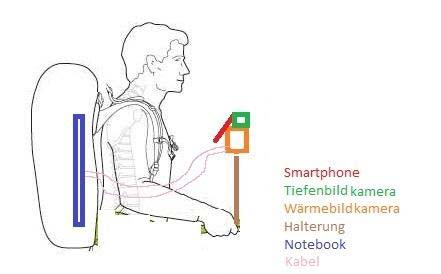
\includegraphics[width=\textwidth]{Study/study1_proto_model.jpg}}{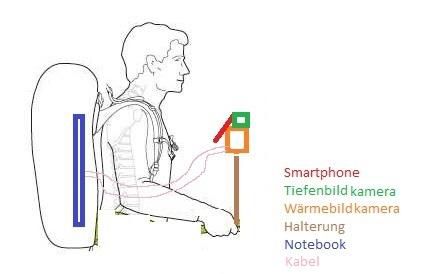
\includegraphics[width=\textwidth]{Study/study1_proto_model.png}}
		\caption{Schematischer Aufbau des Prototyps}
		\label{fig:study1_proto_model}
	\end{subfigure}
	~
	\begin{subfigure}[t]{0.3\textwidth}
		\centering
		\ifthenelse{\boolean{jpg}}{\includegraphics[width=\textwidth]{Study/study1_proto.jpg}}{\includegraphics[width=\textwidth]{Study/study1_proto.png}}
		\caption{Realer Prototyp}
		\label{fig:study1_proto_real}
	\end{subfigure}
	\caption{Benutzte Halterung \& Prototypaufbau}
	\label{fig:study1_proto}
\end{figure}

\begin{figure}[t]
	\begin{subfigure}[t]{0.45\textwidth}
		\centering
		\ifthenelse{\boolean{jpg}}{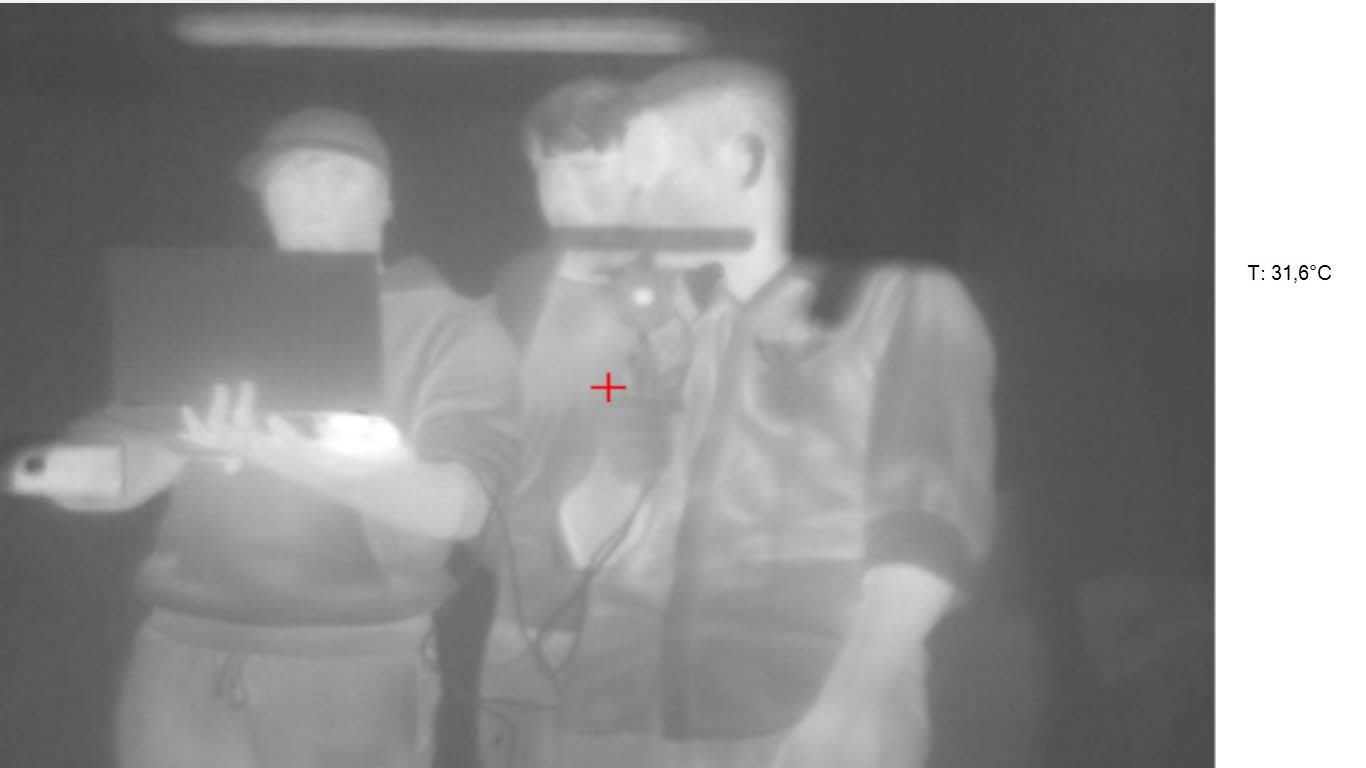
\includegraphics[width=\textwidth]{Study/study1_heat.jpg}}{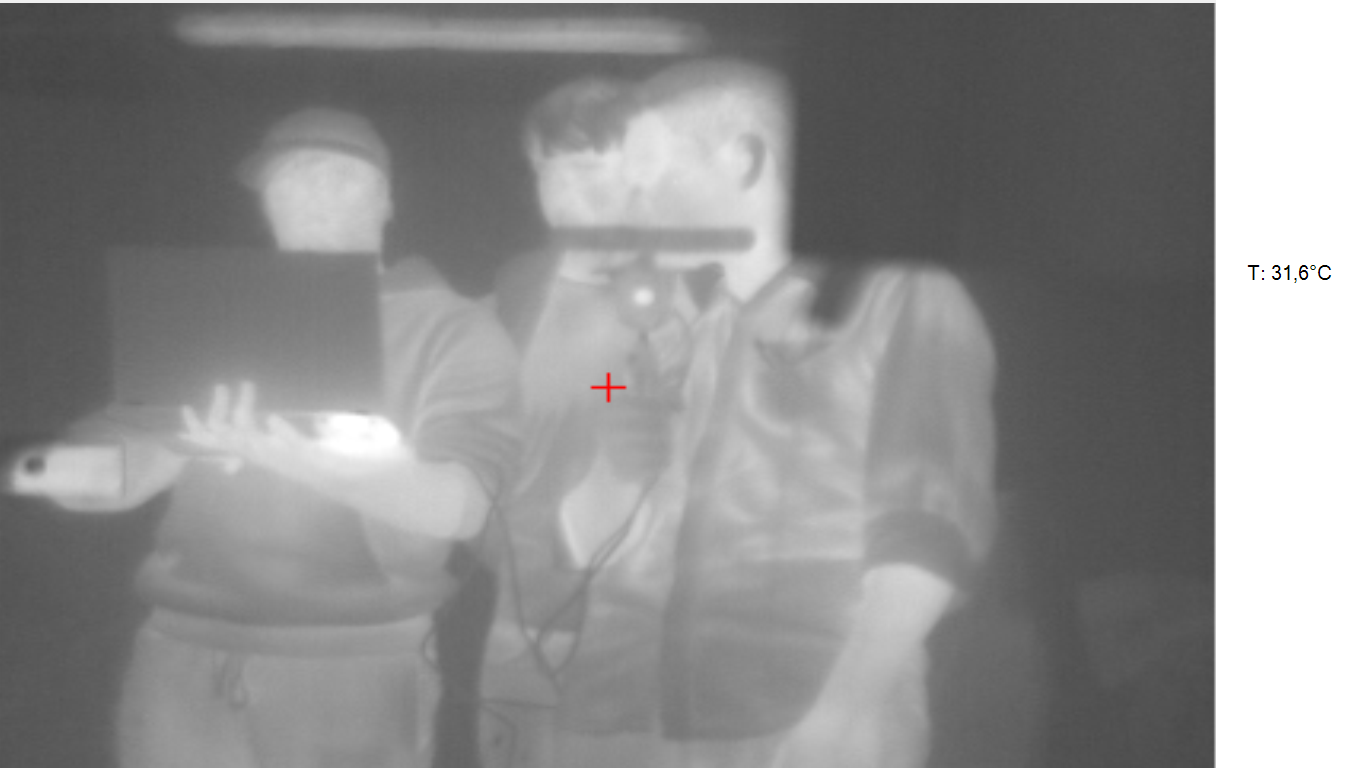
\includegraphics[width=\textwidth]{Study/study1_heat.png}}
		\caption{Wärmebild der Metallplatte}
		\label{fig:study1_heat0}
	\end{subfigure}
	~
	\begin{subfigure}[t]{0.45\textwidth}
		\centering
		\ifthenelse{\boolean{jpg}}{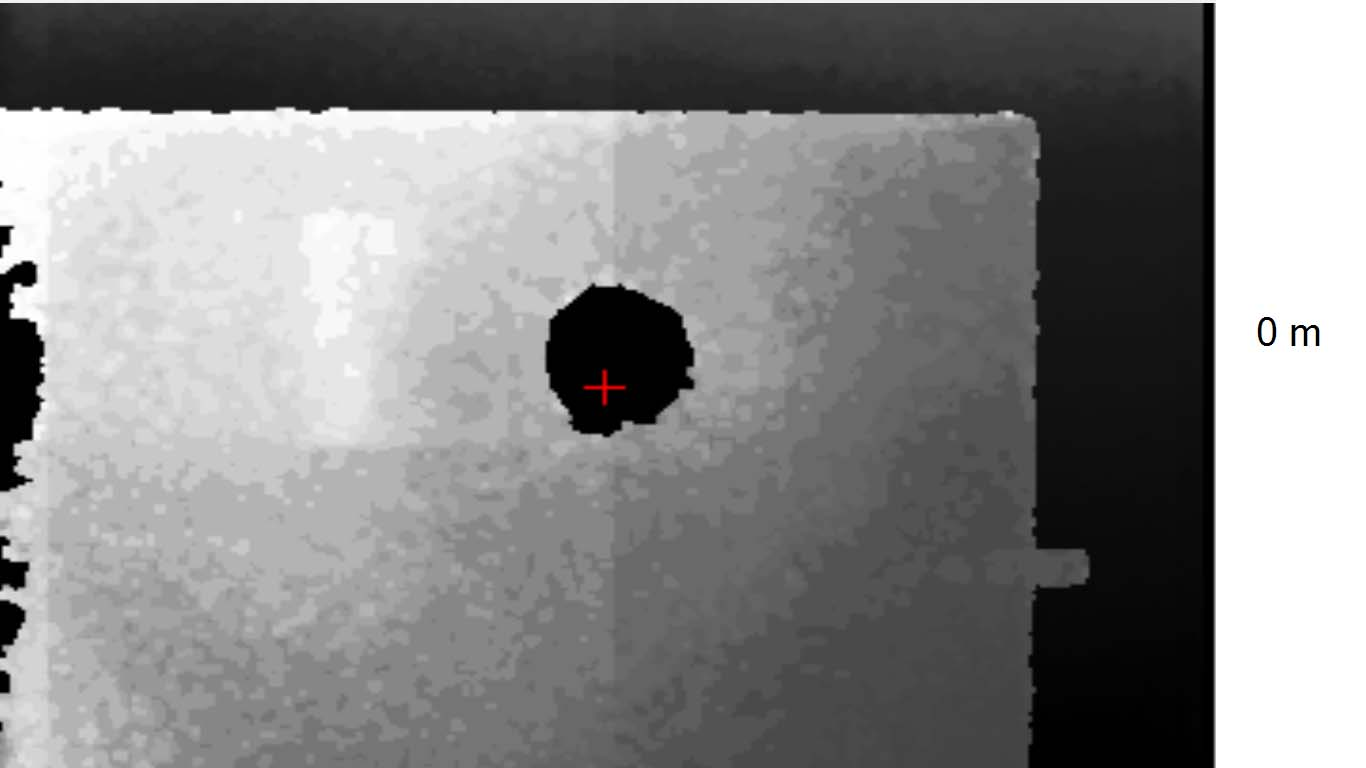
\includegraphics[width=\textwidth]{Study/study1_depth.jpg}}{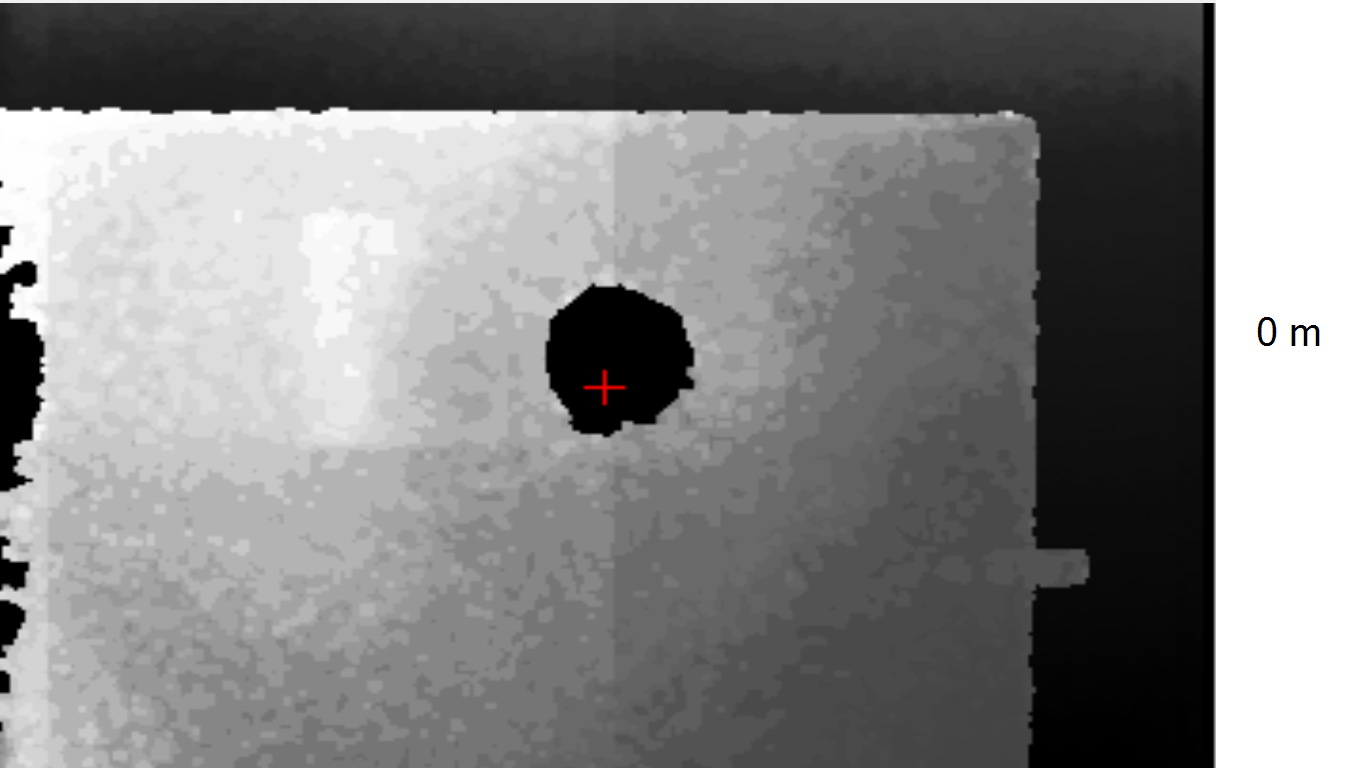
\includegraphics[width=\textwidth]{Study/study1_depth.png}}
		\caption{Tiefenbild der Metallplatte}
		\label{fig:study1_depth0}
	\end{subfigure}
	~
	\begin{subfigure}[t]{0.45\textwidth}
		\centering
		\ifthenelse{\boolean{jpg}}{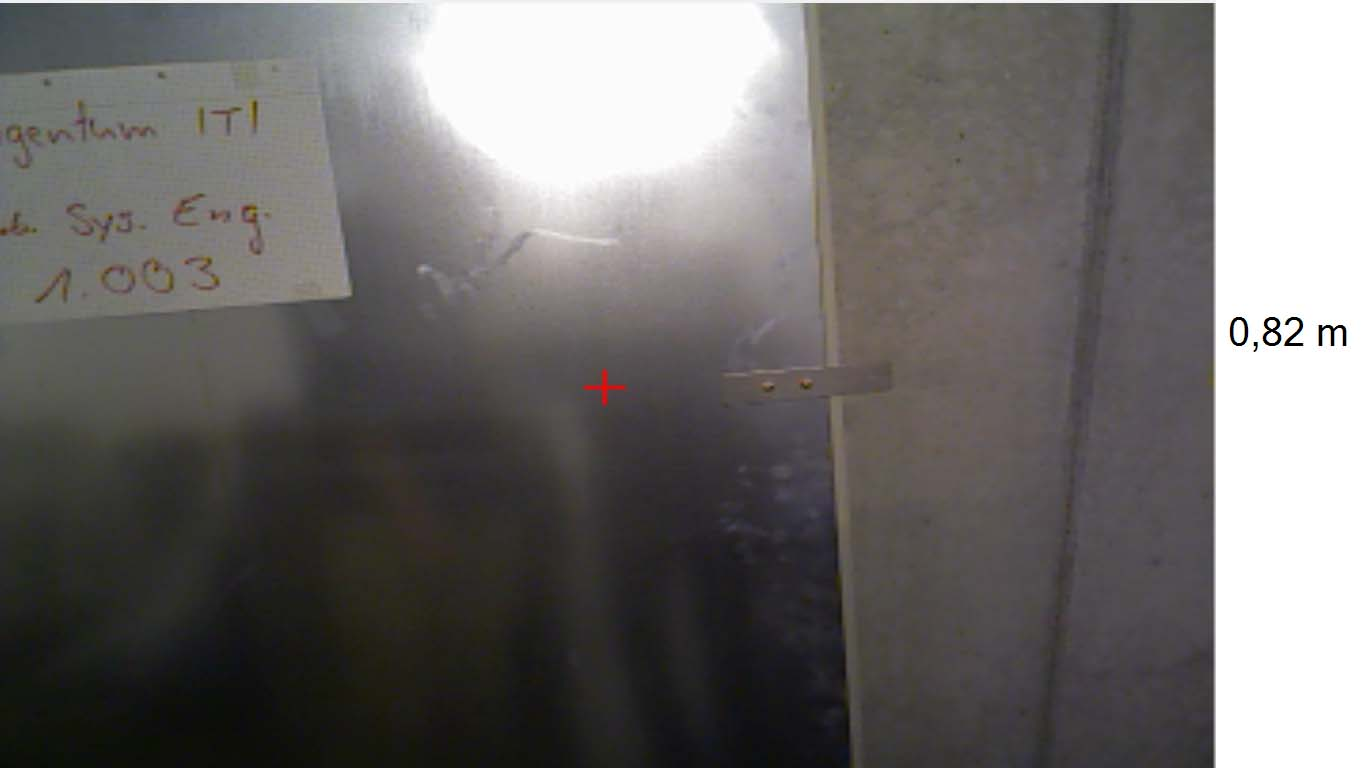
\includegraphics[width=\textwidth]{Study/study1_rgb.jpg}}{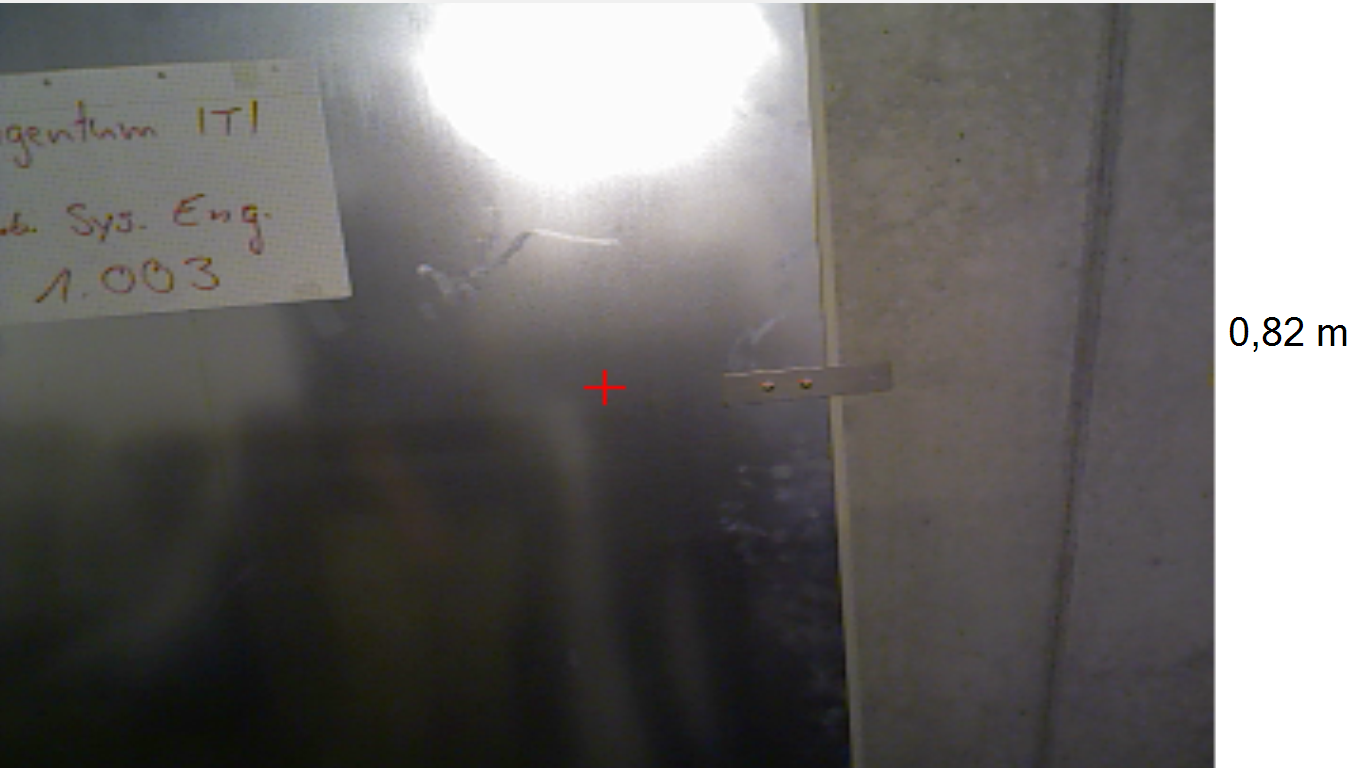
\includegraphics[width=\textwidth]{Study/study1_rgb.png}}
		\caption{RGB-Bild der Metallplatte}
		\label{fig:study1_rgb0}
	\end{subfigure}
	~
	\begin{subfigure}[t]{0.45\textwidth}
		\centering
		\ifthenelse{\boolean{jpg}}{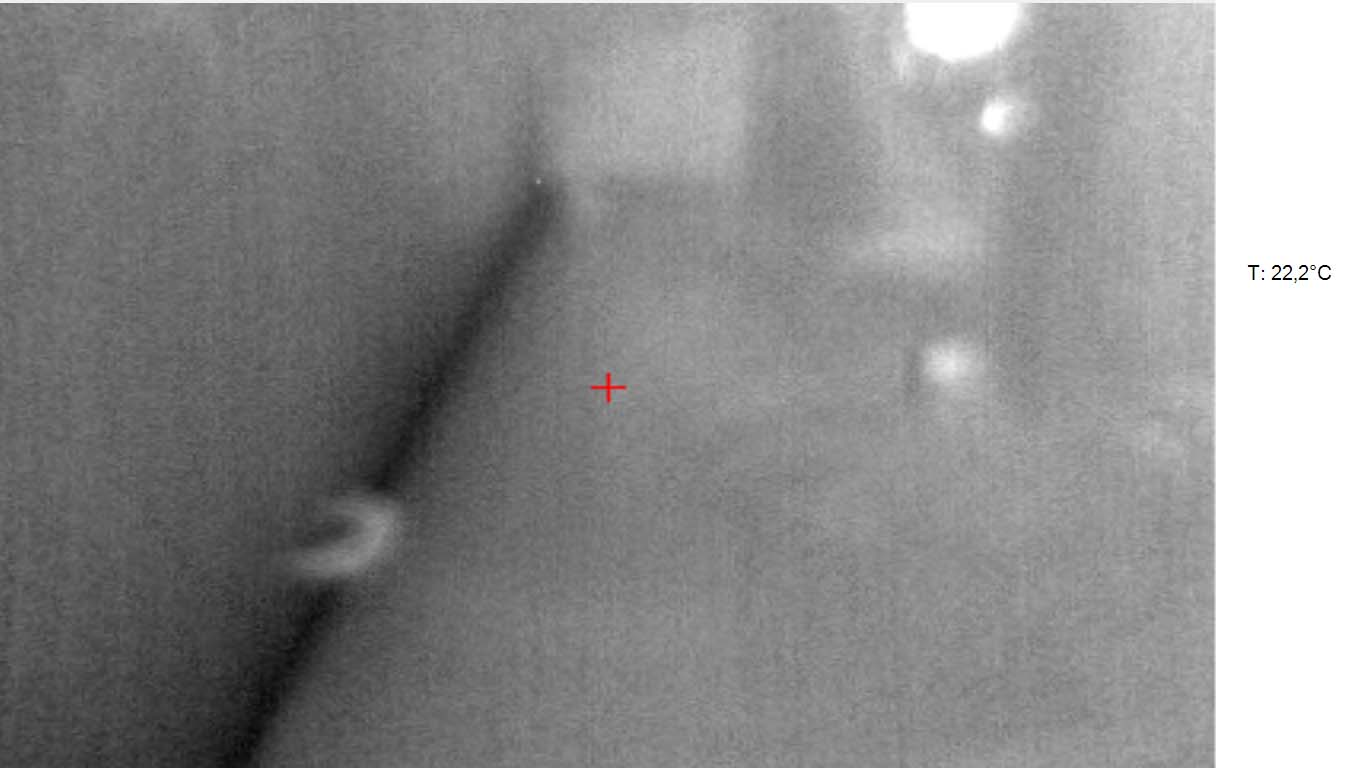
\includegraphics[width=\textwidth]{Study/study1_heat1.jpg}}{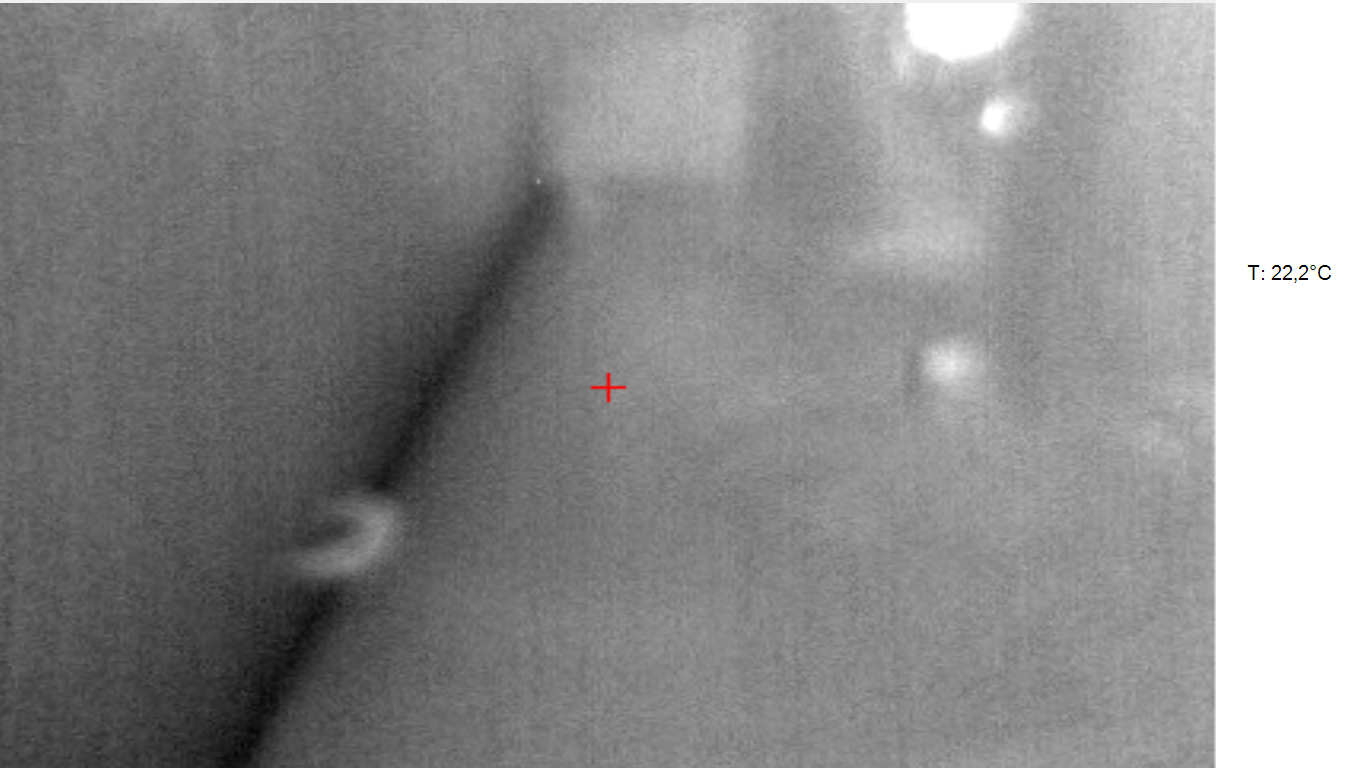
\includegraphics[width=\textwidth]{Study/study1_heat1.png}}
		\caption{Wärmebild des Bodens}
		\label{fig:study1_heat1}
	\end{subfigure}
	~
	\begin{subfigure}[t]{0.45\textwidth}
		\centering
		\ifthenelse{\boolean{jpg}}{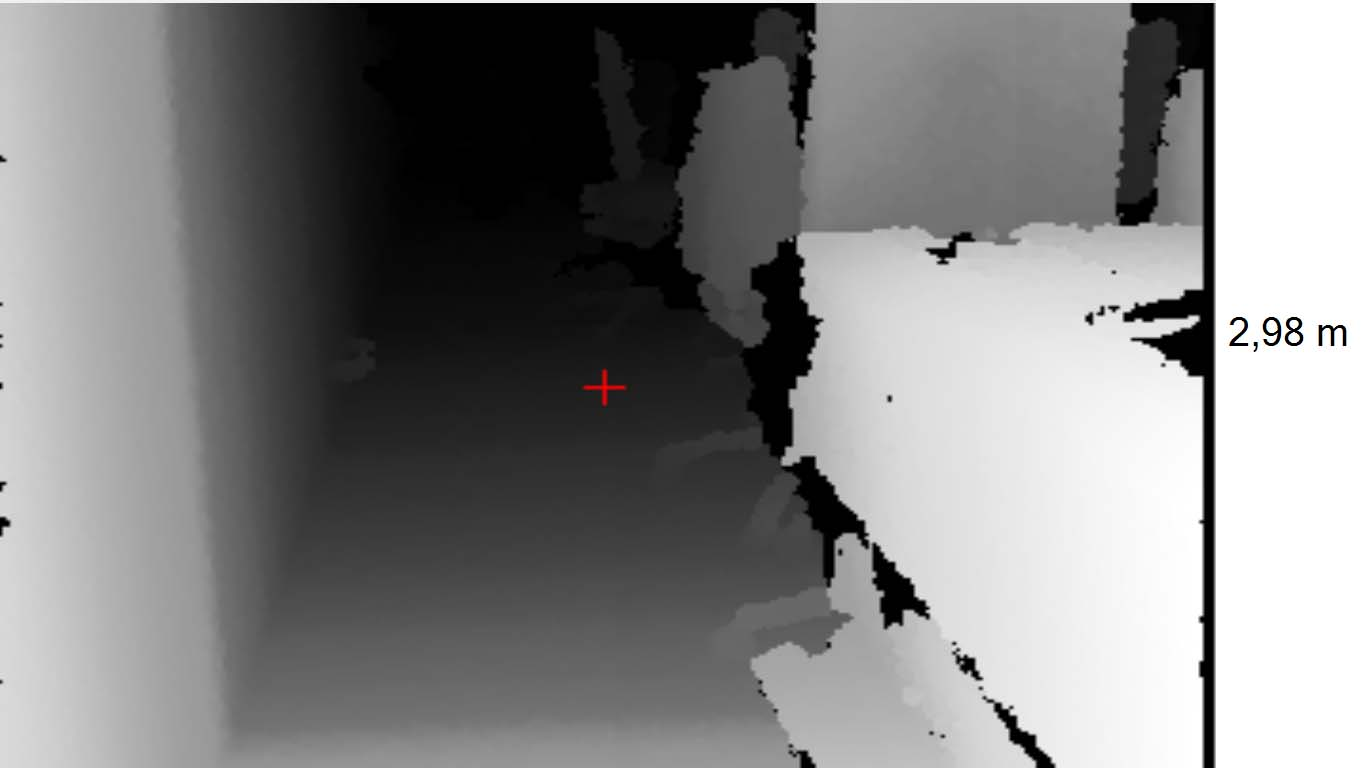
\includegraphics[width=\textwidth]{Study/study1_depth1.jpg}}{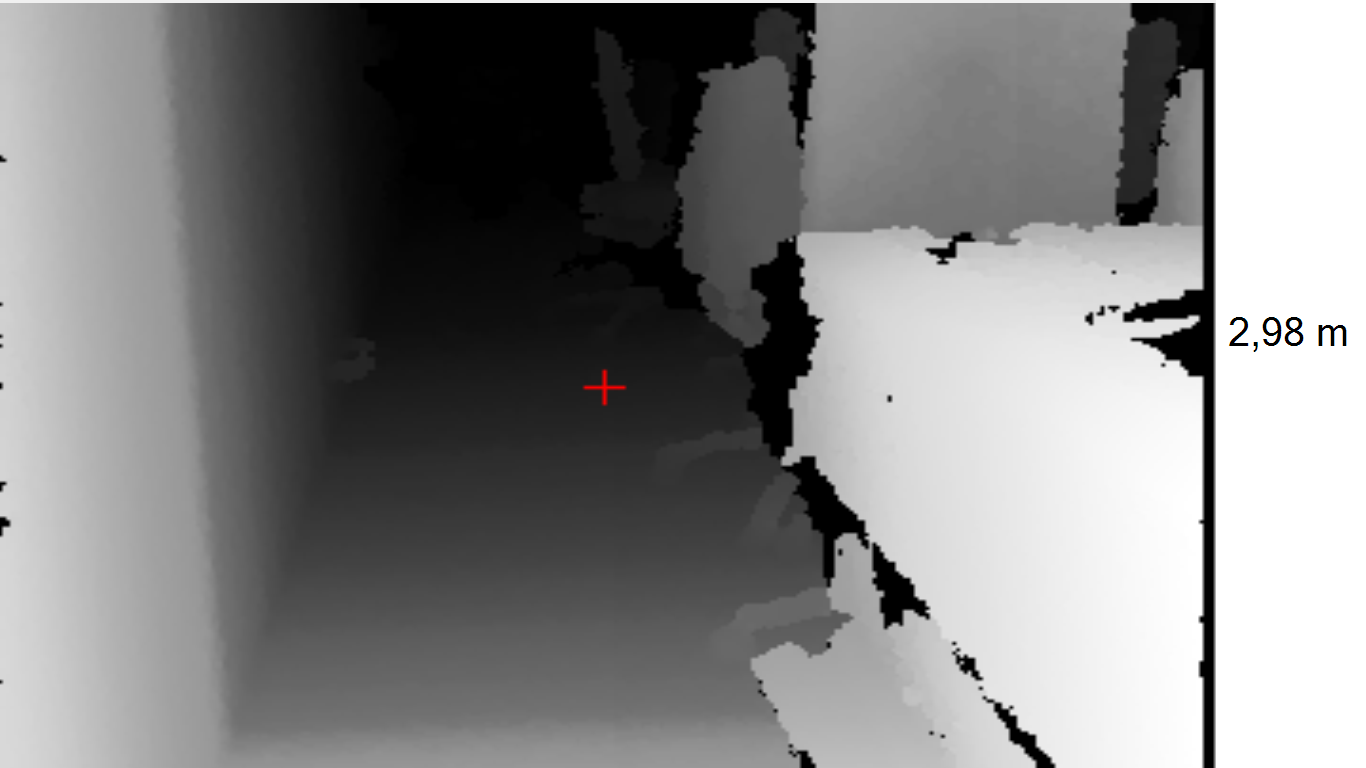
\includegraphics[width=\textwidth]{Study/study1_depth1.png}}
		\caption{Tiefenbild des Bodens}
		\label{fig:study1_depth1}
	\end{subfigure}
	~
	\begin{subfigure}[t]{0.45\textwidth}
		\centering
		\ifthenelse{\boolean{jpg}}{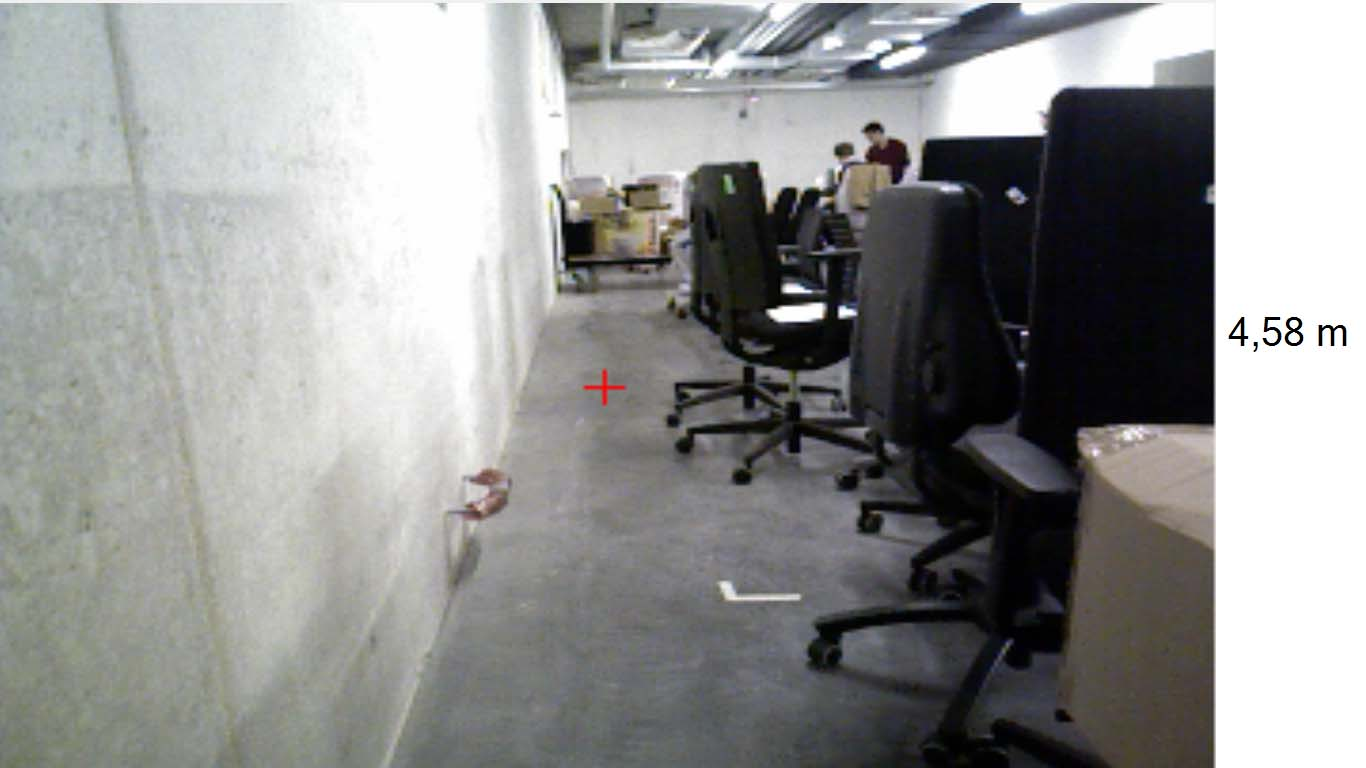
\includegraphics[width=\textwidth]{Study/study1_rgb1.jpg}}{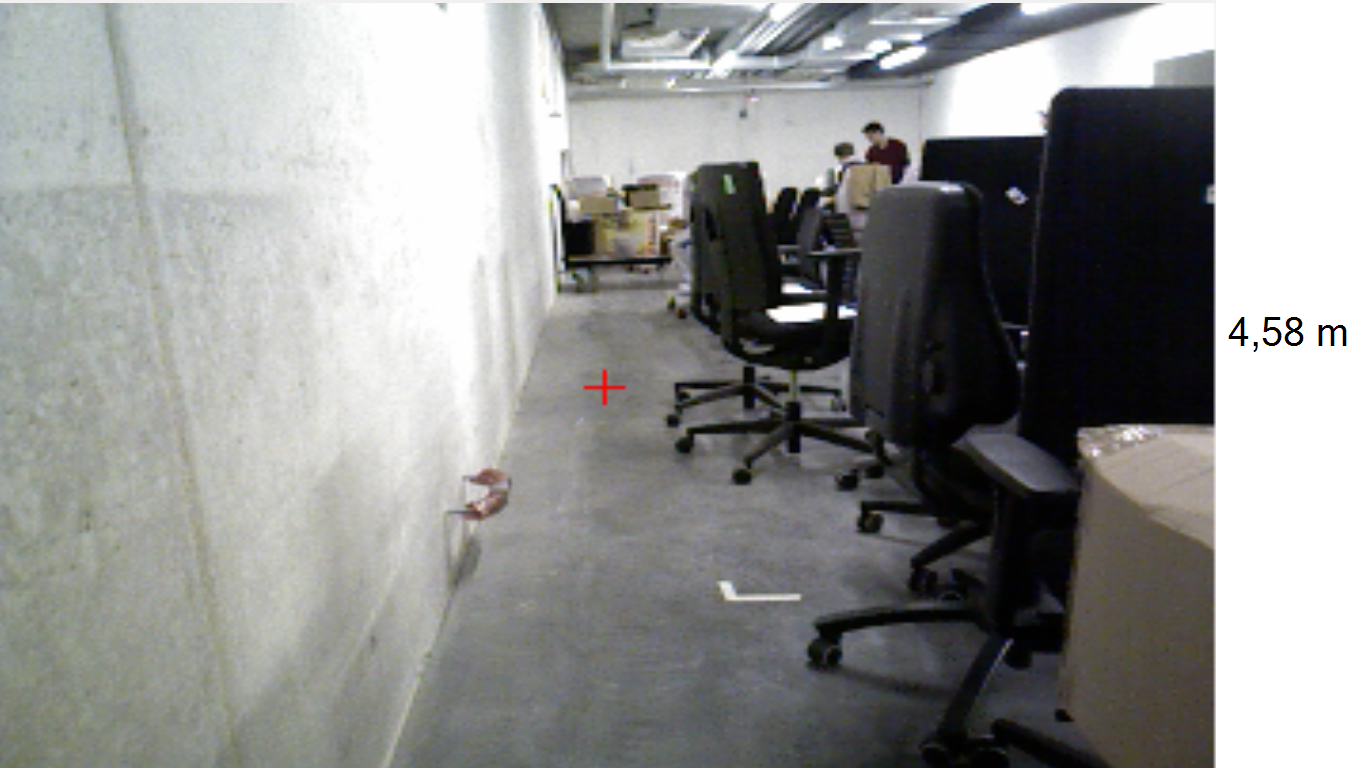
\includegraphics[width=\textwidth]{Study/study1_rgb1.png}}
		\caption{RGB-Bild des Bodens}
		\label{fig:study1_rgb1}
	\end{subfigure}
	\caption{Wärme-, Tiefen- und RGB-Bilder des Aufbaus}
	\label{fig:study1_modes}
\end{figure}

\begin{figure}[t]
	\centering
	\begin{subfigure}[t]{0.45\textwidth}
		\centering
		\ifthenelse{\boolean{jpg}}{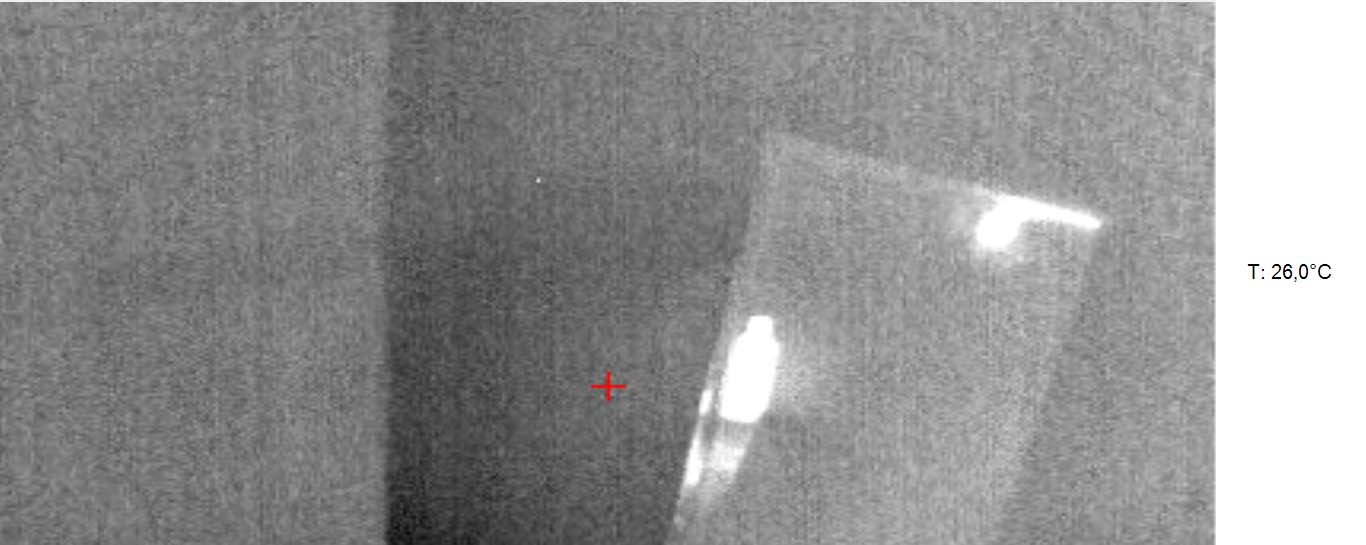
\includegraphics[width=\textwidth]{Study/study1_heat2.jpg}}{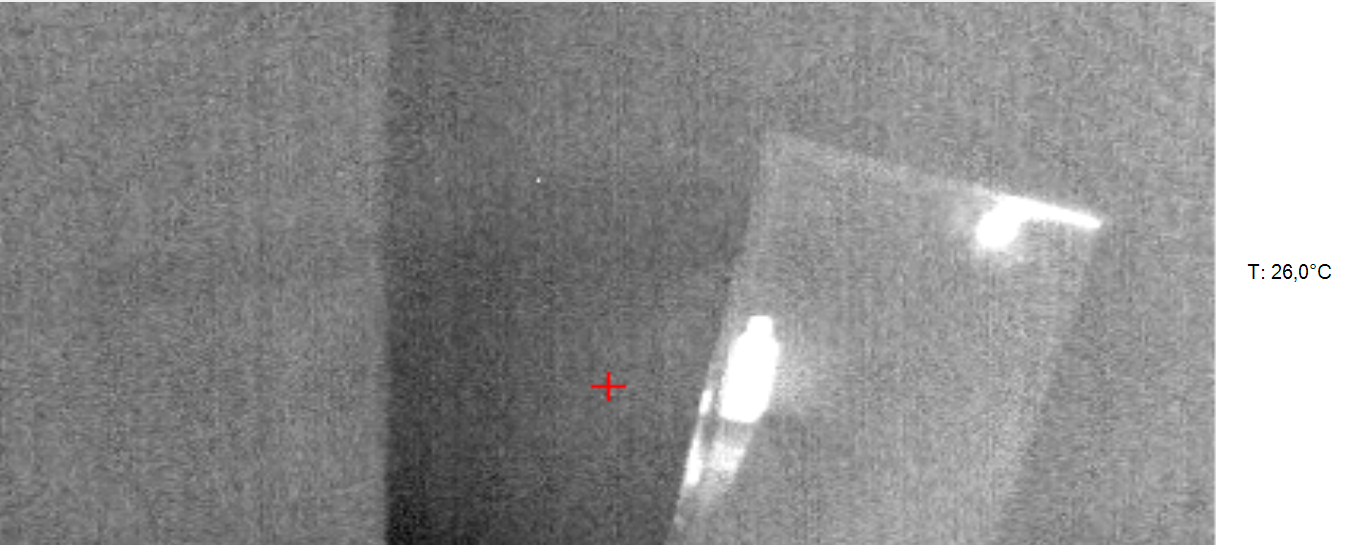
\includegraphics[width=\textwidth]{Study/study1_heat2.png}}
		\caption{Wärmebild des Spiegels}
		\label{fig:study1_heat2}
	\end{subfigure}
	~
	\begin{subfigure}[t]{0.45\textwidth}
		\centering
		\ifthenelse{\boolean{jpg}}{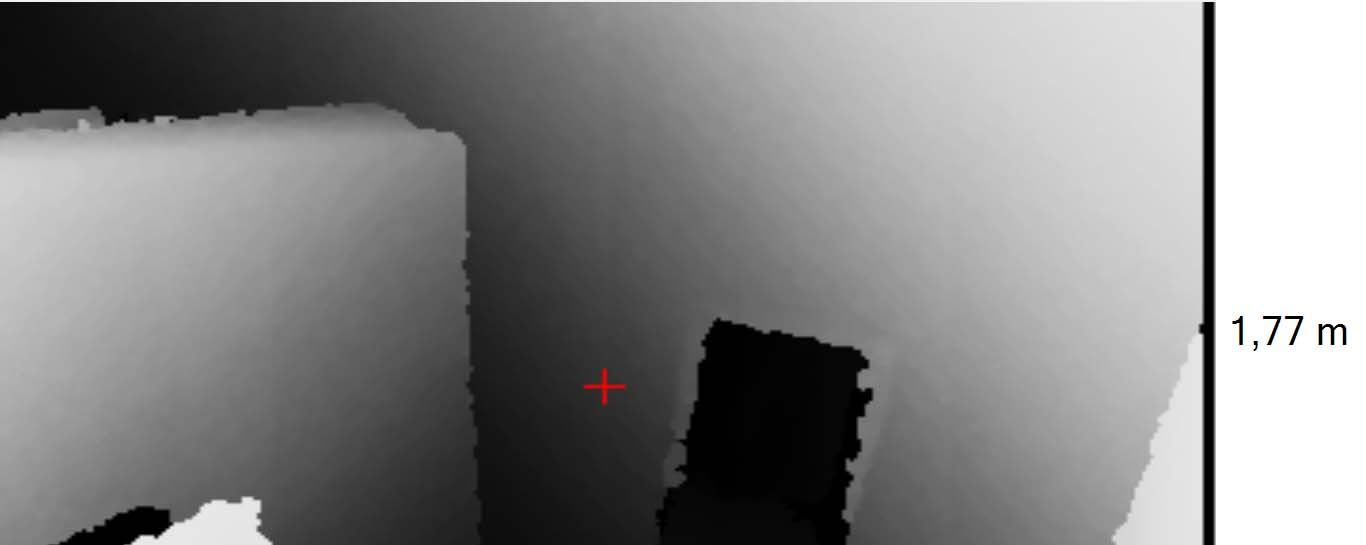
\includegraphics[width=\textwidth]{Study/study1_depth2.jpg}}{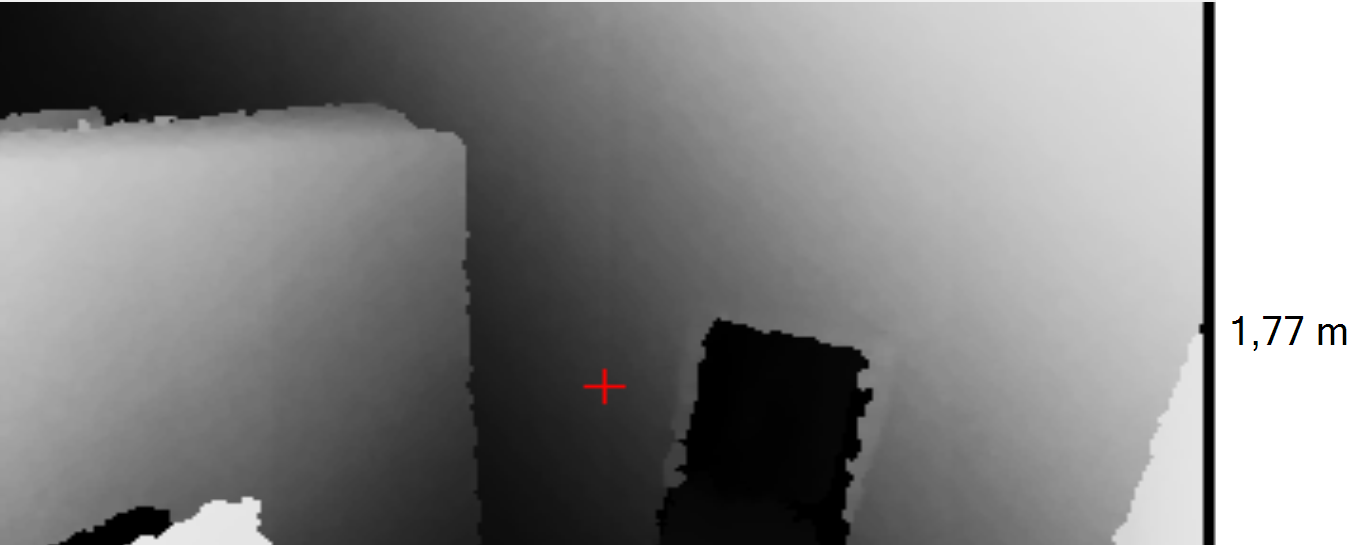
\includegraphics[width=\textwidth]{Study/study1_depth2.png}}
		\caption{Tiefenbild des Spiegels}
		\label{fig:study1_depth2}
	\end{subfigure}
	~
	\begin{subfigure}[t]{0.45\textwidth}
		\centering
		\ifthenelse{\boolean{jpg}}{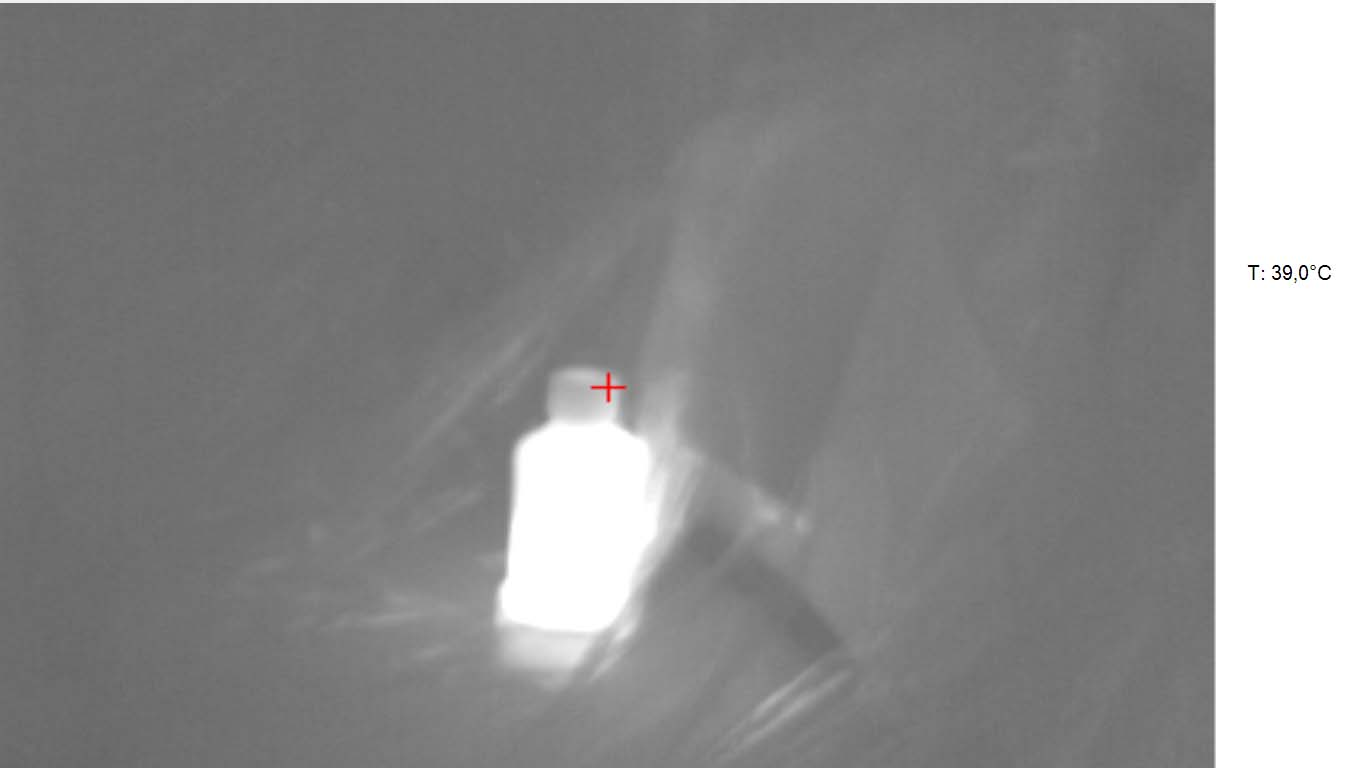
\includegraphics[width=\textwidth]{Study/study1_heat3.jpg}}{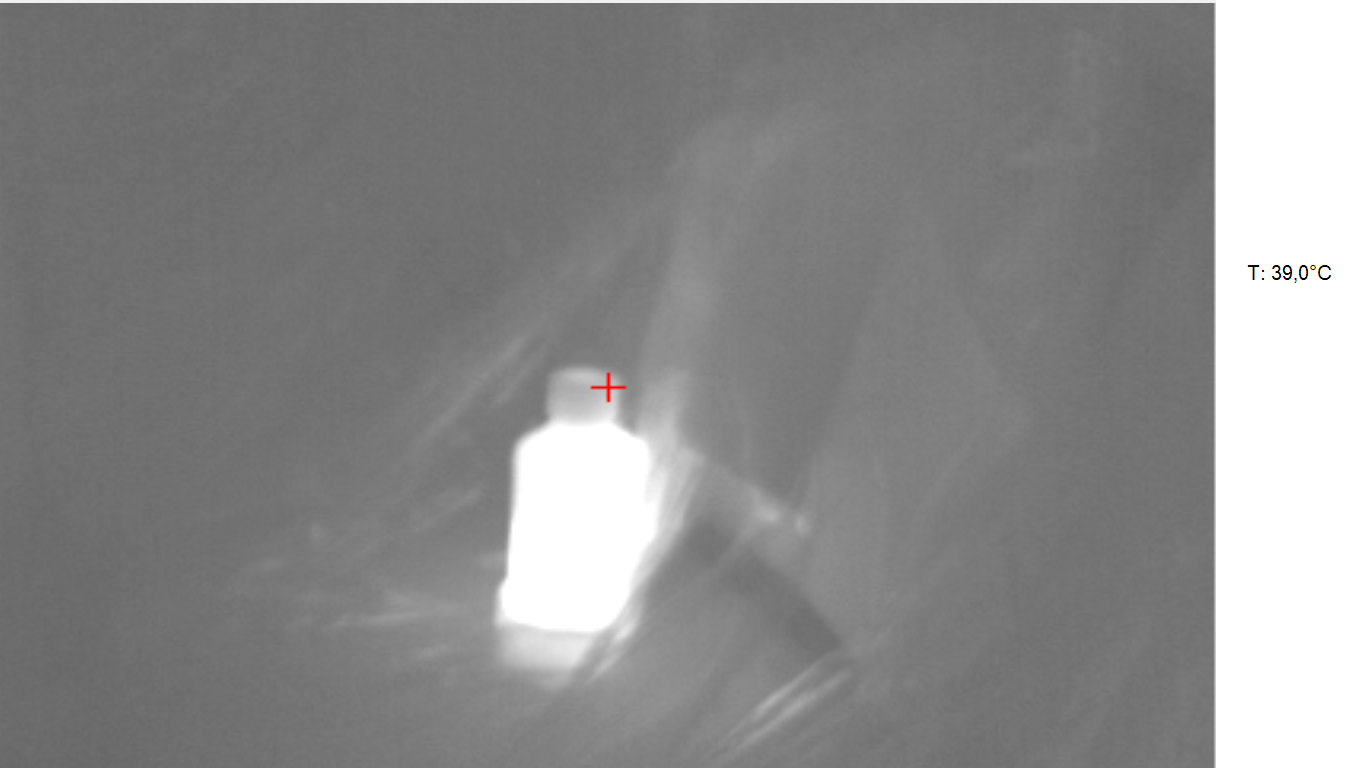
\includegraphics[width=\textwidth]{Study/study1_heat3.png}}
		\caption{Wärmebild einer versteckten Flasche}
		\label{fig:study1_heat3}
	\end{subfigure}
	~
	\begin{subfigure}[t]{0.45\textwidth}
		\centering
		\ifthenelse{\boolean{jpg}}{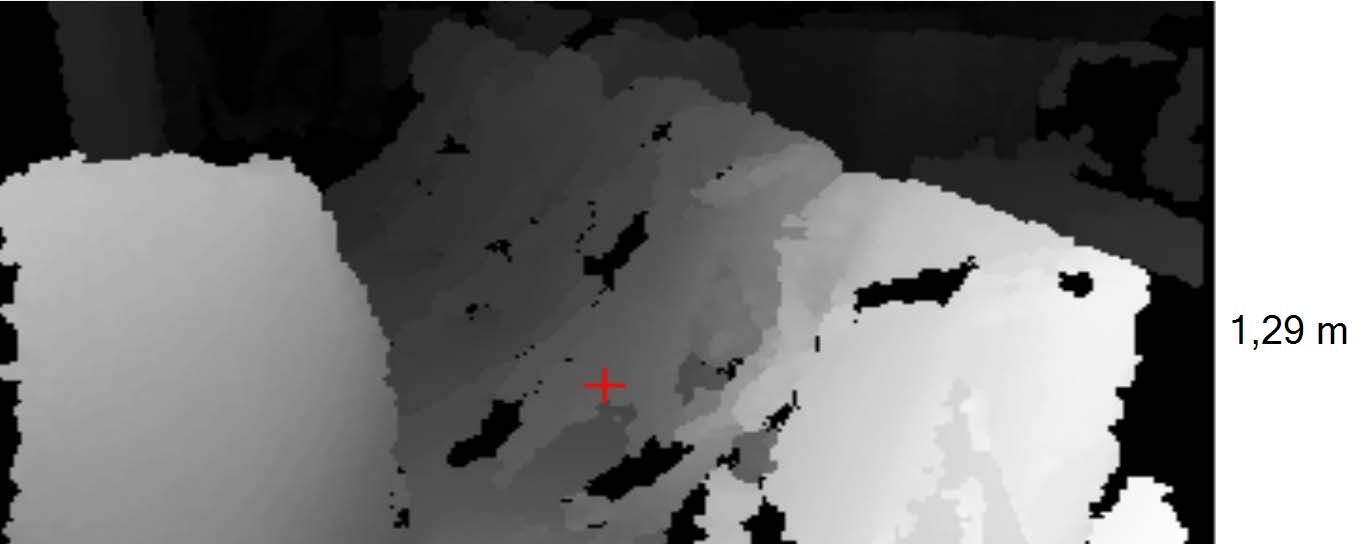
\includegraphics[width=\textwidth]{Study/study1_depth3.jpg}}{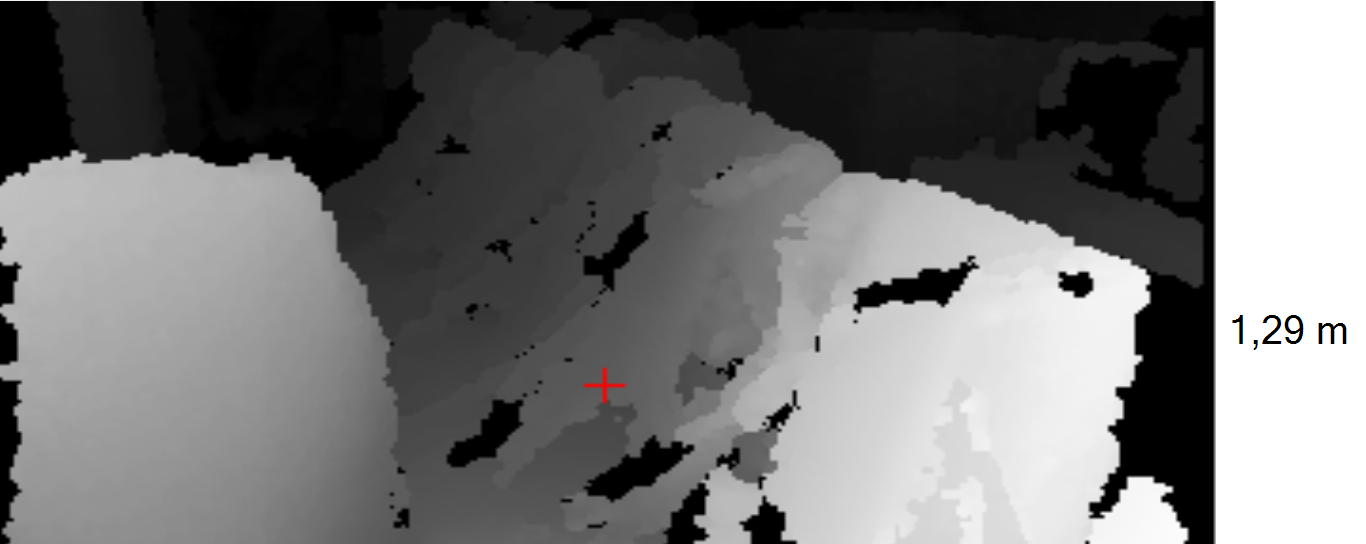
\includegraphics[width=\textwidth]{Study/study1_depth3.png}}
		\caption{Tiefenbild einer versteckten Flasche}
		\label{fig:study1_depth3}
	\end{subfigure}
	~
	\begin{subfigure}[t]{0.45\textwidth}
		\centering
		\ifthenelse{\boolean{jpg}}{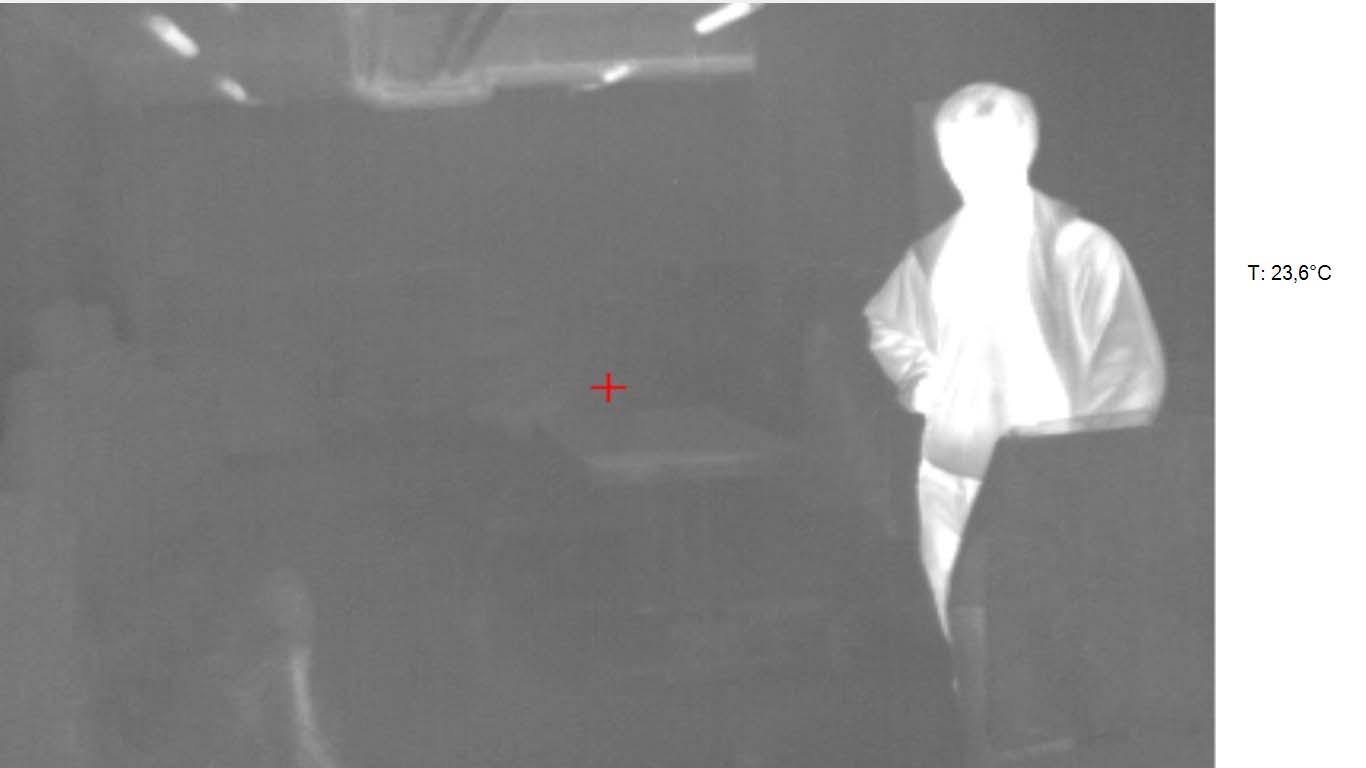
\includegraphics[width=\textwidth]{Study/study1_heat4.jpg}}{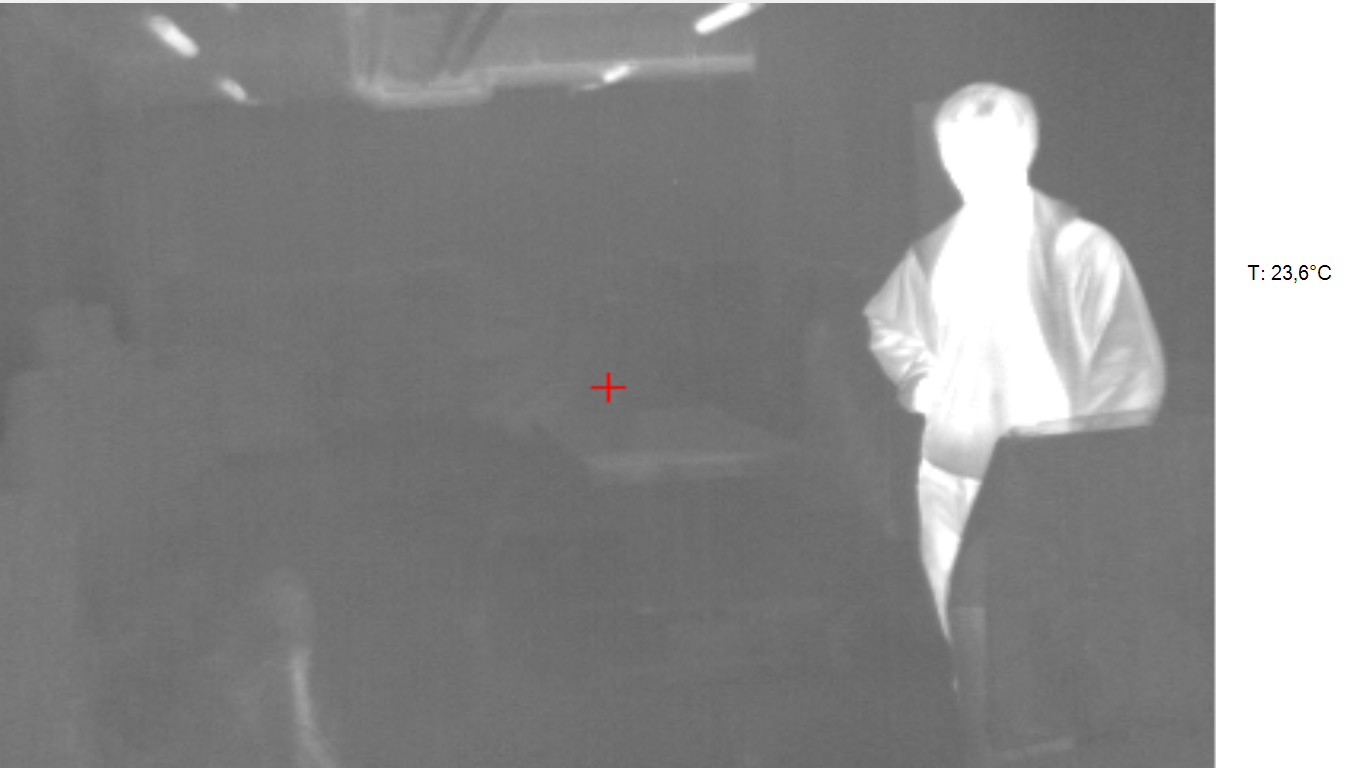
\includegraphics[width=\textwidth]{Study/study1_heat4.png}}
		\caption{Wärmebild des Bodens}
		\label{fig:study1_heat4}
	\end{subfigure}
	~
	\begin{subfigure}[t]{0.45\textwidth}
		\centering
		\ifthenelse{\boolean{jpg}}{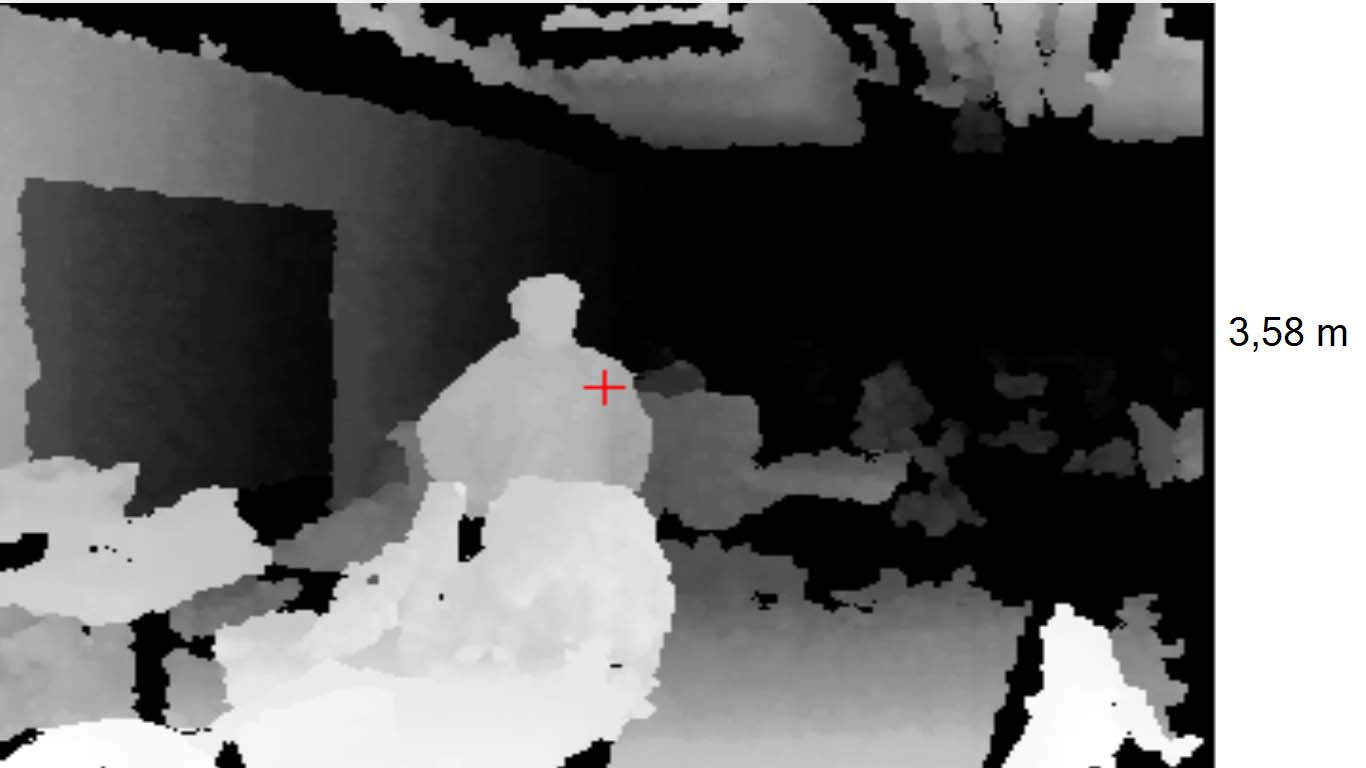
\includegraphics[width=\textwidth]{Study/study1_depth4.jpg}}{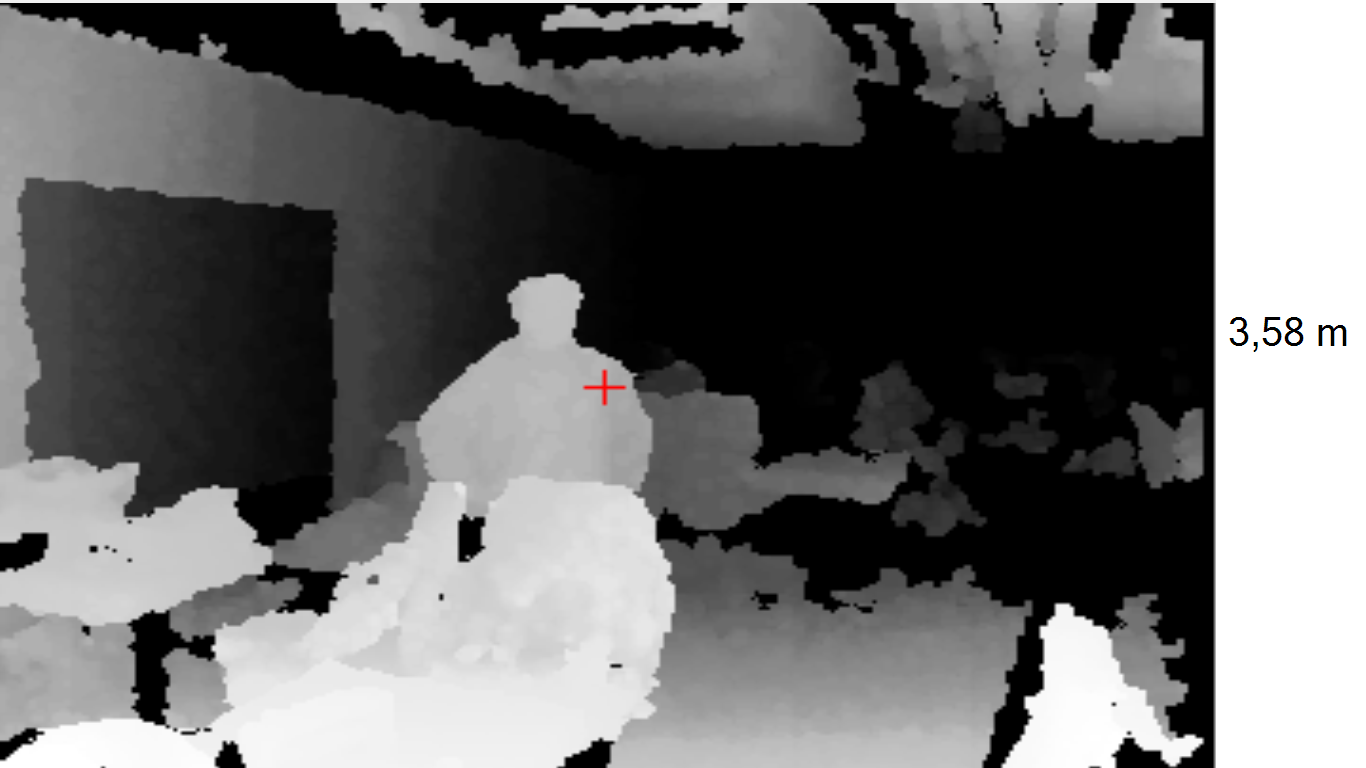
\includegraphics[width=\textwidth]{Study/study1_depth4.png}}
		\caption{Tiefenbild des Raums}
		\label{fig:study1_depth4}
	\end{subfigure}
	~
	\begin{subfigure}[t]{0.45\textwidth}
		\centering
		\ifthenelse{\boolean{jpg}}{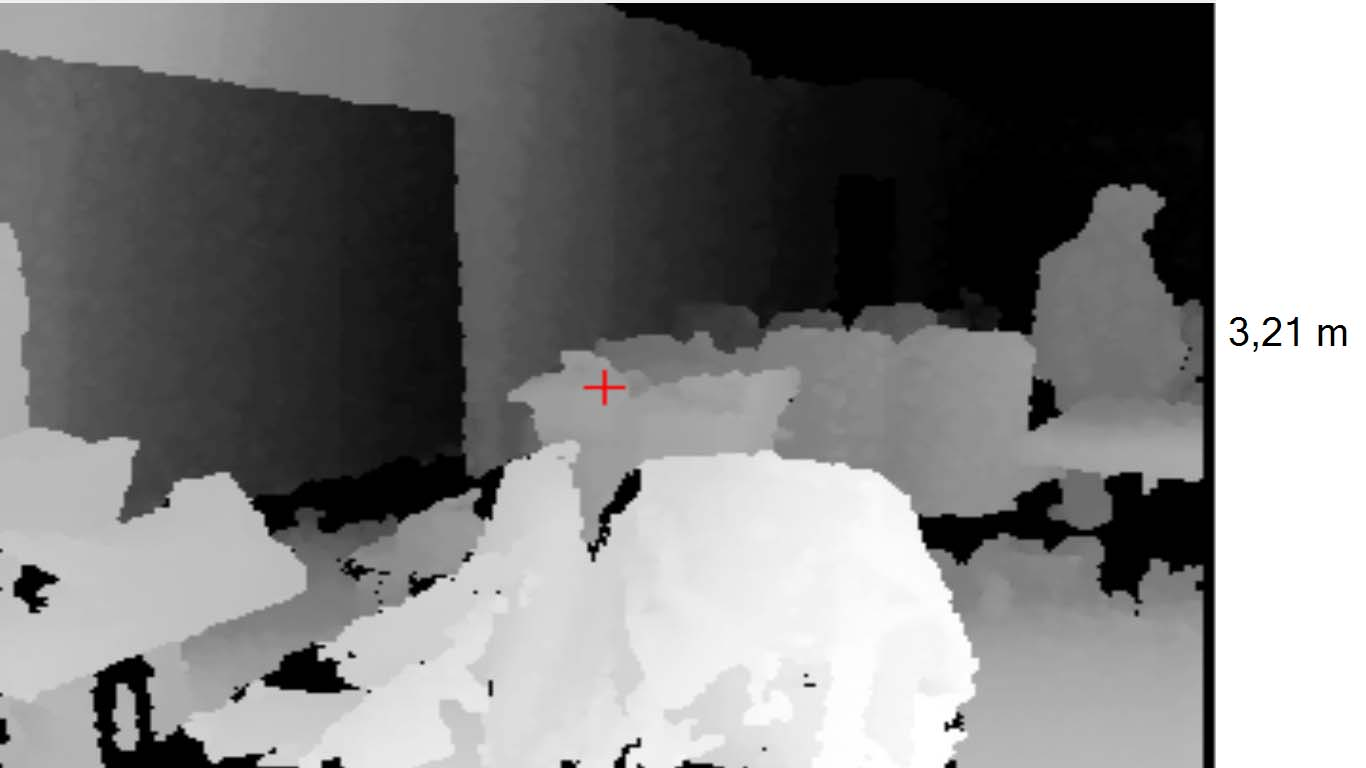
\includegraphics[width=\textwidth]{Study/study1_depth5.jpg}}{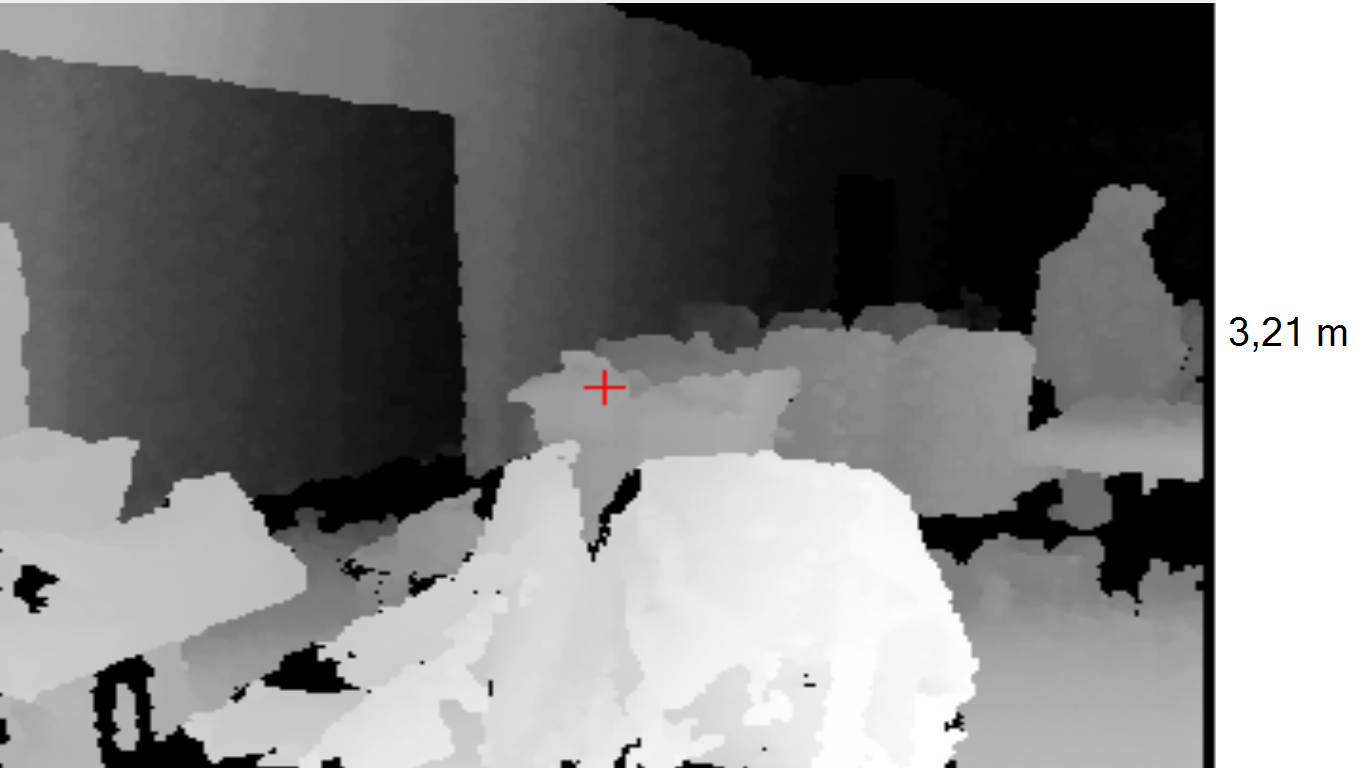
\includegraphics[width=\textwidth]{Study/study1_depth5.png}}
		\caption{Tiefenbild des Raums}
		\label{fig:study1_depth5}
	\end{subfigure}
	\caption{Wärme- und Tiefenbilder des Aufbaus der ersten Studie}
	\label{fig:study1_modes1}
\end{figure}
 
Als erstes wurden die Probanden in den, ihnen unbekannten, Nebenraum des abgedunkelten Kellers geführt.
In diesem, in \cref{fig:study1_room} dargestellten, Raum durften sie sich für maximal 30 Sekunden frei in der Nähe des Eingangs bewegen und mussten dann Angaben zu Länge und Breite machen.
Darauf wurden die Teilnehmer in einen anderen Raum geführt, in welchem das Labyrinth aus \cref{fig:study1_labyrinth} mit mehreren Hindernissen aufgebaut war.
Der Aufbau des Labyrinths bestand aus Stühlen, Tischen und Kartons, wobei die Teilnehmer darauf hingewiesen wurden, dass sie diese nicht verstellen oder überklettern dürfen.
Dabei war die Aufgabe eine mit heißem Wasser gefüllte Wärmeflasche zu finden und zum Eingang zu bringen.
Zu den Hindernissen zählten zwei spiegelnde Objekte, ein Spiegel und eine Metallplatte, und vier normale Flaschen, welche auch mit heißem Wasser gefühlt waren.
In \cref{fig:study1_lab} sind Bilder des Aufbaus enthalten.

Dabei wurde sowohl die benötigte Dauer, bis die Flasche zurückgebracht, sowie wie lange welcher Modus genutzt wurde gemessen.
Zusätzlich wurde die Ausgabe aufgenommen.
Der ganze Verlauf wurde von zwei Infrarotkameras aufgezeichnet und gleichzeitig darüber überwacht.

\subsubsection{Das Interview}
Nachdem der Proband die Wärmeflasche zurückgebracht hatte, wurde ein Interview mit selbigen durchgeführt.
Dabei wurden unter anderem diverse Metadaten, bisherige Erfahrung mit Wärme- wie Tiefenbildkameras, sowie Beurteilungen des Prototypen und Testlaufs festgehalten.

\begin{figure}[H]
	\centering
	\begin{subfigure}[t]{0.65\textwidth}
		\centering
		\ifthenelse{\boolean{jpg}}{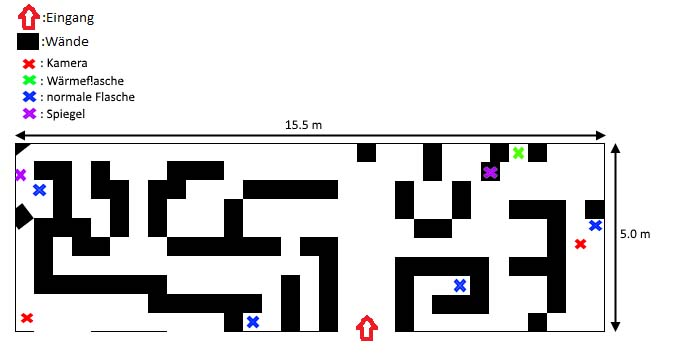
\includegraphics[width=\textwidth]{Study/study1_labyrinth.jpg}}{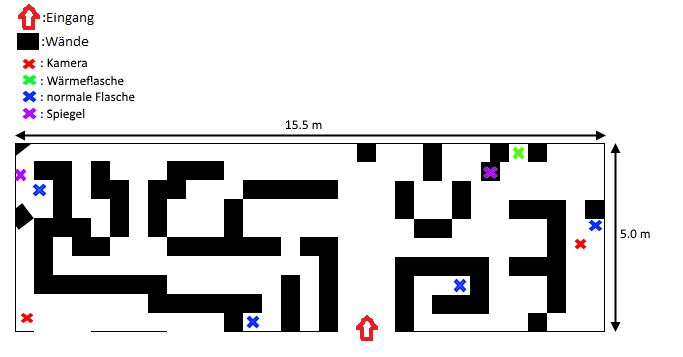
\includegraphics[width=\textwidth]{Study/study1_labyrinth.png}}
		\caption{Schematischer Labyrinthaufbau}
		\label{fig:study1_labyrinth}
	\end{subfigure}
	~
	\begin{subfigure}[t]{0.3\textwidth}
		\centering
		\ifthenelse{\boolean{jpg}}{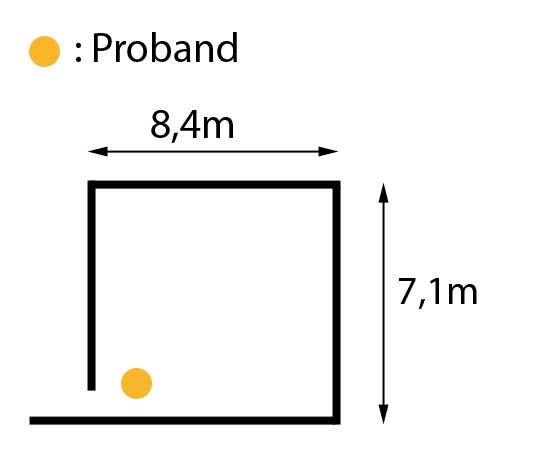
\includegraphics[width=\textwidth]{Study/study1_nebenraum.jpg}}{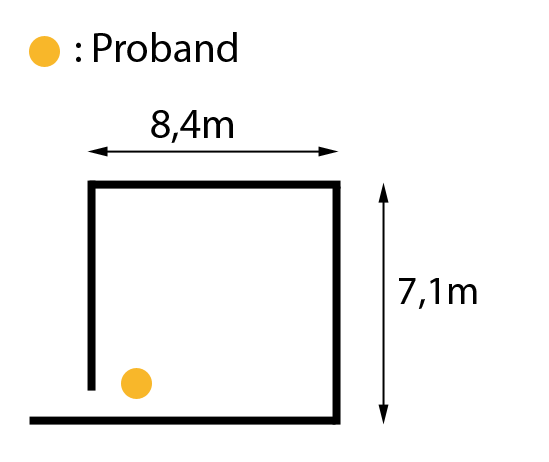
\includegraphics[width=\textwidth]{Study/study1_nebenraum.png}}
		\caption{Schematischer Nebenraum}
		\label{fig:study1_room}
	\end{subfigure}
	\caption{Studienorte}
	\label{fig:study1_keller}
\end{figure}

\begin{figure}[t]
	\begin{subfigure}[t]{0.3\textwidth}
		\centering
		\ifthenelse{\boolean{jpg}}{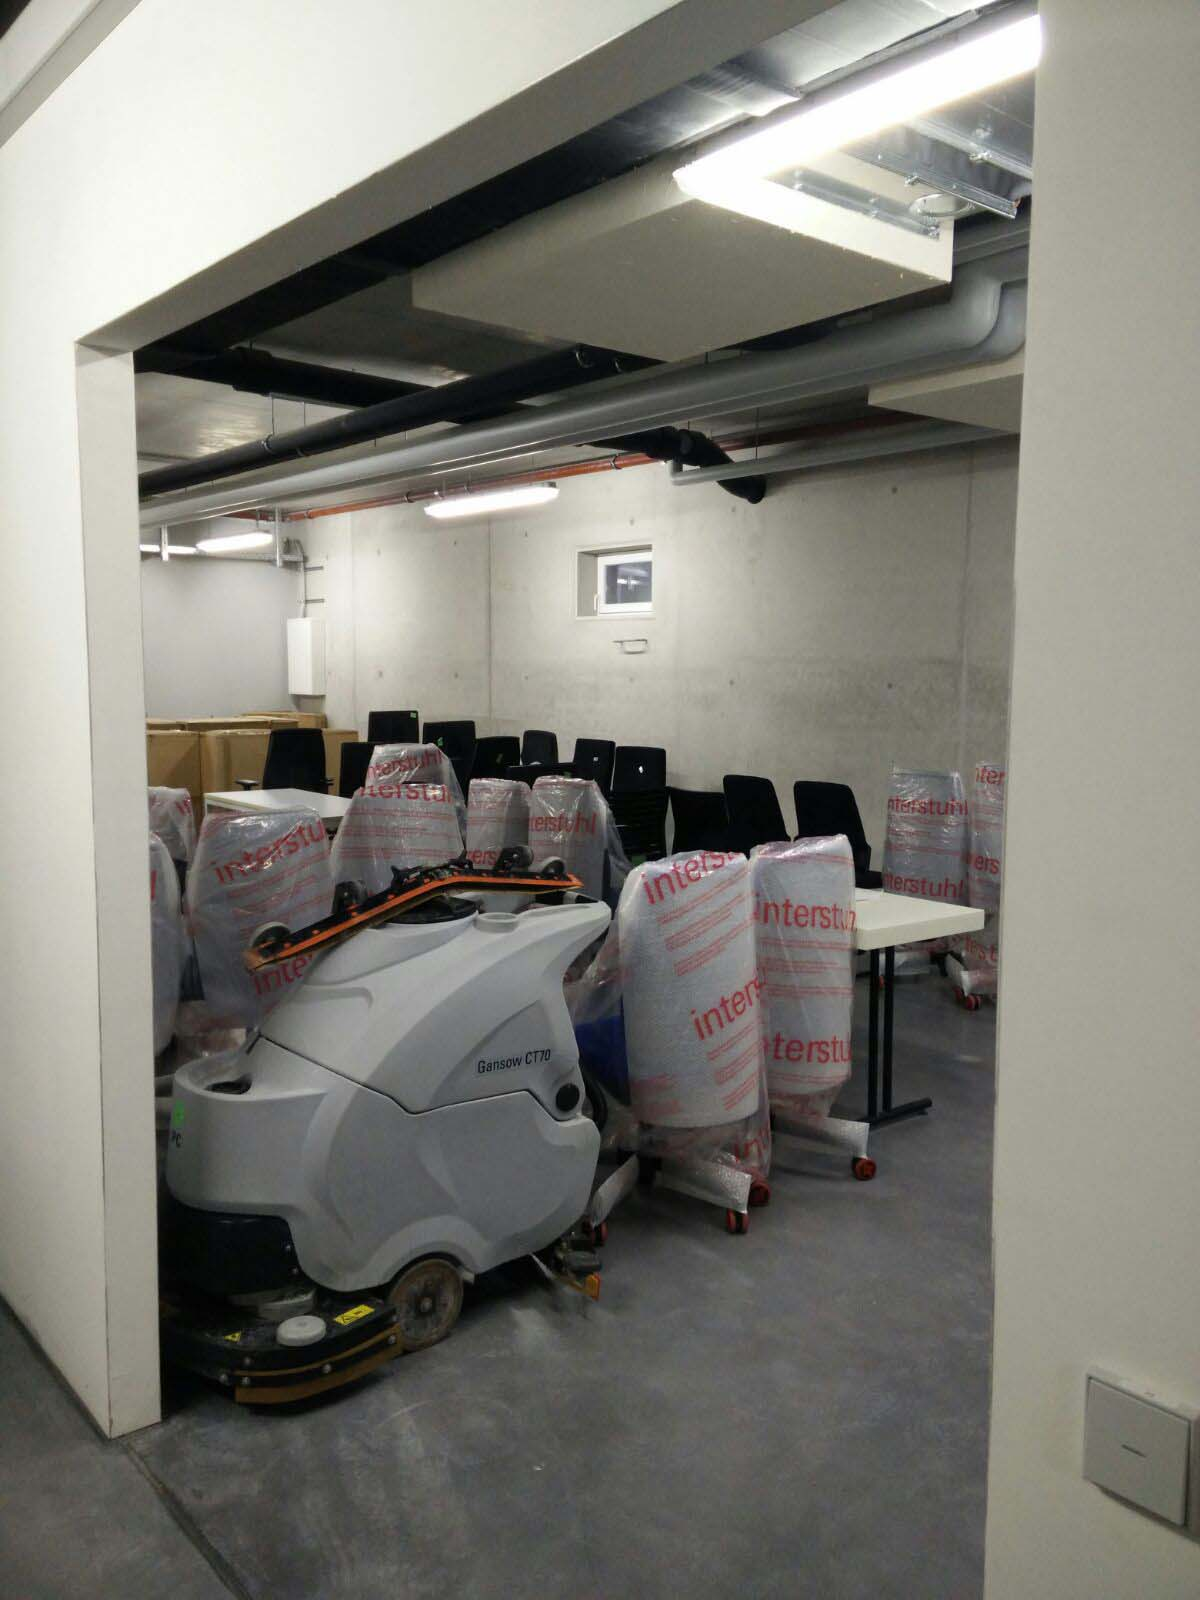
\includegraphics[width=\textwidth]{Study/study1_1_Walkin_In.jpg}}{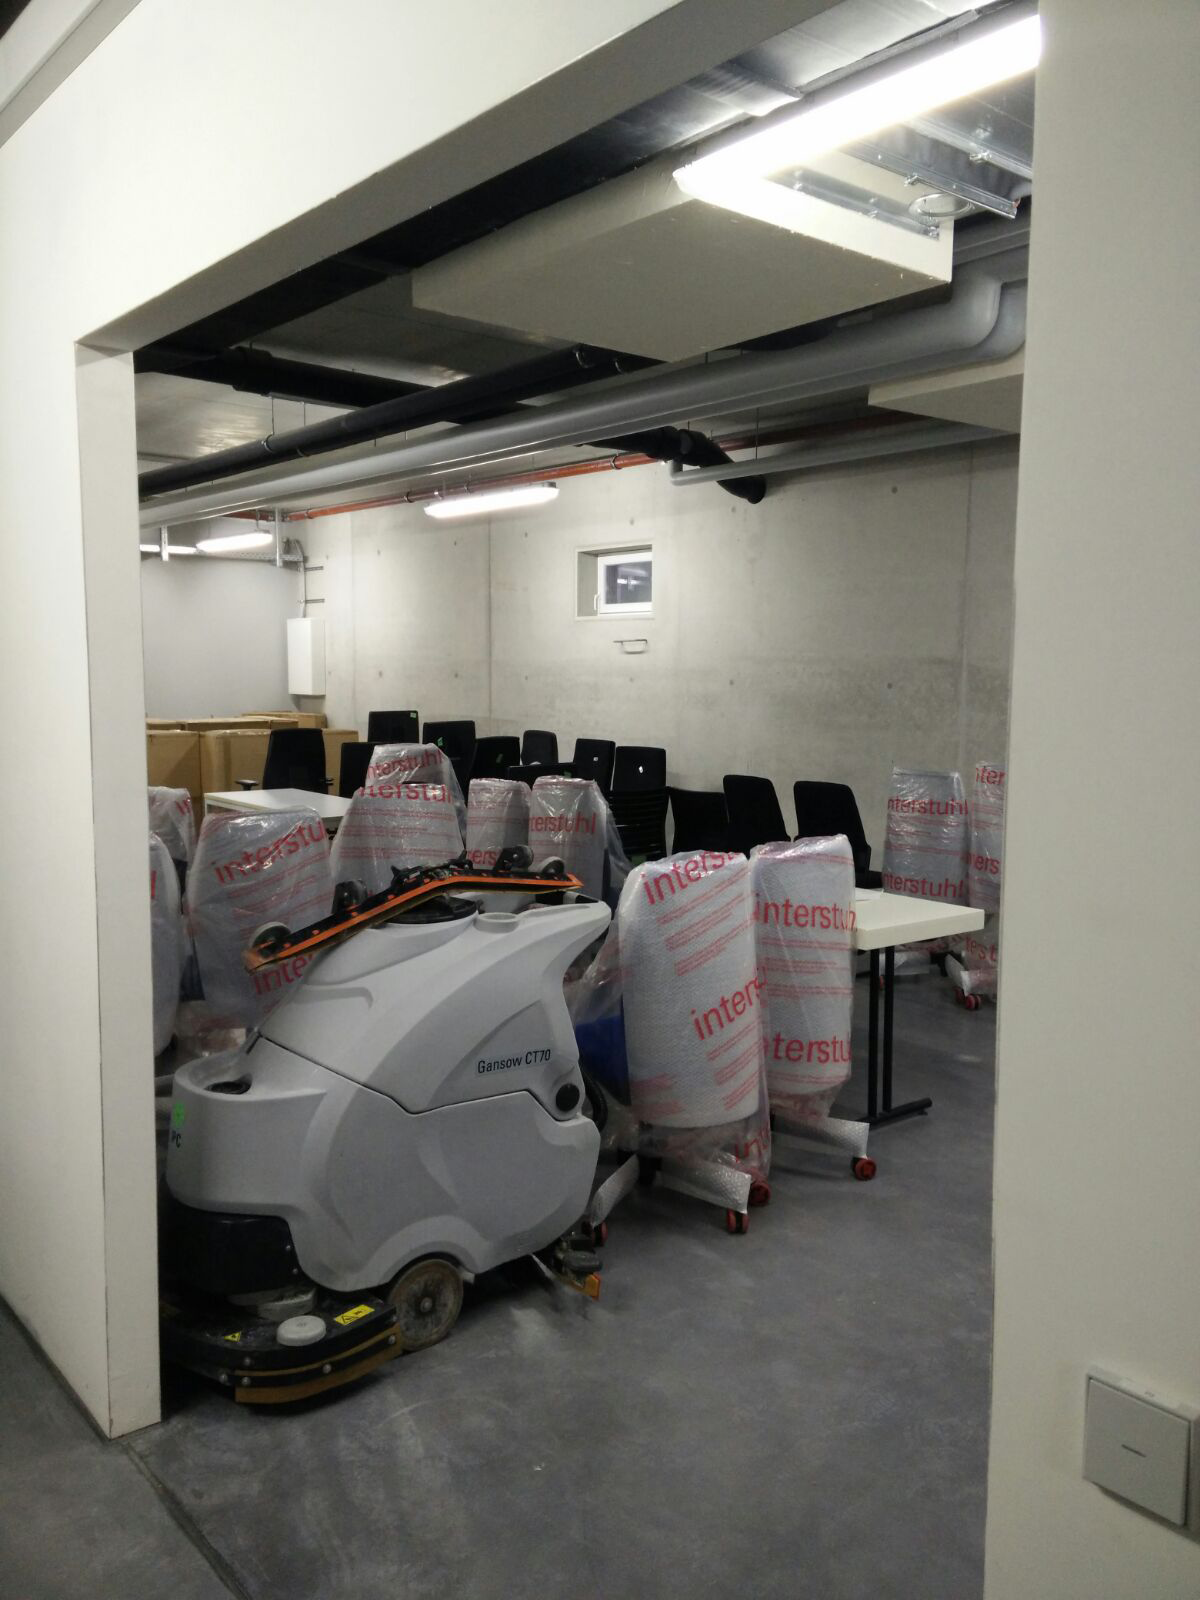
\includegraphics[width=\textwidth]{Study/study1_1_Walkin_In.png}}
		\caption{Labyrintheingang}
		\label{fig:study1_lab1}
	\end{subfigure}
	~
	\begin{subfigure}[t]{0.3\textwidth}
		\centering
		\ifthenelse{\boolean{jpg}}{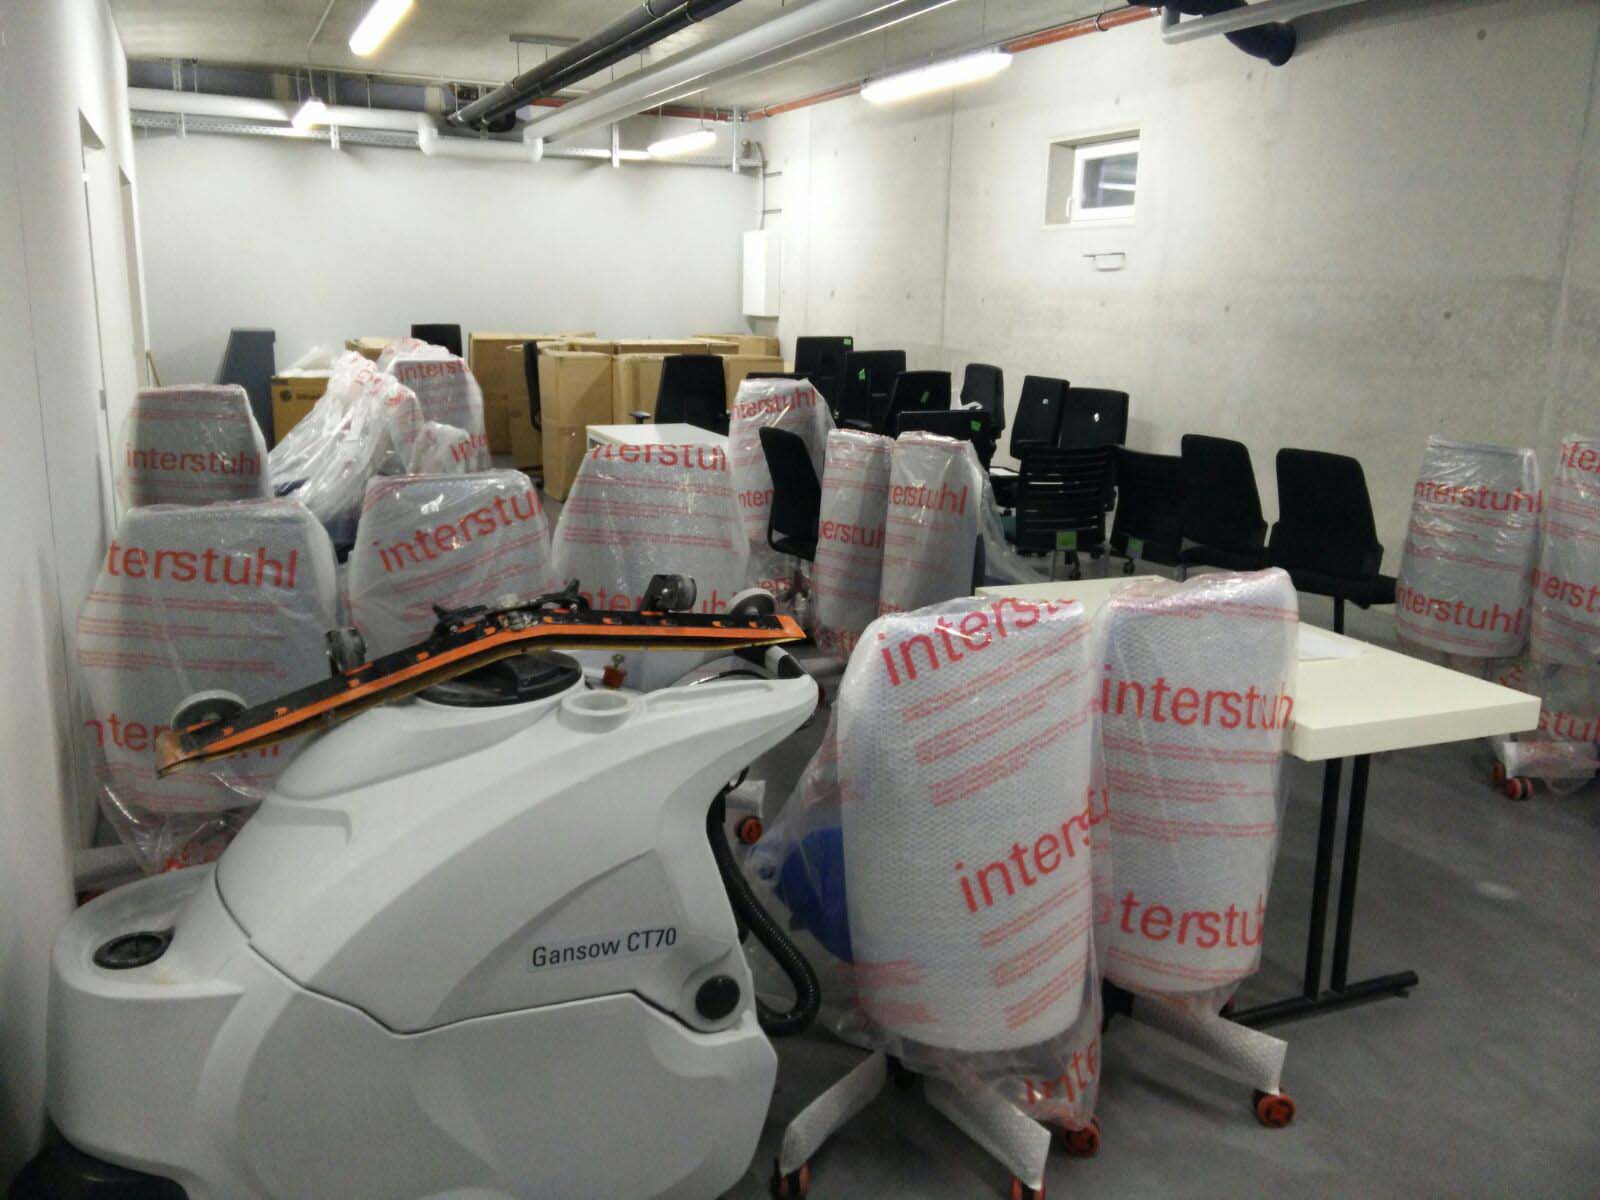
\includegraphics[width=\textwidth]{Study/study1_2_Close_Left.jpg}}{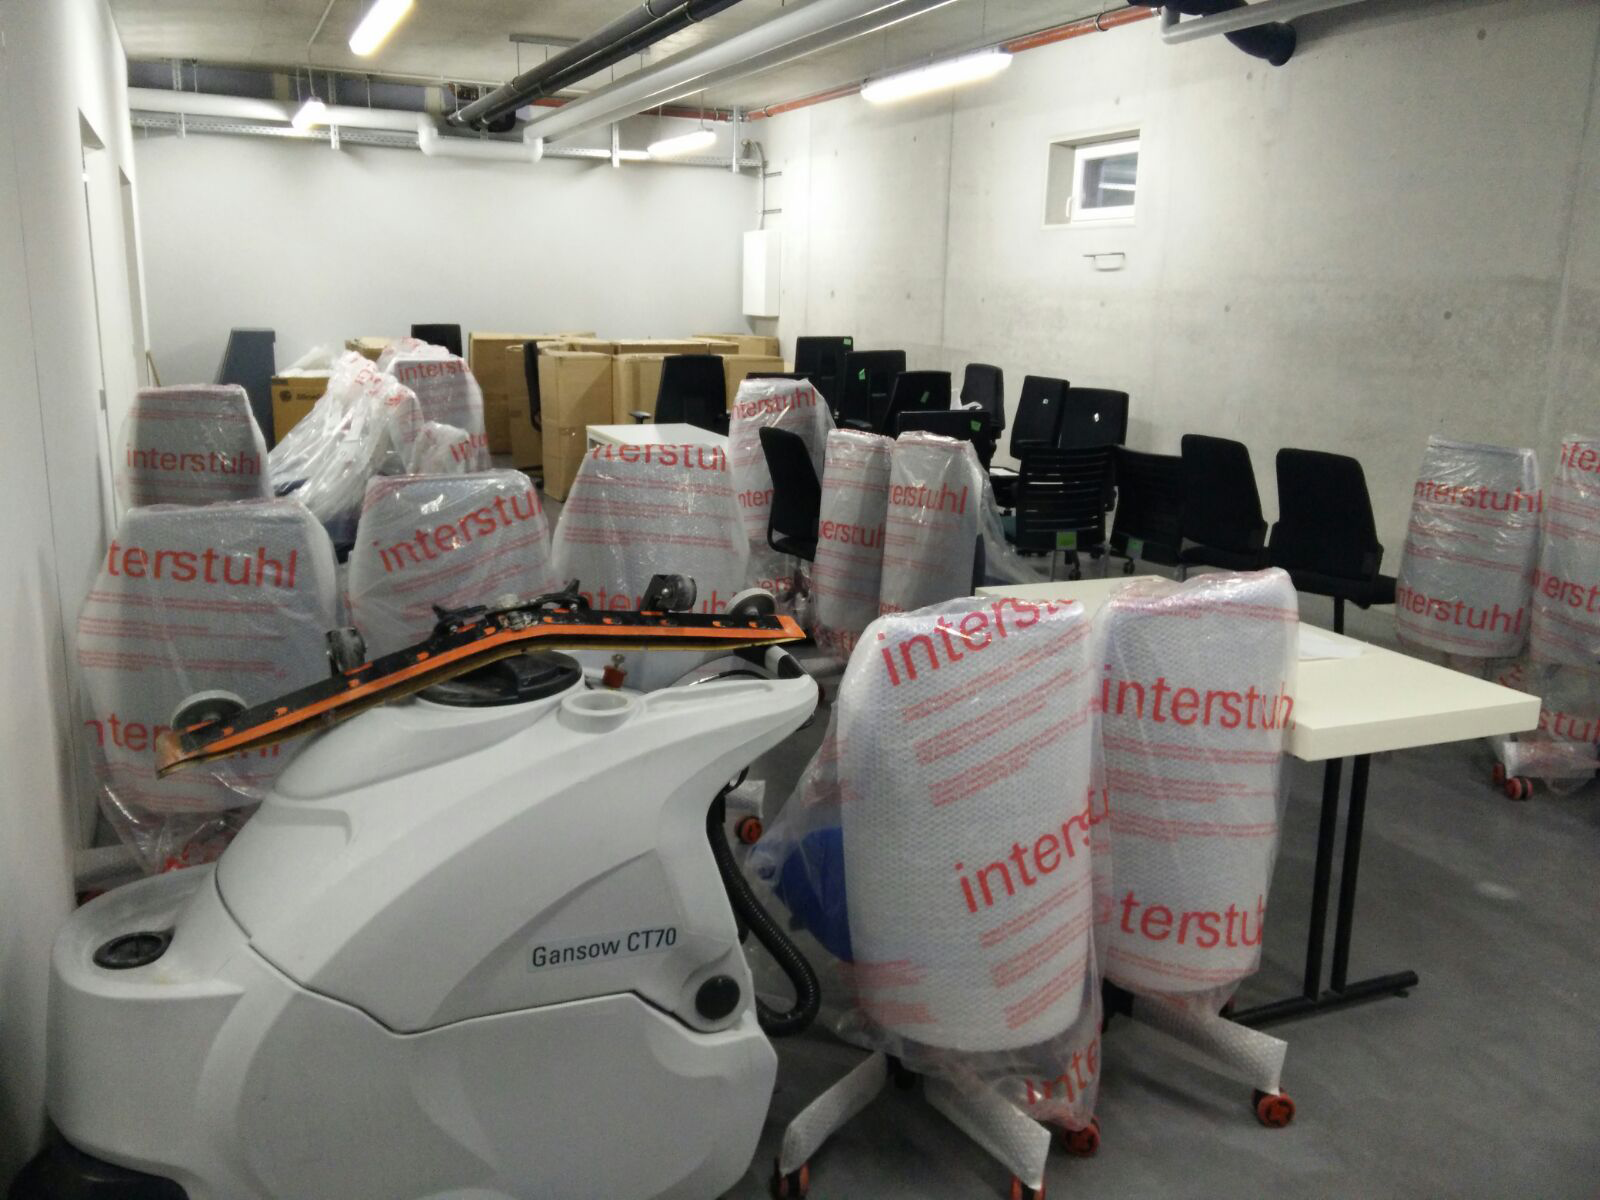
\includegraphics[width=\textwidth]{Study/study1_2_Close_Left.png}}
		\caption{Linke Seite des Labyrinths}
		\label{fig:study1_lab2}
	\end{subfigure}
	~
	\begin{subfigure}[t]{0.3\textwidth}
		\centering
		\ifthenelse{\boolean{jpg}}{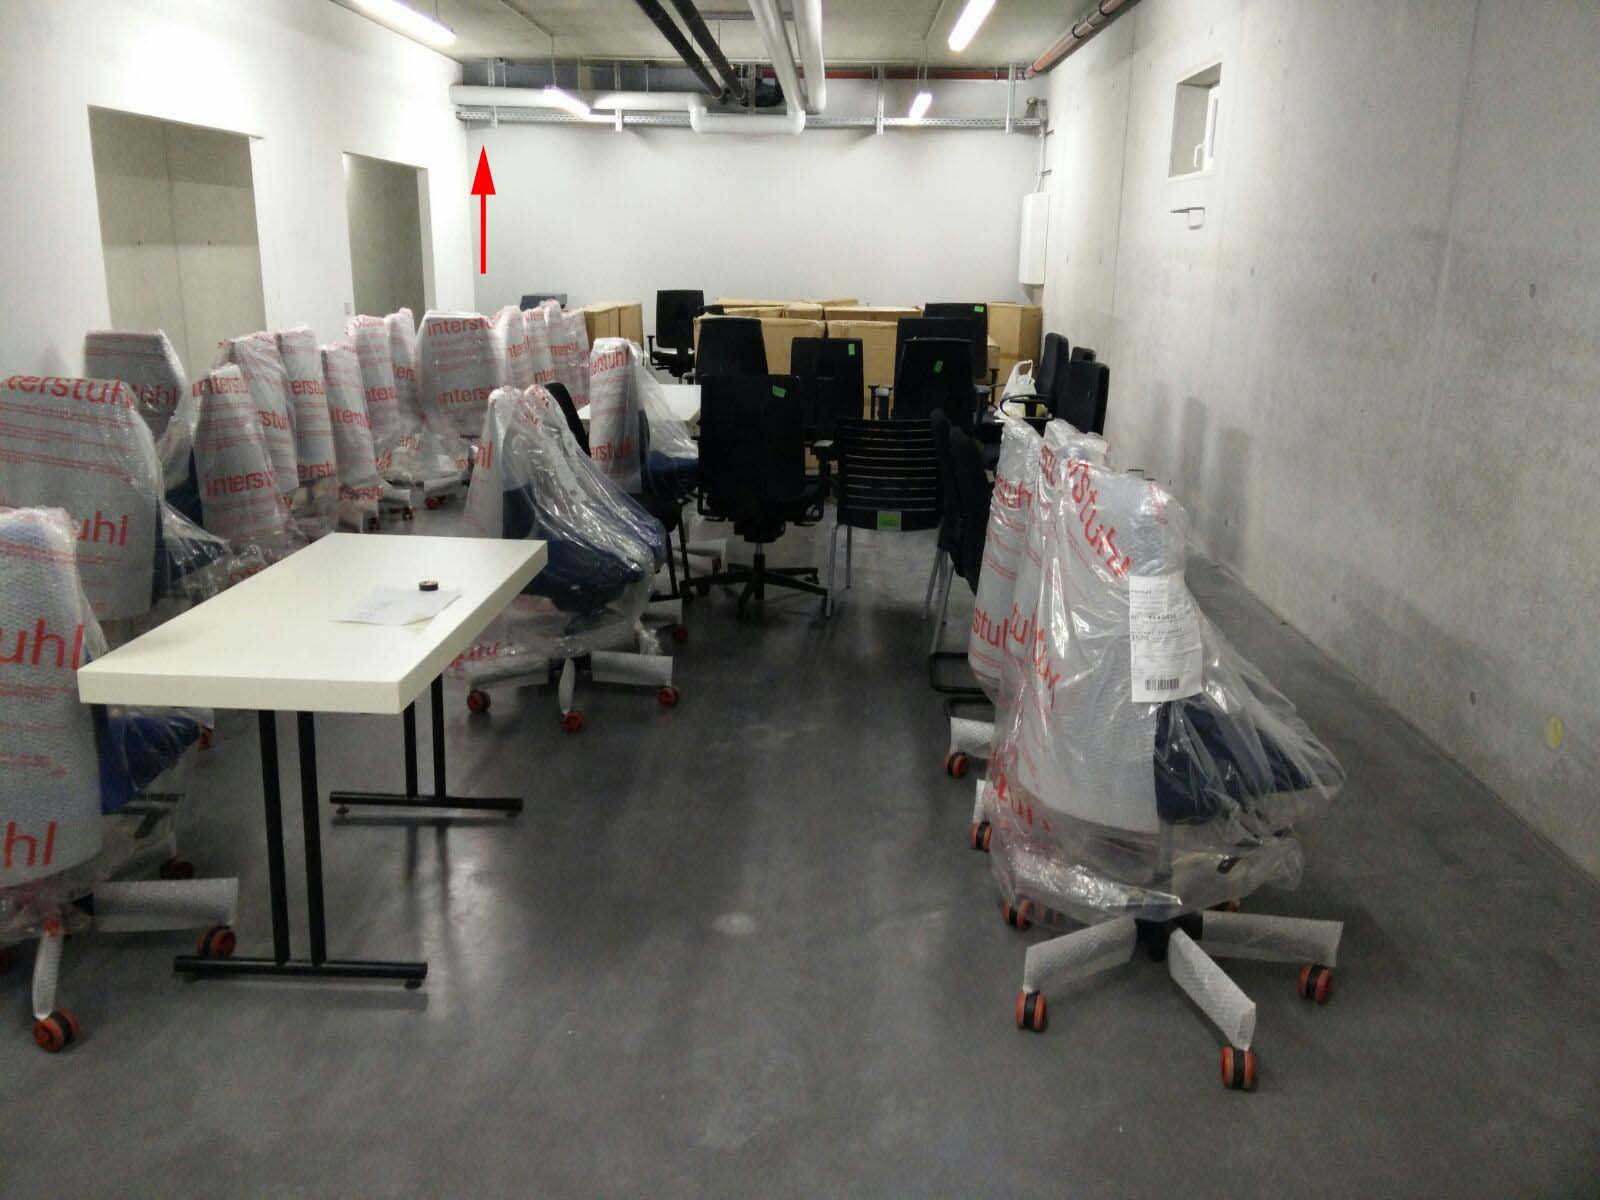
\includegraphics[width=\textwidth]{Study/study1_3_Left.jpg}}{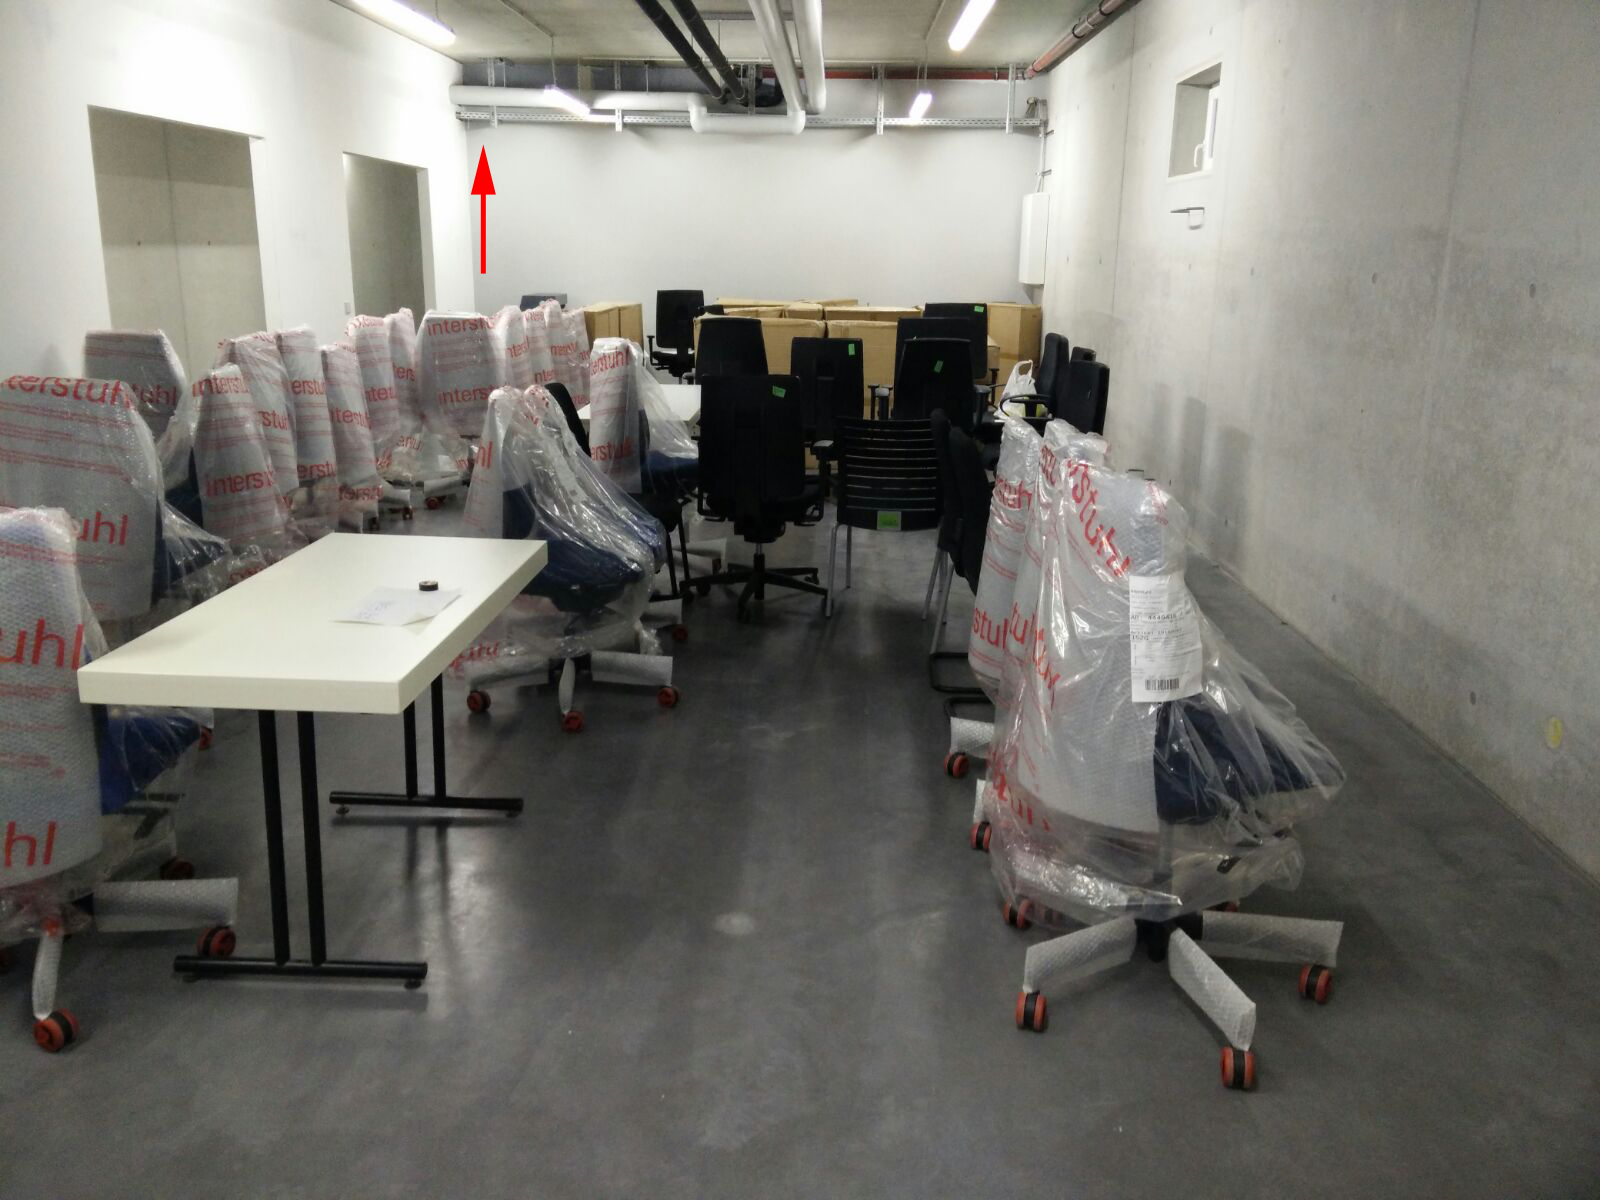
\includegraphics[width=\textwidth]{Study/study1_3_Left.png}}
		\caption{Linke Seite des Labyrinths mit Kameraposition}
		\label{fig:study1_lab3}
	\end{subfigure}
	~
	\begin{subfigure}[t]{0.3\textwidth}
		\centering
		\ifthenelse{\boolean{jpg}}{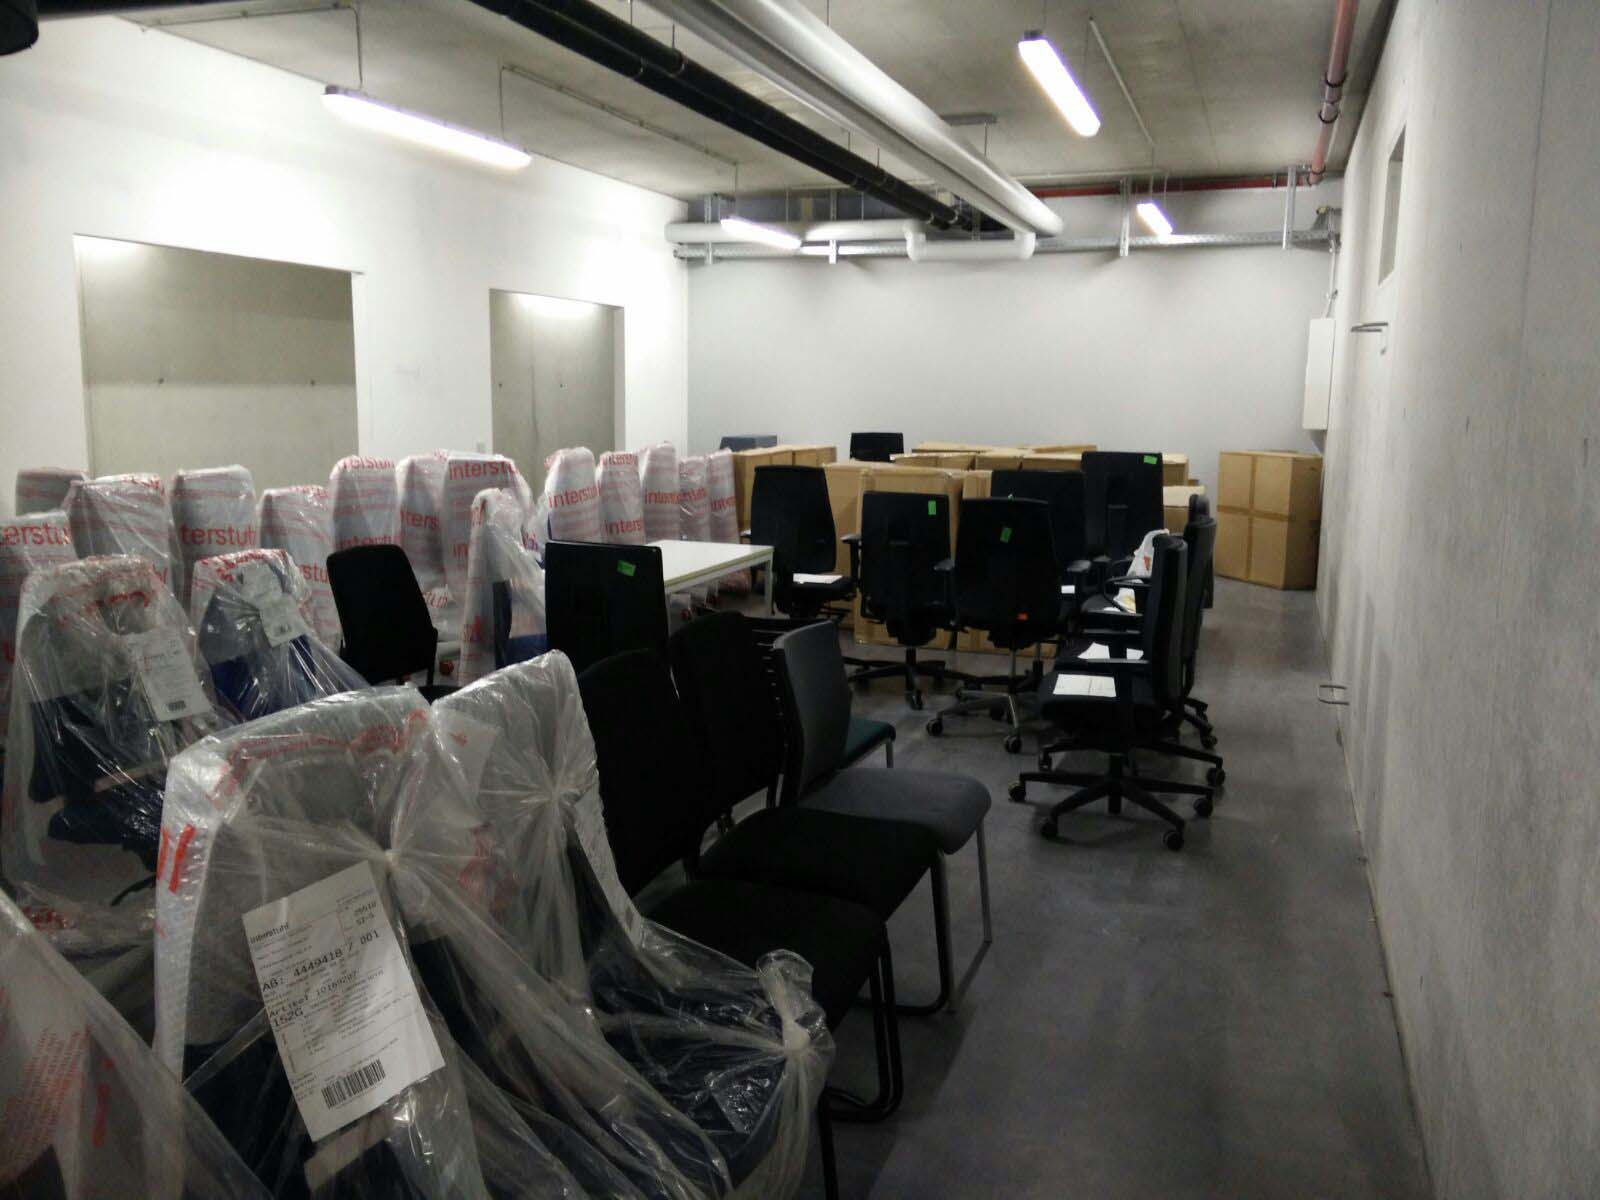
\includegraphics[width=\textwidth]{Study/study1_4_Back_Left.jpg}}{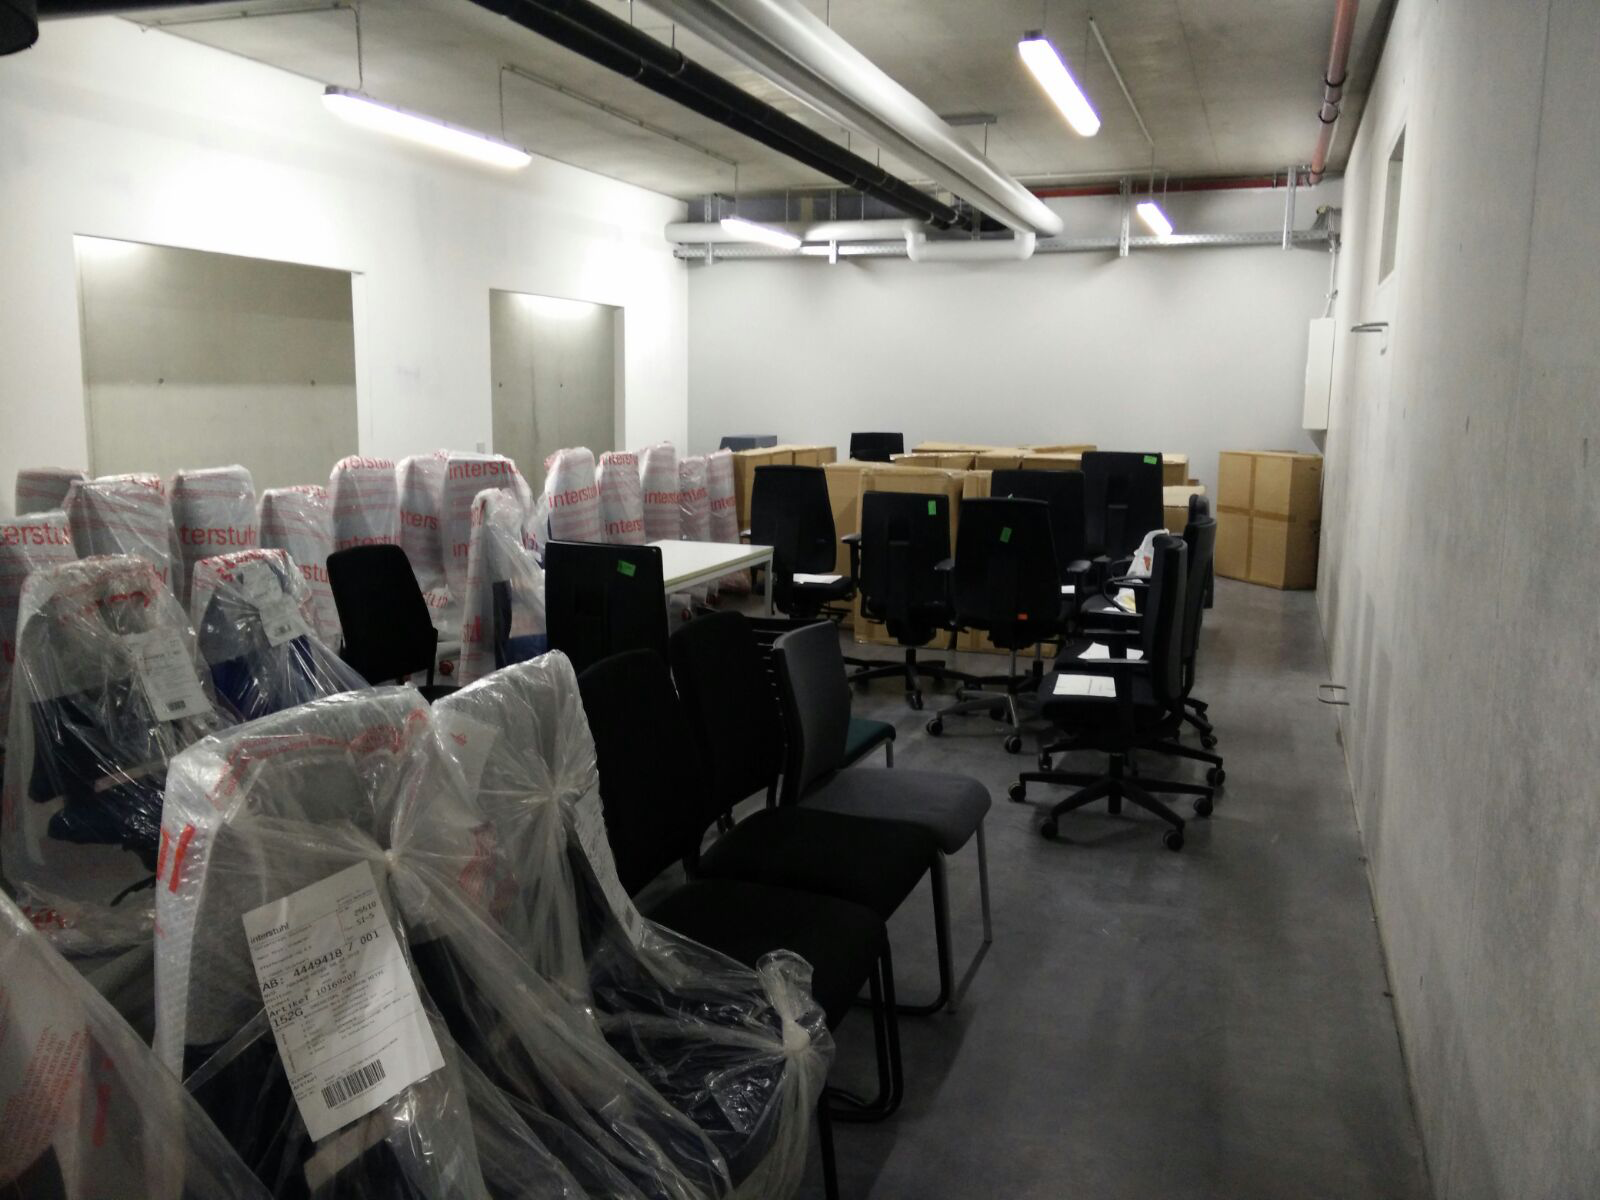
\includegraphics[width=\textwidth]{Study/study1_4_Back_Left.png}}
		\caption{Linke hintere Seite des Labyrinths}
		\label{fig:study1_lab4}
	\end{subfigure}
	~
	\begin{subfigure}[t]{0.3\textwidth}
		\centering
		\ifthenelse{\boolean{jpg}}{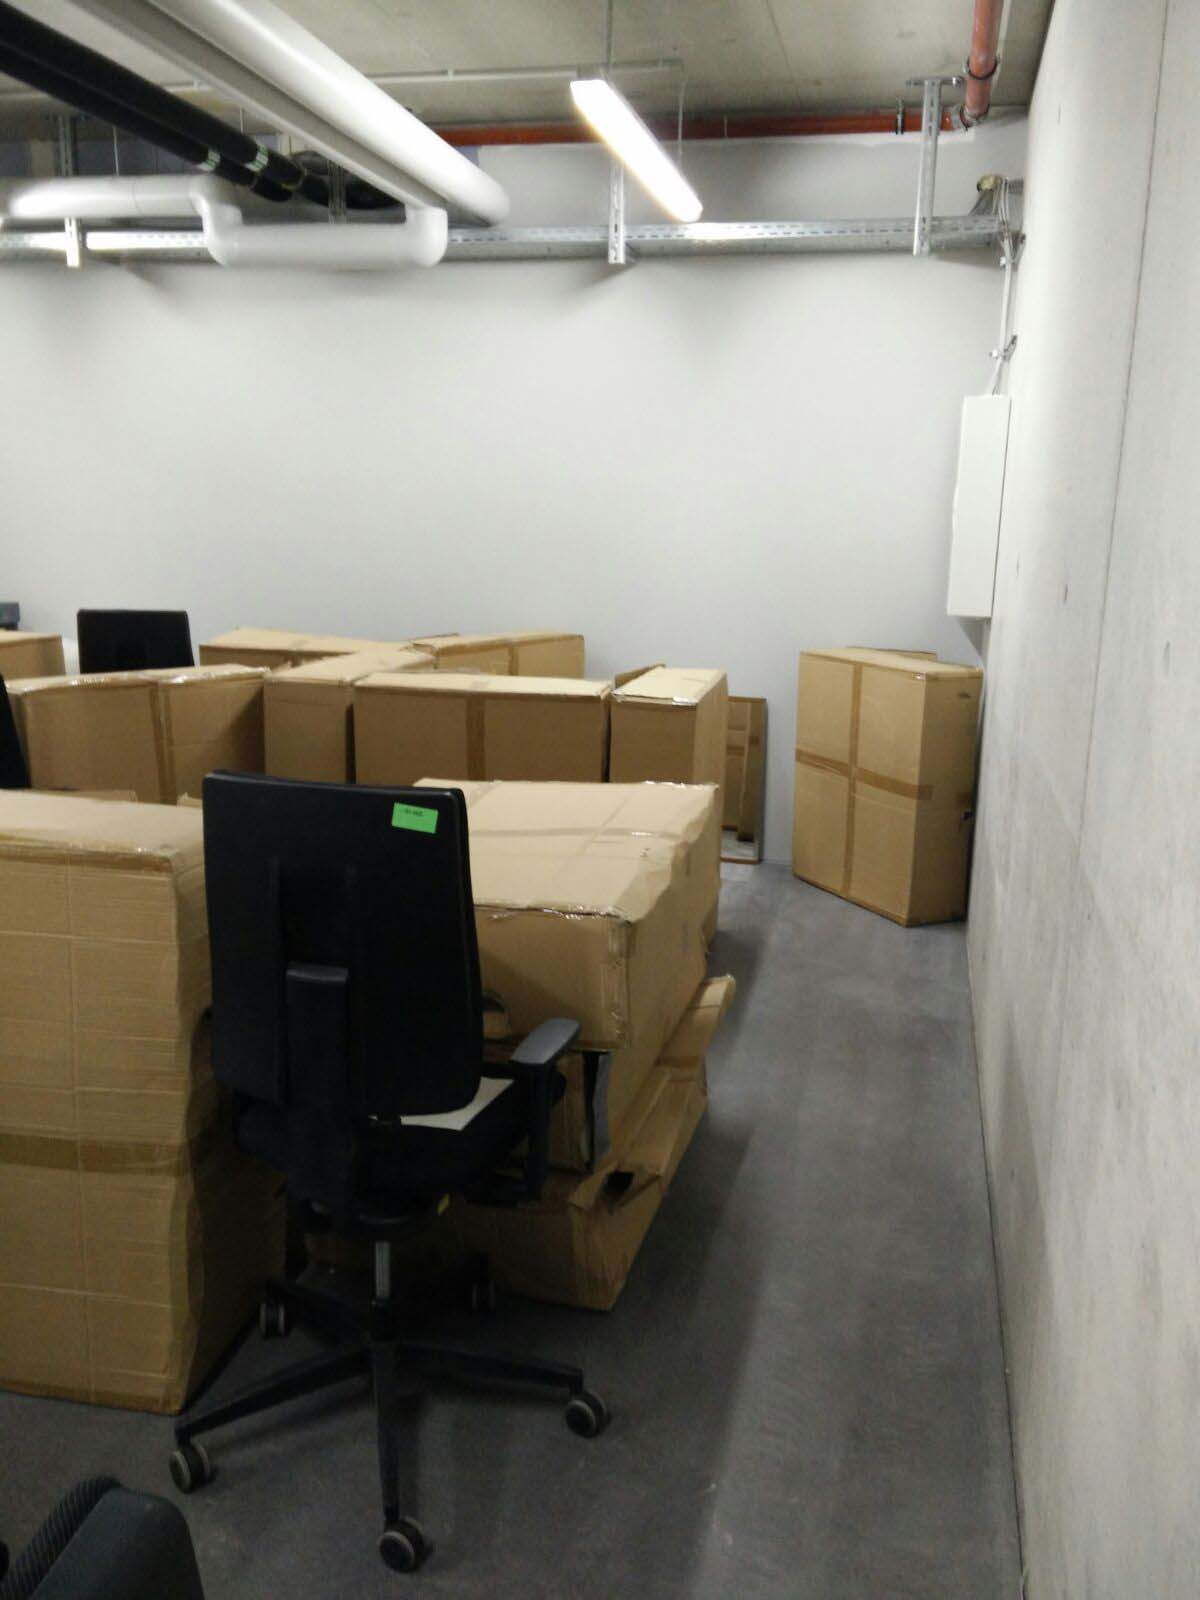
\includegraphics[width=\textwidth]{Study/study1_5_Back_Left.jpg}}{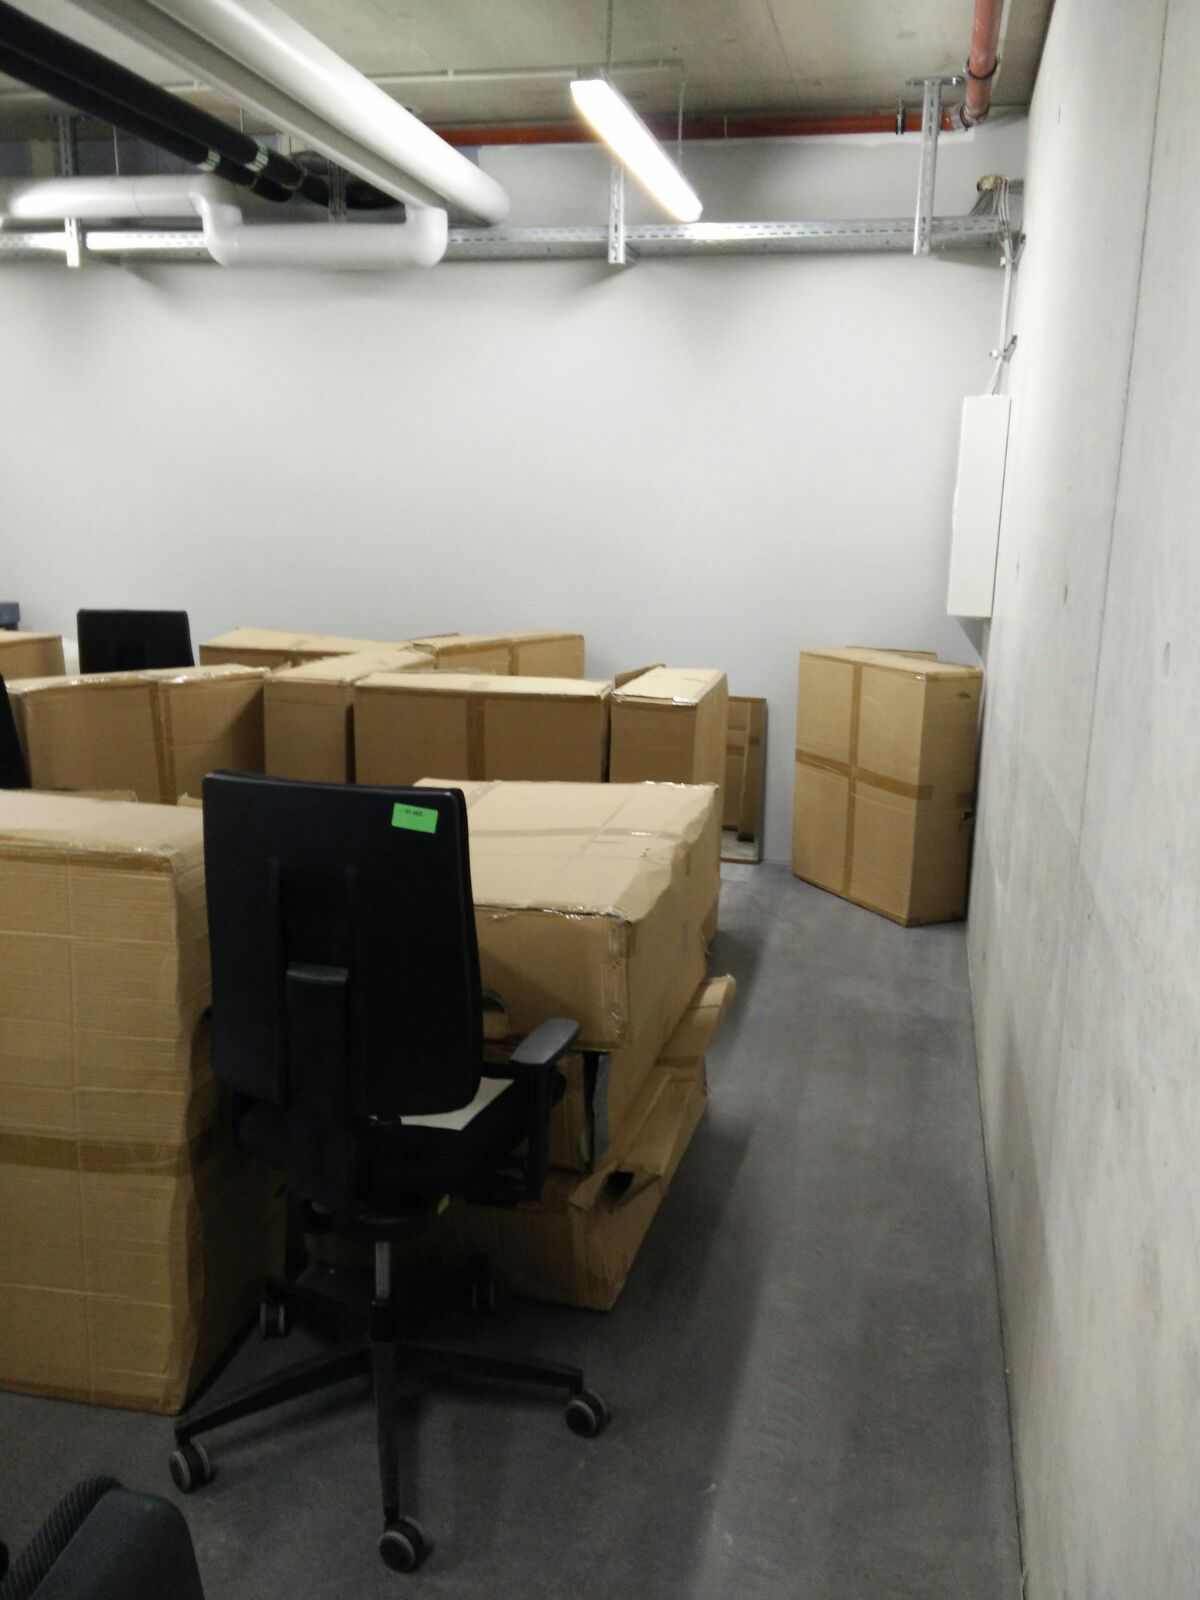
\includegraphics[width=\textwidth]{Study/study1_5_Back_Left.png}}
		\caption{Linke hintere Seite des Labyrinths}
		\label{fig:study1_lab5}
	\end{subfigure}
	~
	\begin{subfigure}[t]{0.3\textwidth}
		\centering
		\ifthenelse{\boolean{jpg}}{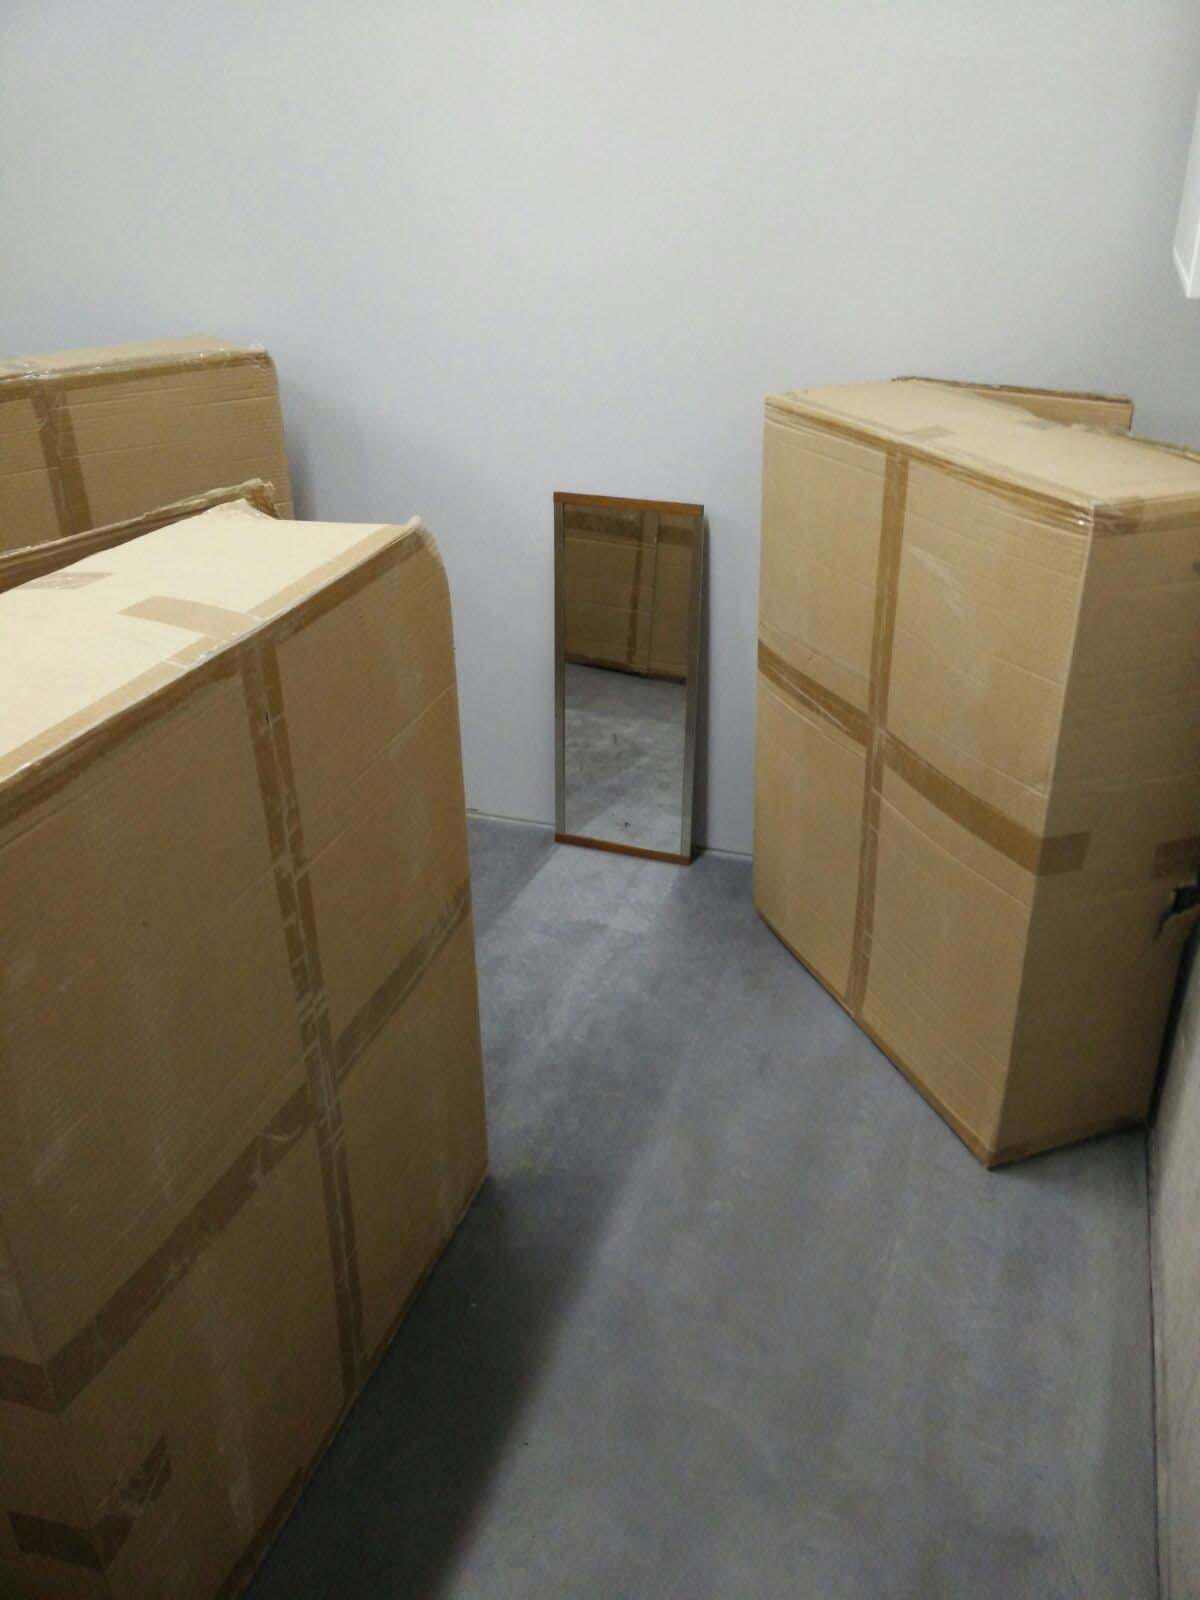
\includegraphics[width=\textwidth]{Study/study1_6_Back_Left_Corner.jpg}}{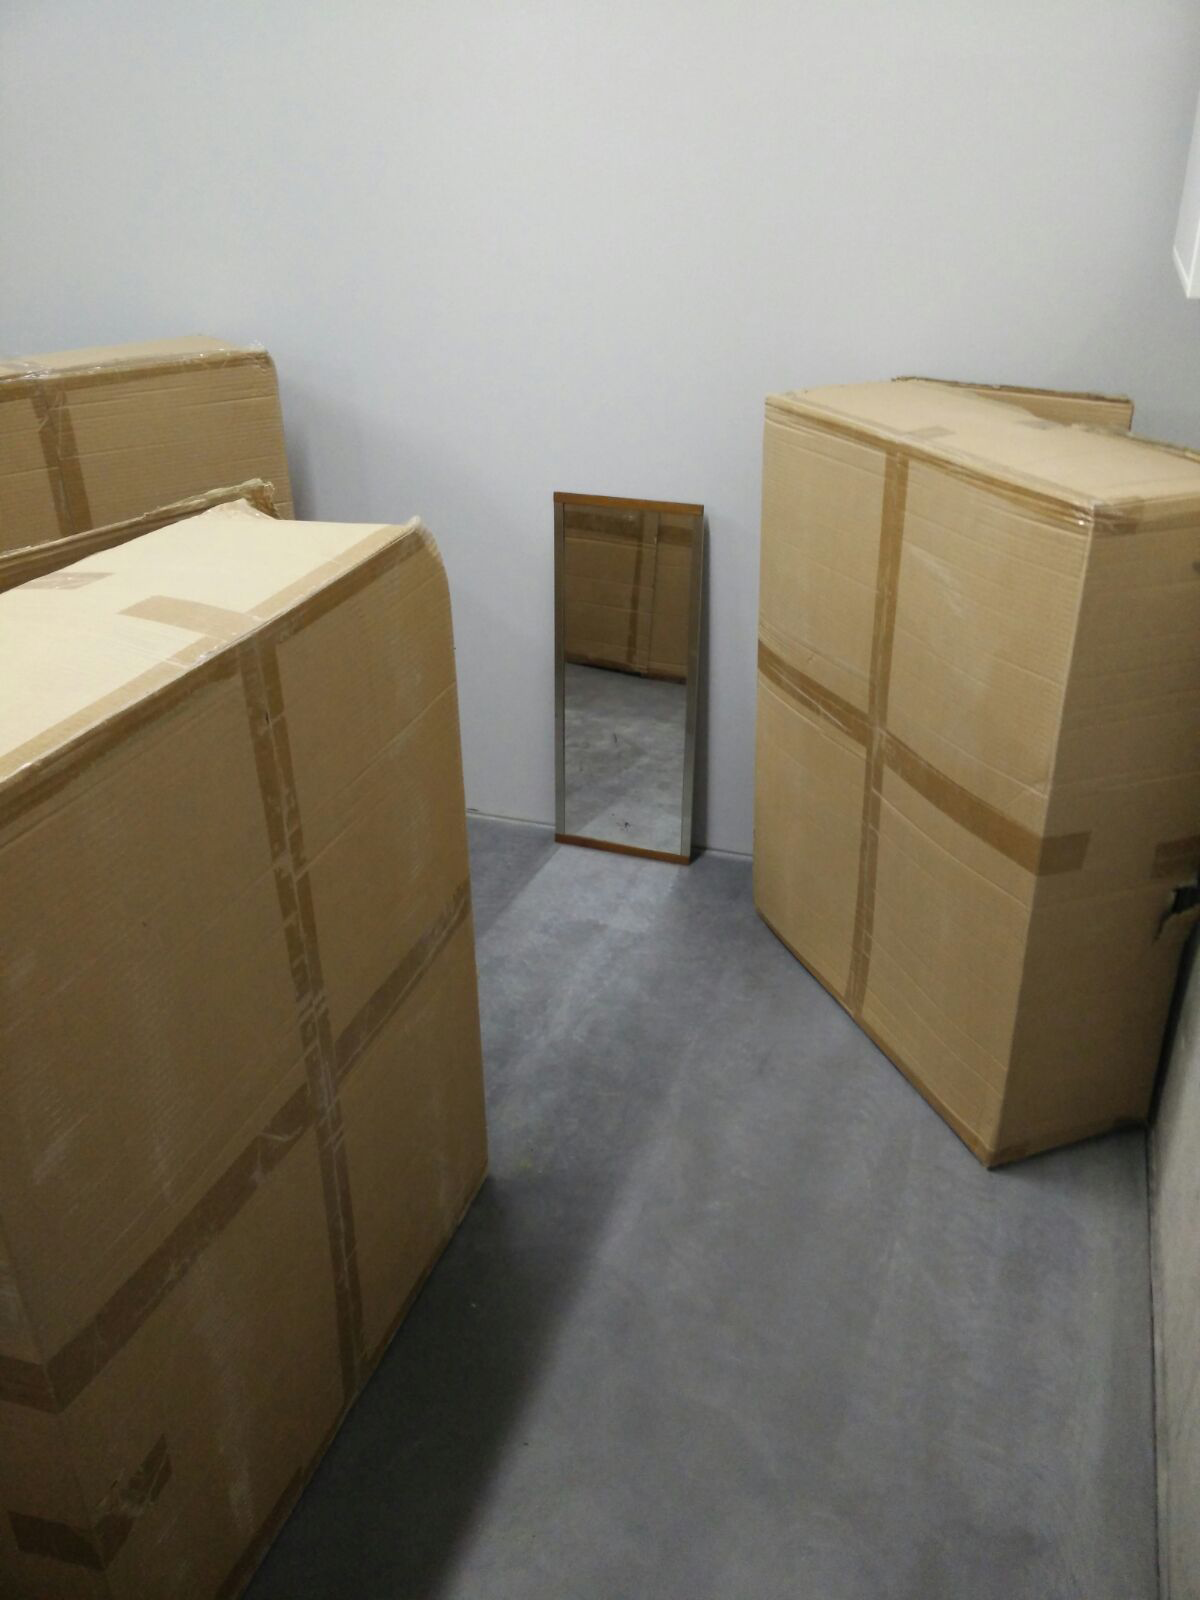
\includegraphics[width=\textwidth]{Study/study1_6_Back_Left_Corner.png}}
		\caption{Linke hintere Ecke des Labyrinths}
		\label{fig:study1_lab6}
	\end{subfigure}
	~
	\begin{subfigure}[t]{0.3\textwidth}
		\centering
		\ifthenelse{\boolean{jpg}}{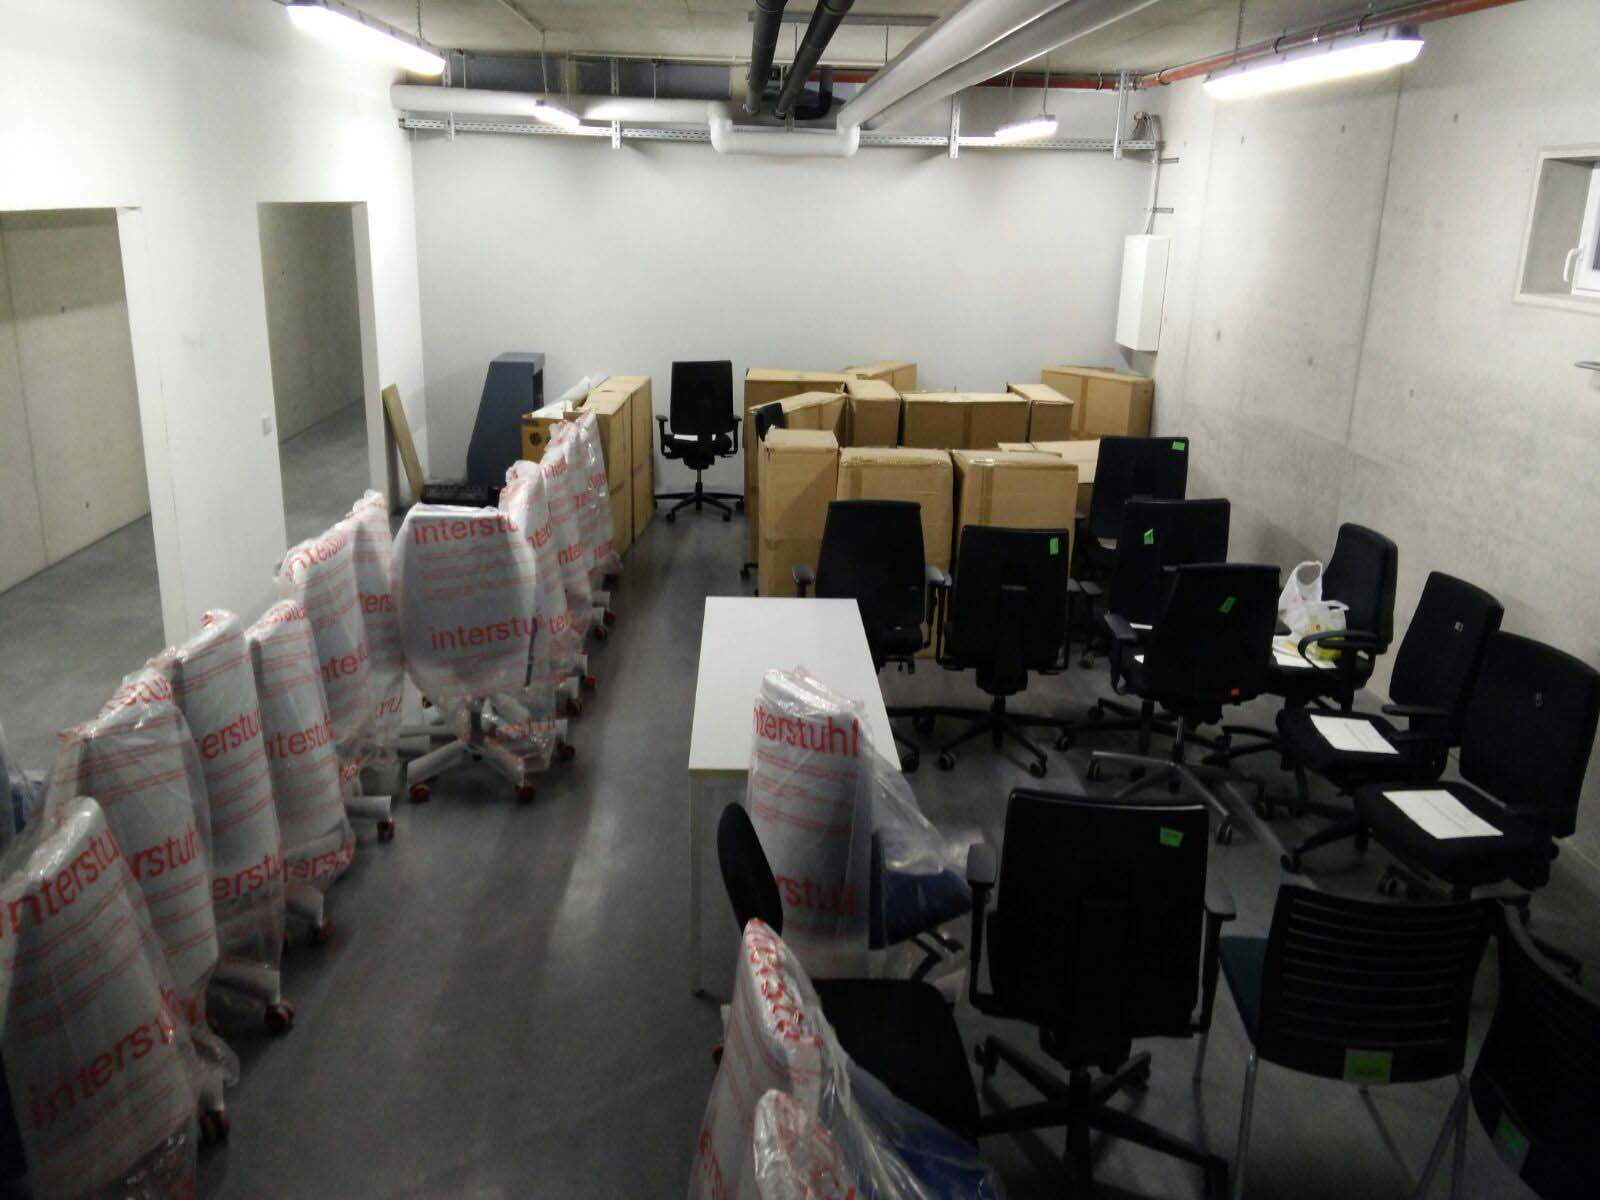
\includegraphics[width=\textwidth]{Study/study1_7_Overview_Left.jpg}}{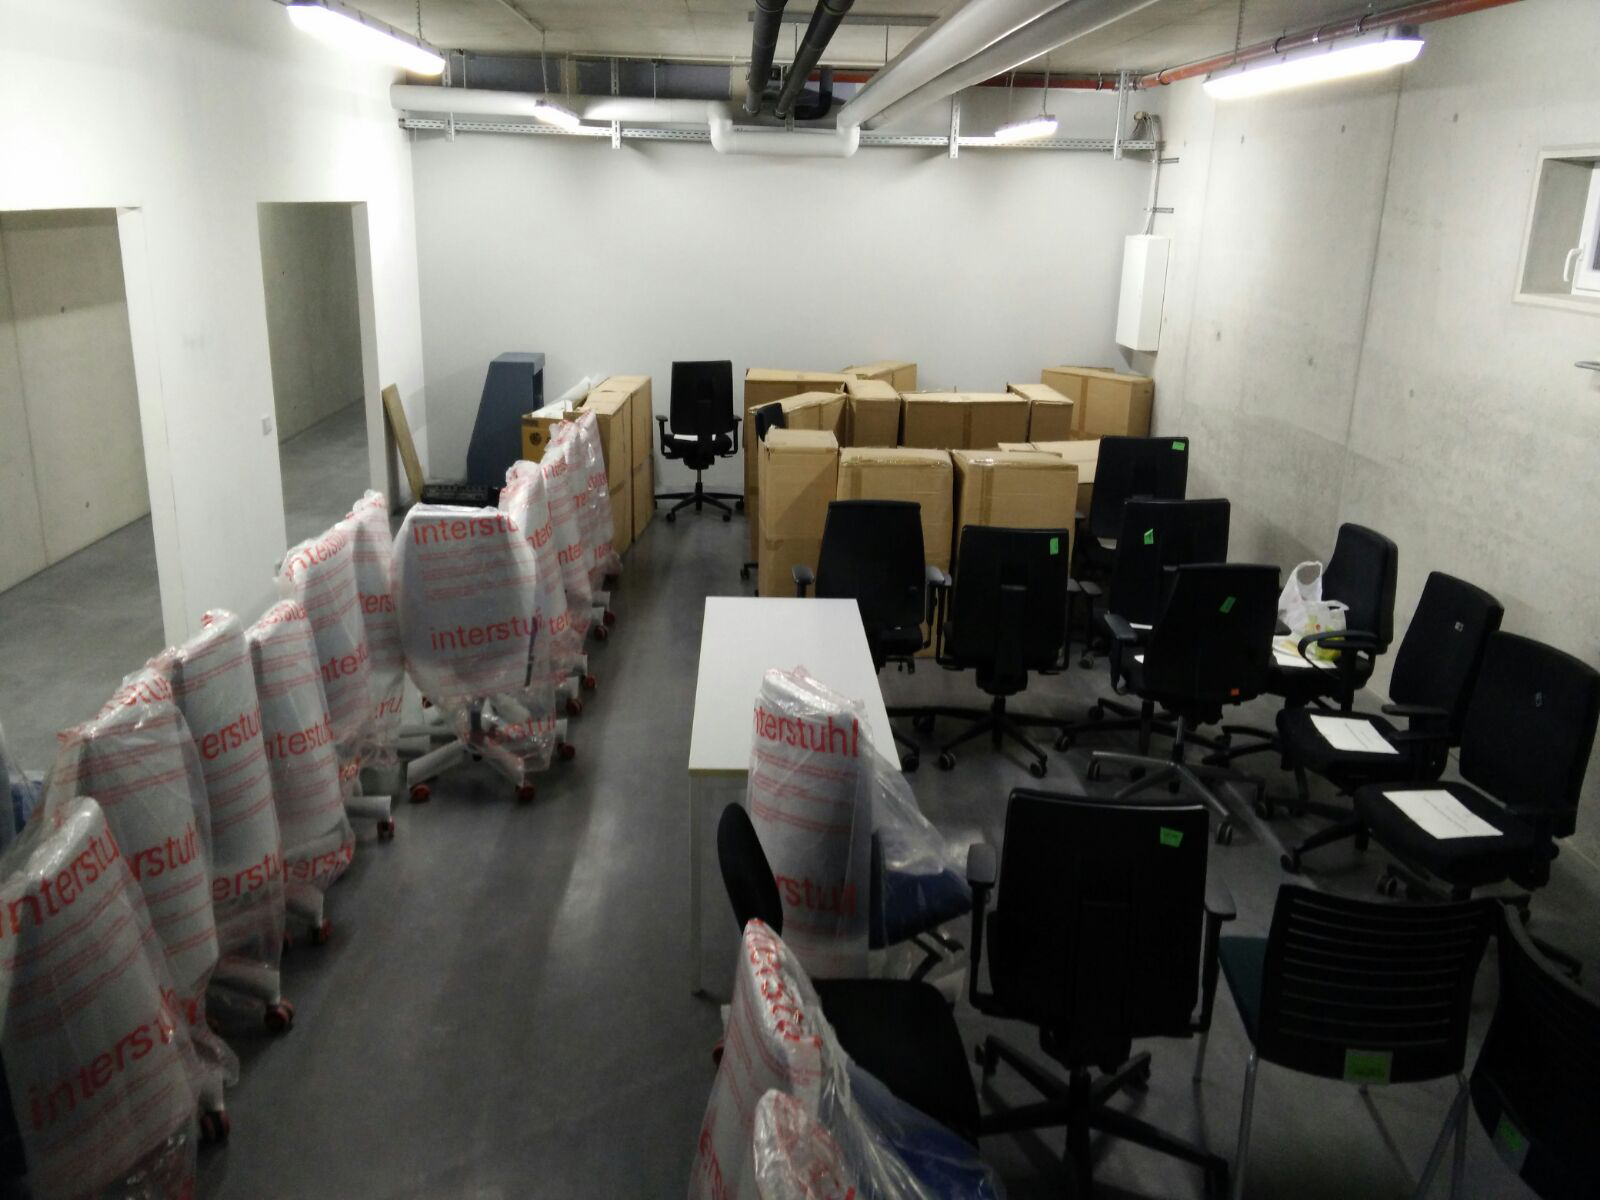
\includegraphics[width=\textwidth]{Study/study1_7_Overview_Left.png}}
		\caption{Übersicht der linken Seite des Labyrinths}
		\label{fig:study1_lab7}
	\end{subfigure}
	~
	\begin{subfigure}[t]{0.3\textwidth}
		\centering
		\ifthenelse{\boolean{jpg}}{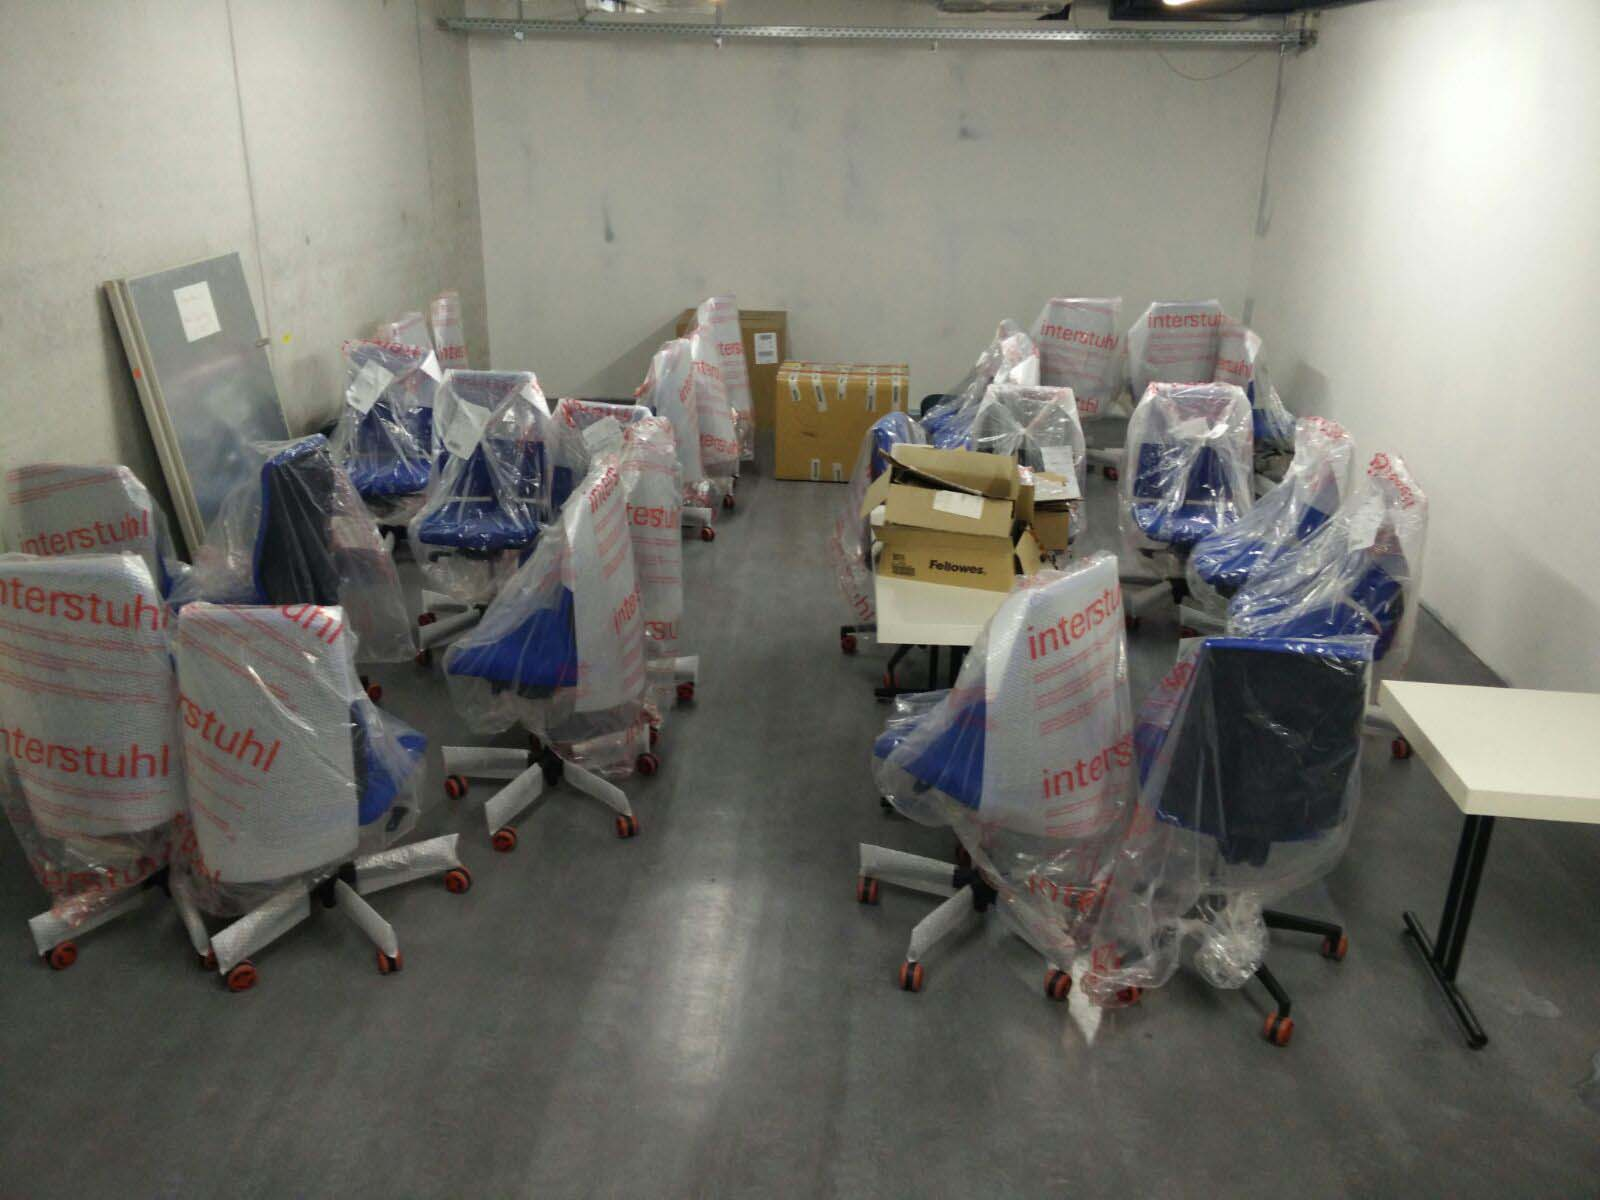
\includegraphics[width=\textwidth]{Study/study1_8_Right.jpg}}{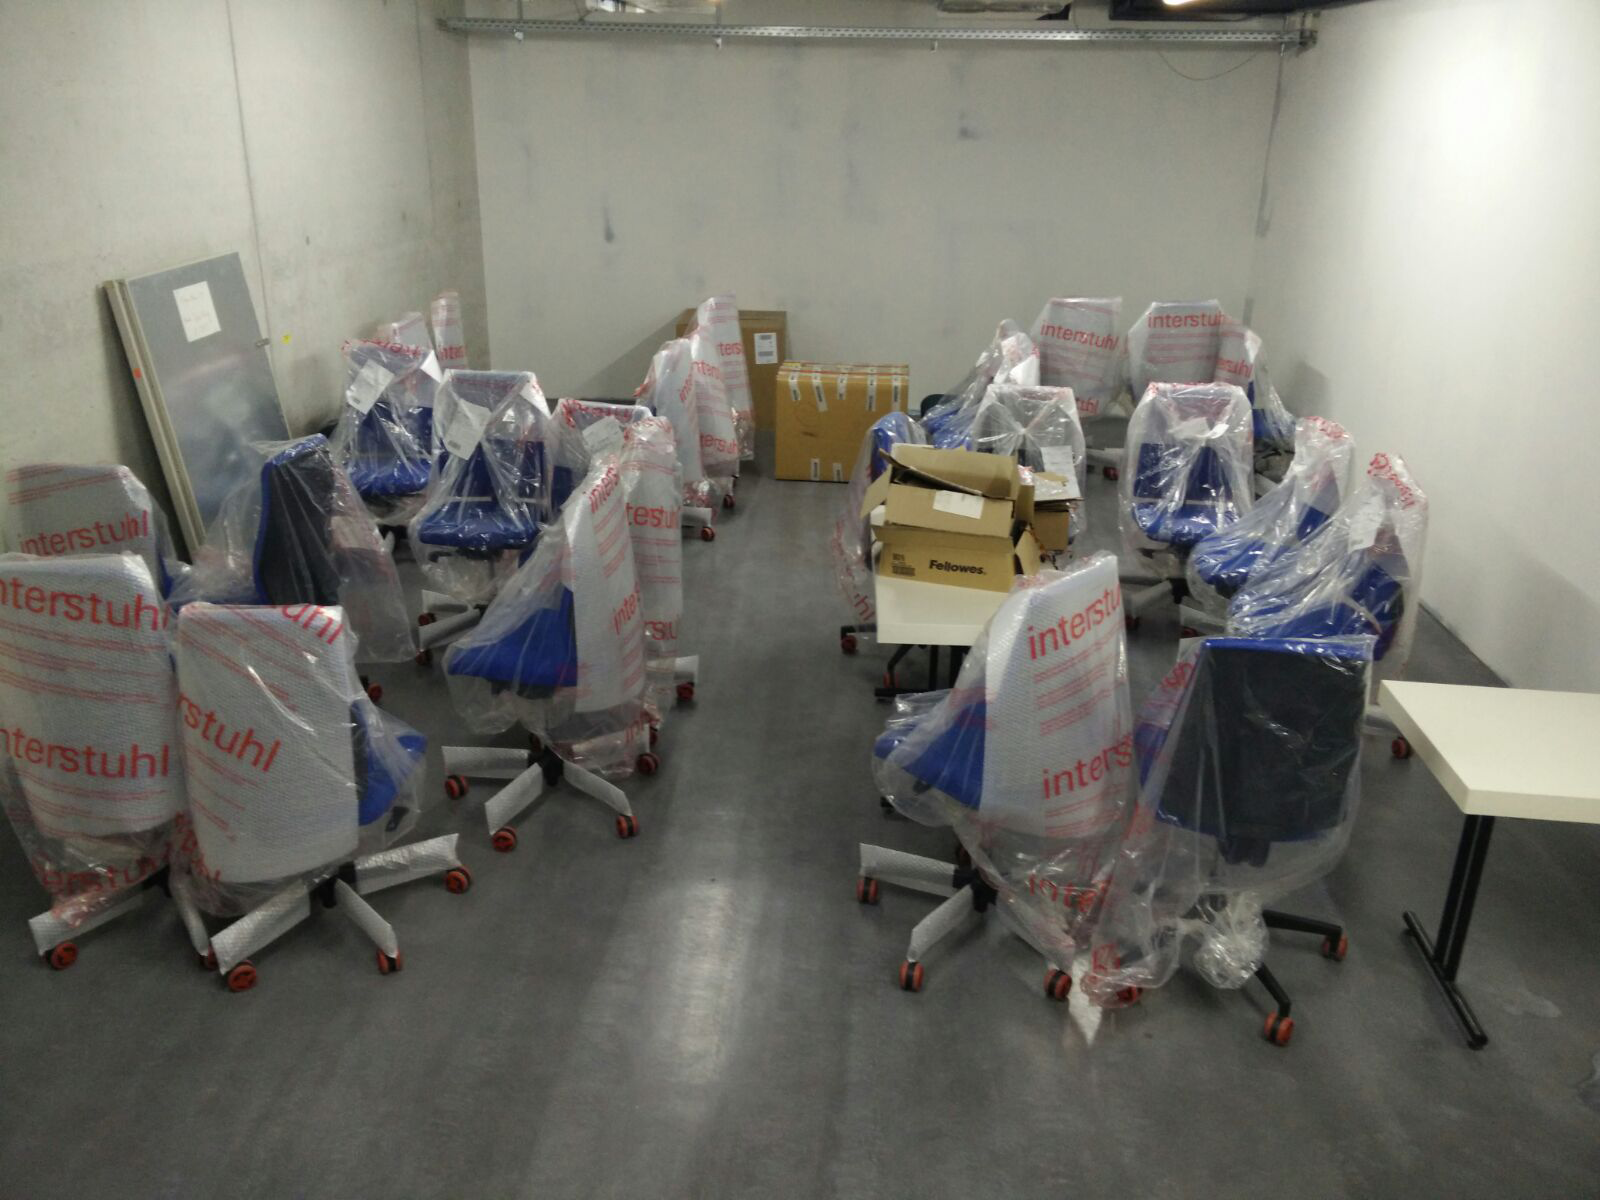
\includegraphics[width=\textwidth]{Study/study1_8_Right.png}}
		\caption{Übersicht der rechten Seite des Labyrinths}
		\label{fig:study1_lab8}
	\end{subfigure}
	~
	\begin{subfigure}[t]{0.3\textwidth}
		\centering
		\ifthenelse{\boolean{jpg}}{\includegraphics[width=\textwidth]{Study/study1_9_Middle_Right.jpg}}{\includegraphics[width=\textwidth]{Study/study1_9_Middle_Right.png}}
		\caption{Rechte Seite des Labyrinths mit Kameraposition}
		\label{fig:study1_lab9}
	\end{subfigure}
	\caption{Bilder des Aufbaus der ersten Studie}
	\label{fig:study1_lab}
\end{figure}

\begin{figure}[H]
	\begin{subfigure}[t]{0.45\textwidth}
		\centering
		\ifthenelse{\boolean{jpg}}{\includegraphics[width=\textwidth]{Study/study1_usability_pre.jpg}}{\includegraphics[width=\textwidth]{Study/study1_usability_pre.png}}
		
		\label{fig:study1_usa_pre}
	\end{subfigure}
	~
	\begin{subfigure}[t]{0.45\textwidth}
		\centering
		\ifthenelse{\boolean{jpg}}{\includegraphics[width=\textwidth]{Study/study1_usability_post.jpg}}{\includegraphics[width=\textwidth]{Study/study1_usability_post.png}}
		\caption{Eingestufte Bedienbarkeit nach Ende}
		\label{fig:study1_usa_post}
	\end{subfigure}
	\caption{Interview-Ergebnisse}
	\label{fig:study1_usa}
\end{figure}

\subsection{Ergebnisse}
Die durchschnittliche Studiendurchlaufsdauer lag bei 8,3 Minuten, dabei gab es allerdings, wie in \cref{fig:study1_duration} zu sehen, einige größere Ausreißer.

\cref{fig:study1_use} zeigt, dass der mögliche Nutzen des Prototypen durchweg als sehr gut eingestuft wurde.

Probanden würden den Prototypen, allerdings nicht zwingend weiterempfehlen, wie \cref{fig:study1_recom} zeigt.

Generell hatten die Probanden einen positiven Eindruck von dem Prototypen, wie \cref{fig:study1_impres} zeigt.

Die Bedienbarkeit des Prototypen lag, laut den Studienteilnehmern, von Anfang an in einem hohen Bereich und verbesserte sich, wie an \cref{fig:study1_usa} über die Studie hinweg.

Das Tiefenbild wurde in 87\% der Zeit von den Probanden genutzt.
Die durchschnittliche Abweichung der Raumschätzung von der tatsächlichen Größe betrug 0,75m in der Länge und 1m in der Breite.
Die größte Abweichung betrug 2m in Länge wie Breite.

\begin{figure}[H]
	\centering
	\begin{subfigure}[t]{0.45\textwidth}
		\centering
		\ifthenelse{\boolean{jpg}}{\includegraphics[scale=0.7]{Study/study1_duration.jpg}}{\includegraphics[scale=0.7]{Study/study1_duration.png}}
		\caption{Studiendauer}
		\label{fig:study1_duration}
	\end{subfigure}
	~
	\begin{subfigure}[t]{0.45\textwidth}
		\centering
		\ifthenelse{\boolean{jpg}}{\includegraphics[width=\textwidth]{Study/study1_use.jpg}}{\includegraphics[width=\textwidth]{Study/study1_use.png}}
		\caption{Eingestufte Nützlichkeit}
		\label{fig:study1_use}
	\end{subfigure}
	~
	\begin{subfigure}[t]{0.45\textwidth}
		\centering
		\ifthenelse{\boolean{jpg}}{\includegraphics[width=\textwidth]{Study/study1_recommendation.jpg}}{\includegraphics[width=\textwidth]{Study/study1_recommendation.png}}
		\caption{Wahrscheinlichkeit der Weiterempfehlung}
		\label{fig:study1_recom}
	\end{subfigure}
	~
	\begin{subfigure}[t]{0.45\textwidth}
		\centering
		\ifthenelse{\boolean{jpg}}{\includegraphics[width=\textwidth]{Study/study1_impression.jpg}}{\includegraphics[width=\textwidth]{Study/study1_impression.png}}
		\caption{Eindruck}
		\label{fig:study1_impres}
	\end{subfigure}
	\caption{Interview-Ergebnisse}
	\label{fig:study1_results1}
\end{figure}

\subsection{Diskussion}
Die Unterschiede in der benötigten Dauer können über unterschiedliche Strategien der Probanden erklärt werden.
Die Studienteilnehmer, welche sich zuerst einen Überblick verschafften indem sie nach der ersten Wärmequelle suchten, kamen schneller an die Wärmeflasche, als diejenigen, die sich \enquote{zufällig} für eine Richtung entschieden.
Es hat sich gezeigt, dass die Probanden hauptsächlich das Tiefenbild für die Navigation benutzten und lediglich an Abzweigungen oder anderen strategischen Punkten auf das Wärmebild wechselten, um zu überprüfen, ob sich ein warmer Gegenstand im Blickfeld befindet.

Auch zeigt die relativ geringe Abweichung, bei der Raumschätzung, dass der Prototyp die räumliche Wahrnehmung und das Gefühl für Distanzen stärkt.

Die etwas geringe Wahrscheinlichkeit für eine Weiterempfehlung des Prototyps, trotz der anderweitig hohen Einstufung, wurde von den Teilnehmern damit begründet, dass dieser Prototyp für spezielle Situationen gedacht ist, welche nicht häufig im alltägliche Leben vorkommen.

Die Probanden wünschten sich in den Interviews ein fusioniertes Bild, da sie das häufige Wechseln als störend empfanden.
Diejenigen, die genauer darauf eingingen, beschrieben ihre Vorstellung davon ähnlich \nameref{sec:fusion_post-render}.

Einige wünschten sich ein anderes Farbspektrum für die Wärmebildkamera, da sie, mit dem häufigem Wechseln, die Bildmodi teilweise verwechselten.

Wenige Studienteilnehmer empfanden den weißen Balken mit den Bildmittelpunktinformationen als störend und hätten diesen lieber durch ein Kästchen im Bild ersetzt.
Andere hätten auf diesem Balken noch gerne eine Legende gesehen.

Im ganzen, kann diese erste Stufe des Prototypen als Erfolg gewertet werden.
Es folgt nun die Verbesserung des Prototypen und eine ähnliche Studie mit Probanden, welche Erfahrungen mit Wärmebildkameras gesammelt haben.

\section{Studie 2}

\subsection{Methode}
Die Probanden wurden in einen komplett abgedunkelten Raum geführt und mussten zuerst die Deckenhöhe schätzen.
Darauf sollten sie durch den Raum zu einem anderen Ausgang navigieren und dabei den wärmsten Punkt im Raum entdecken.
Der unterstützende Prototyp, den die Probanden erhielten, bestand aus einer tragbaren Halterung für eine Wärme- und Tiefenbildkamera, mit angebrachtem Handy als Anzeigemöglichkeit oder einem Feuerwehrhelm, an welchem diese Halterung montiert war, mit einer Augmented Reality Brille.
Nutzer hatten Wärme- oder Tiefenbild oder die erstellte Fusion aus Beidem zur Verfügung.

\subsection{Design}
Jeder Proband wurde nur einmal in den Raum geführt.
Dabei wurden die Probanden in zwei Teilgruppen aufgesplittet.
Die eine erhielt den Handheld Prototypen, die andere die Helmhalterung mit Brille.
Es gab keine Einschränkung in der Auswahl der Bildmodi.
Auch ihre Bewegungen wurden nicht eingeschränkt oder in eine Richtung geleitet.

\subsubsection{Probanden}
Zur Studiendurchführung wurden 11 Probanden zwischen 19 und 51 Jahren befragt.
Aus dieser Gruppe hat noch niemand bisherige Erfahrungen mit Tiefenbildkameras gesammelt.
Die Probanden kamen dabei aus unterschiedlichen Berufsfeldern, wobei alle Mitglieder einer freiwilligen Feuerwehr waren.
Alle hatten bereits einige Erfahrung mit Wärmebildkameras.
Es gab nur eine weibliche Studienteilnehmerin.

Dabei wurden sechs Probanden mit dem Headmounted-Prototypen und die anderen fünf mit dem Handheld-Prototypen ausgestattet.

\subsection{Vorgehen}

\subsubsection{Die Aufgabe}
Die Probanden wurden empfangen, über ihre Rechte und den Zweck des Prototypen sowie der Studie aufgeklärt und in die Funktionsweise des Prototypen eingewiesen.
Darauf wurden sie in einen bereits zuvor abgedunkelten Raum geführt.
Dies hat den Grund, die visuelle Wahrnehmung des Probanden möglichst stark einzuschränken und eine \enquote{normale} Navigation zu verhindern.
Damit ist der Prototyp die einzige visuelle Hilfe, auf die sich der Proband verlassen kann.
\cref{fig:study2_proto_hand} stellt den Handheld-Prototyp dar, \cref{fig:study2_proto_head} den am Helm befestigten.
Es standen der Wärme- und Tiefenbildmodus, sowie die erstellte Fusion aus beiden als Hilfe zur Verfügung.
Entfernung und Temperatur des am Bildmittelpunkt gemessenen Wertes wurde auch angezeigt.
Bilder des Wärmebilds, Tiefenbilds und der Fusion sind in \cref{fig:study2_mode} enthalten.

Die Probanden wurden zuerst in den abgedunkelten Raum geleitet.
Dort sollten sie die Deckenhöhe messen und dann zu einem Ausgang auf der anderen Seite des Raums navigieren.
Während dieser Zeit sollten sie zudem die heißeste Temperatur ausfindig machen.
\cref{fig:study2_room} zeigt den Raum und die darin platzierten Hindernisse, \cref{fig:study2_study} zeigt zudem weitere Bilder der Studie.

\begin{figure}[H]
	\begin{subfigure}[t]{0.3\textwidth}
		\centering
		\ifthenelse{\boolean{jpg}}{\includegraphics[width=\textwidth]{Study/study2_fus.jpg}}{\includegraphics[width=\textwidth]{Study/study2_fus.png}}
		\caption{Fusionsmodus}
		\label{fig:study2_fus0}
	\end{subfigure}
	~
	\begin{subfigure}[t]{0.3\textwidth}
		\centering
		\ifthenelse{\boolean{jpg}}{\includegraphics[width=\textwidth]{Study/study2_depth.jpg}}{\includegraphics[width=\textwidth]{Study/study2_depth.png}}
		\caption{Tiefenbild}
		\label{fig:study2_depth}
	\end{subfigure}
	~
	\begin{subfigure}[t]{0.3\textwidth}
		\centering
		\ifthenelse{\boolean{jpg}}{\includegraphics[width=\textwidth]{Study/study2_ir.jpg}}{\includegraphics[width=\textwidth]{Study/study2_ir.png}}
		\caption{Wärmebild}
		\label{fig:study2_ir}
	\end{subfigure}
	\caption{Bildmodi}
	\label{fig:study2_mode}
\end{figure}

Dabei wurde sowohl die benötigte Dauer, sowie wie lange welcher Modus genutzt wurde gemessen.
Zusätzlich wurde die Ausgabe aufgenommen.
Der ganze Verlauf wurde von einer Infrarotkamera aufgezeichnet und gleichzeitig darüber überwacht.
Die Zeit, die der Proband zum Lösen der Aufgaben hatte, betrug zehn Minuten.

\begin{figure}[H]
	\centering
	\begin{subfigure}[t]{0.55\textwidth}
		\centering
		\ifthenelse{\boolean{jpg}}{\includegraphics[width=\textwidth]{Study/study2_proto_hand_model.jpg}}{\includegraphics[width=\textwidth]{Study/study2_proto_hand_model.png}}
		\caption{Schematischer Aufbau des Handheld-Prototyps}
		\label{fig:study2_proto_hand_model}
	\end{subfigure}
	~
	\begin{subfigure}[t]{0.4\textwidth}
		\centering
		\ifthenelse{\boolean{jpg}}{\includegraphics[width=\textwidth]{Study/study2_proto_halterung.jpg}}{\includegraphics[width=\textwidth]{Study/study2_proto_halterung.png}}
		\caption{3D-Modell der Halterung}
		\label{fig:study2_proto_halterung}
	\end{subfigure}
	~
	\begin{subfigure}[t]{0.25\textwidth}
		\centering
		\ifthenelse{\boolean{jpg}}{\includegraphics[width=\textwidth]{Study/study2_proto_hand_front.jpg}}{\includegraphics[width=\textwidth]{Study/study2_proto_hand_front.png}}
		\caption{Realer Handheld-Prototyp}
		\label{fig:study2_proto_hand_front}
	\end{subfigure}
	~
	\begin{subfigure}[t]{0.25\textwidth}
		\centering
		\ifthenelse{\boolean{jpg}}{\includegraphics[width=\textwidth]{Study/study2_proto_hand_side.jpg}}{\includegraphics[width=\textwidth]{Study/study2_proto_hand_side.png}}
		\caption{Realer Handheld-Prototyp}
		\label{fig:study2_proto_hand_side}
	\end{subfigure}
	\caption{Tragbarer Prototyp + Halterung}
	\label{fig:study2_proto_hand}
\end{figure}

\begin{figure}[H]
	\centering
	\begin{subfigure}[t]{0.45\textwidth}
		\centering
		\ifthenelse{\boolean{jpg}}{\includegraphics[width=\textwidth]{Study/study2_proto_head_model.jpg}}{\includegraphics[width=\textwidth]{Study/study2_proto_head_model.png}}
		\caption{Schematischer Aufbau des Prototyps}
		\label{fig:study2_proto_head_model}
	\end{subfigure}
	~
	\begin{subfigure}[t]{0.25\textwidth}
		\centering
		\ifthenelse{\boolean{jpg}}{\includegraphics[width=\textwidth]{Study/study2_proto_head_front.jpg}}{\includegraphics[width=\textwidth]{Study/study2_proto_head_front.png}}
		\caption{Realer Prototyp}
		\label{fig:study2_proto_head_real}
	\end{subfigure}
	~
	\begin{subfigure}[t]{0.25\textwidth}
		\centering
		\ifthenelse{\boolean{jpg}}{\includegraphics[width=\textwidth]{Study/study2_proto_head_side.jpg}}{\includegraphics[width=\textwidth]{Study/study2_proto_head_side.png}}
		\caption{Realer Prototyp}
		\label{fig:study2_proto_head_side}
	\end{subfigure}
	\caption{Headmounted-Prototyp}
	\label{fig:study2_proto_head}
\end{figure}

\begin{figure}[H]
	\centering
	\begin{subfigure}[t]{0.45\textwidth}
		\centering
		\ifthenelse{\boolean{jpg}}{\includegraphics[width=\textwidth]{Study/study2_gerade.jpg}}{\includegraphics[width=\textwidth]{Study/study2_gerade.png}}
		\caption{Lange Gerade zum Ausgang}
		\label{fig:study2_gerade}
	\end{subfigure}
	~
	\begin{subfigure}[t]{0.45\textwidth}
		\centering
		\ifthenelse{\boolean{jpg}}{\includegraphics[width=\textwidth]{Study/study2_front.jpg}}{\includegraphics[width=\textwidth]{Study/study2_front.png}}
		\caption{Vorraum hinter dem Eingang}
		\label{fig:study2_start}
	\end{subfigure}
	\caption{Studienraum}
	\label{fig:study2_room}
\end{figure}

\subsubsection{Das Interview}
Nachdem der Proband den Raum durch den vorgegebenen Ausgang verlassen hatte, wurde ein Interview mit selbigen durchgeführt.
Dabei wurden unter anderem diverse Metadaten, bisherige Erfahrung mit Wärme- wie Tiefenbildkameras, sowie Beurteilungen des Prototypen und Testlaufs festgehalten.

\subsection{Ergebnisse}
Die durchschnittliche Studiendurchlaufsdauer, lag bei 3,4 Minuten.
\cref{fig:study2_duration} zeigt, dass es dabei zwischen den verschiedenen Prototypen keinen nennenswerten Unterschied gab.

Die Probanden haben die Nützlichkeit des Prototypen, wie \cref{fig:study2_use} zeigt, größtenteils als positiv bewertet.
Dabei ist zu erkennen, dass die Nützlichkeit von den Nutzern mit der Helmhalterung deutlich besser bewertet wurde.

Generell hatten die Probanden einen positiven Eindruck von dem Prototypen, wie \cref{fig:study2_impres} zeigt.
Dabei hatte nur der Handheld-Prototyp Ausreißer.

\cref{fig:study2_heat} zeigt die höchste gemessene Temperatur über die Studie hinweg.

Die Probanden mit dem Handheld-Prototypen schätzten die Deckenhöhe durchschnittliche 30cm zu klein ein.
Dagegen schätzten die Studienteilnehmer mit der Helmhalterung, die Deckenhöhe durchschnittliche knapp 1,2m zu tief ein, wie \cref{fig:study2_height} darstellt.

Das Tiefenbild wurde lediglich zu 26\% der Studie von den Probanden genutzt.
Die Fusion von Tiefenbild mit Wärmebild wurde zu 35\% der Zeit genutzt.
Dagegen wurde das Wärmebild in 39\% der Zeit genutzt.

\begin{figure}[H]
	\centering
	\begin{subfigure}[t]{0.3\textwidth}
		\centering
		\ifthenelse{\boolean{jpg}}{\includegraphics[width=\textwidth]{Study/study2_head_duration.jpg}}{\includegraphics[width=\textwidth]{Study/study2_head_duration.png}}
		\caption{Studiendauer der Probanden mit der Helmhalterung}
		\label{fig:study2_head_duration}
	\end{subfigure}
	~
	\begin{subfigure}[t]{0.3\textwidth}
		\centering
		\ifthenelse{\boolean{jpg}}{\includegraphics[width=\textwidth]{Study/study2_hand_duration.jpg}}{\includegraphics[width=\textwidth]{Study/study2_hand_duration.png}}
		\caption{Studiendauer der Probanden mit der Handheld-Halterung}
		\label{fig:study2_hand_duration}
	\end{subfigure}
	~
	\begin{subfigure}[t]{0.3\textwidth}
		\centering
		\ifthenelse{\boolean{jpg}}{\includegraphics[width=\textwidth]{Study/study2_duration.jpg}}{\includegraphics[width=\textwidth]{Study/study2_duration.png}}
		\caption{Kombinierte Studiendauer}
		\label{fig:study2_both_duration}
	\end{subfigure}
	\caption{Studiendauer}
	\label{fig:study2_duration}
\end{figure}

\begin{figure}[H]
	\centering
	\begin{subfigure}[t]{0.3\textwidth}
		\centering
		\ifthenelse{\boolean{jpg}}{\includegraphics[width=\textwidth]{Study/study2_head_use.jpg}}{\includegraphics[width=\textwidth]{Study/study2_head_use.png}}
		\caption{Nützlichkeit laut den Probanden mit der Helmhalterung}
		\label{fig:study2_head_use}
	\end{subfigure}
	~
	\begin{subfigure}[t]{0.3\textwidth}
		\centering
		\ifthenelse{\boolean{jpg}}{\includegraphics[width=\textwidth]{Study/study2_hand_use.jpg}}{\includegraphics[width=\textwidth]{Study/study2_hand_use.png}}
		\caption{Nützlichkeit laut den Probanden mit der Handheld-Halterung}
		\label{fig:study2_hand_use}
	\end{subfigure}
	~
	\begin{subfigure}[t]{0.3\textwidth}
		\centering
		\ifthenelse{\boolean{jpg}}{\includegraphics[width=\textwidth]{Study/study2_use.jpg}}{\includegraphics[width=\textwidth]{Study/study2_use.png}}
		\caption{Kombinierte Nützlichkeit}
		\label{fig:study2_both_use}
	\end{subfigure}
	\caption{Eingestufte Nützlichkeit}
	\label{fig:study2_use}
\end{figure}

\subsection{Diskussion}
Die Studiendauer hat keine extremen Ausreißer und einige der Probanden gaben in dem folgenden Interview an, dass sie schneller hätten sein können, aber den Prototypen etwas länger behalten wollten.

Interessant ist, dass die Nützlichkeit für besser befunden wurde, solange die Helmhalterung genutzt wurde.
Dies lässt darauf schließen und wurde tatsächlich auch so in den Interviews vernommen, dass die Probanden keinen Mehrwert der Tiefenbildkamera allein sehen.
Auch erlaubte diese Halterung nicht den direkten Vergleich zu der Wärmebildkamera der Feuerwehr.

Bei der Messung des wärmsten Punktes wurde von einigen Probanden angekommen, dass der Heizkörper nicht zu berücksichtigen ist, daher ist dieser Wert zu vernachlässigen.

Das die geschätzte Distanz zur Decke, mit dem Headmounted-Prototyp eine größere Abweichung hat, kann daran liegen, dass die Studienteilnehmer die Höhe des Prototypen versuchten mit einzubeziehen.
\Dh dass sie neben ihrer normalen Körpergröße, einen zu hohen Wert für den Prototypen addierten.
Im Gegensatz dazu maßen die Probanden mit dem tragbaren Prototyp auf Kopfhöhe und hatten damit eine Variable weniger zu beachten.

\begin{figure}[H]
	\centering
	\begin{subfigure}[t]{0.3\textwidth}
		\centering
		\ifthenelse{\boolean{jpg}}{\includegraphics[width=\textwidth]{Study/study2_head_impression.jpg}}{\includegraphics[width=\textwidth]{Study/study2_head_impression.png}}
		\caption{Eindruck der Probanden mit der Helmhalterung}
		\label{fig:study2_head_impres}
	\end{subfigure}
	~
	\begin{subfigure}[t]{0.3\textwidth}
		\centering
		\ifthenelse{\boolean{jpg}}{\includegraphics[width=\textwidth]{Study/study2_hand_impression.jpg}}{\includegraphics[width=\textwidth]{Study/study2_hand_impression.png}}
		\caption{Eindruck der Probanden mit der Handheld-Halterung}
		\label{fig:study2_hand_impres}
	\end{subfigure}
	~
	\begin{subfigure}[t]{0.3\textwidth}
		\centering
		\ifthenelse{\boolean{jpg}}{\includegraphics[width=\textwidth]{Study/study2_impression.jpg}}{\includegraphics[width=\textwidth]{Study/study2_impression.png}}
		\caption{Kombinierter Eindruck}
		\label{fig:study2_both_impres}
	\end{subfigure}
	\caption{Eindruck der Probanden über den Prototyp}
	\label{fig:study2_impres}
\end{figure}

\begin{figure}[H]
	\centering
	\begin{subfigure}[t]{0.3\textwidth}
		\centering
		\ifthenelse{\boolean{jpg}}{\includegraphics[width=\textwidth]{Study/study2_head_heat.jpg}}{\includegraphics[width=\textwidth]{Study/study2_head_heat.png}}
		\caption{Höchste gemessene Temperatur der Probanden mit der Helmhalterung}
		\label{fig:study2_head_heat}
	\end{subfigure}
	~
	\begin{subfigure}[t]{0.3\textwidth}
		\centering
		\ifthenelse{\boolean{jpg}}{\includegraphics[width=\textwidth]{Study/study2_hand_heat.jpg}}{\includegraphics[width=\textwidth]{Study/study2_hand_heat.png}}
		\caption{Höchste gemessene Temperatur der Probanden mit der Handheld-Halterung}
		\label{fig:study2_hand_heat}
	\end{subfigure}
	~
	\begin{subfigure}[t]{0.3\textwidth}
		\centering
		\ifthenelse{\boolean{jpg}}{\includegraphics[width=\textwidth]{Study/study2_heat.jpg}}{\includegraphics[width=\textwidth]{Study/study2_heat.png}}
		\caption{Höchste gemessene Temperatur aller Teilnehmer}
		\label{fig:study2_both_heat}
	\end{subfigure}
	\caption{Höchste gemessene Temperatur}
	\label{fig:study2_heat}
\end{figure}

\begin{figure}[H]
	\centering
	\begin{subfigure}[t]{0.3\textwidth}
		\centering
		\ifthenelse{\boolean{jpg}}{\includegraphics[width=\textwidth]{Study/study2_head_height.jpg}}{\includegraphics[width=\textwidth]{Study/study2_head_height.png}}
		\caption{Gemessene Deckenhöhe der Probanden mit der Helmhalterung}
		\label{fig:study2_head_height}
	\end{subfigure}
	~
	\begin{subfigure}[t]{0.3\textwidth}
		\centering
		\ifthenelse{\boolean{jpg}}{\includegraphics[width=\textwidth]{Study/study2_hand_height.jpg}}{\includegraphics[width=\textwidth]{Study/study2_hand_height.png}}
		\caption{Gemessene Deckenhöhe der Probanden mit der Handheld-Halterung}
		\label{fig:study2_hand_height}
	\end{subfigure}
	~
	\begin{subfigure}[t]{0.3\textwidth}
		\centering
		\ifthenelse{\boolean{jpg}}{\includegraphics[width=\textwidth]{Study/study2_height.jpg}}{\includegraphics[width=\textwidth]{Study/study2_height.png}}
		\caption{Gemessene Deckenhöhe aller Teilnehmer}
		\label{fig:study2_both_height}
	\end{subfigure}
	\caption{Gemessene Deckenhöhe}
	\label{fig:study2_height}
\end{figure}

Die Bedienung wurde von allen Studienteilnehmern als einfach und intuitiv eingestuft.
Einige Probanden wünschten sich jedoch eine Art Label mit dem gerade aktiven Modus, da sie kurzzeitig im Wärmebildmodus waren anstelle des von ihnen angenommenen Fusionsmodus.
Damit und  \ggf der Tatsache, dass alle Probanden bis dato nur Erfahrungen mit einer Wärmebildkamera hatten und diesen Modus zum Aufwärmen mit dem System benutzten, kann die überwiegende Nutzung des Wärmebildmodus zusammenhängen.

Auch die Fusion wurde von allen positiv bewertet, da sie zusätzliche Informationen bietet, welche niemand als schädlich oder verwirrend empfunden hat.

Die Probanden mit der Helmhalterung wünschten sich eine andere, größere Bedienfläche als die Maus.
Und eine bessere Gewichtsverteilung auf dem Helm.
Die Teilnehmer äußerten unterschiedliche Präferenzen für die Position der Kamera.
Auch die Möglichkeit, den Kamerawinkel während der Nutzung dauerhaft ändern zu können wurde gewünscht.

Studienteilnehmer, welche den Handheld-Prototypen nutzen, wünschten sich noch einen Standbildmodus, um Sachen genauer betrachten zu können.
Auch wurde das gekippte Display, im Gegensatz zum geraden Display der Wärmebildkamera der Feuerwehr, als gewöhnungsbedürftig, aber größtenteils positiv beschrieben.

\pagebreak
\section{Diskussion}
Da der Prototyp in beiden Studien positiv bewertet wurde und auch positive Effekte gemessen werden konnten, kann das Projekt \profire als Erfolg gewertet werden.

Die beiden durchgeführten Studien liefern größtenteils ein ähnliches Ergebnis, jedoch besteht eine deutliche Diskrepanz zwischen ihnen.
Während unerfahrene Nutzer zu dem Tiefenbild für die Navigation tendieren, nutzen Feuerwehrleute, welche schon Erfahrungen mit Wärmebildkameras gesammelt haben, bevorzugt einen Bildmodus mit Wärmebild.
Dabei ist nun nicht klar, ob dies daran liegt, dass das Tiefenbild einsteigerfreundlicher ist oder das Wärmebild eine steile Lernkurve besitzt.
Auch könnte dies mit den unterschiedlichen Zuständen des Prototypen, in beiden Studien, zusammenhängen.
Um diese Fragen zu beantworten, wird eine Testgruppe benötigt, die mit beiden Kameratypen vertraut ist.
In diesem Fall wäre es am besten, diese Gruppe aus Anfängern mit beiden System zu rekrutieren und sie über einen längeren Zeitraum an diese Bildmodi zu gewöhnen.
Der Vorteil dabei ist, dass auch die entwickelte Fusion problemlos miteinbezogen werden.
\Dh die Rekrutierung von Probanden, welche sich über einen längeren Zeitraum, mit allen Bildmodi vertraut machen können, gepaart mit der Evaluation zu verschiedenen Zeitpunkten, wäre der nächste zu gehende Schritt, bevor an ein Marktvorstoß gedacht werden kann.

\begin{figure}[H]
	\centering
	\begin{subfigure}[t]{0.3\textwidth}
		\centering
		\ifthenelse{\boolean{jpg}}{\includegraphics[width=\textwidth]{Study/study2_gerade_flasch.jpg}}{\includegraphics[width=\textwidth]{Study/study2_gerade_flasch.png}}
		\caption{Exemplarischer Durchlauf}
		\label{fig:study2_run1}
	\end{subfigure}
	~
	\begin{subfigure}[t]{0.3\textwidth}
		\centering
		\ifthenelse{\boolean{jpg}}{\includegraphics[width=\textwidth]{Study/study2_gerade_lauf.jpg}}{\includegraphics[width=\textwidth]{Study/study2_gerade_lauf.png}}
		\caption{Exemplarischer Durchlauf}
		\label{fig:study2_run2}
	\end{subfigure}
	~
	\begin{subfigure}[t]{0.3\textwidth}
		\centering
		\ifthenelse{\boolean{jpg}}{\includegraphics[width=\textwidth]{Study/study2_cam.jpg}}{\includegraphics[width=\textwidth]{Study/study2_cam.png}}
		\caption{Platzierte Kamera}
		\label{fig:study2_cam}
	\end{subfigure}
	~
	\begin{subfigure}[t]{0.3\textwidth}
		\centering
		\ifthenelse{\boolean{jpg}}{\includegraphics[width=\textwidth]{Study/study2_headmounted.jpg}}{\includegraphics[width=\textwidth]{Study/study2_headmounted.png}}
		\caption{Proband mit dem Headmounted-Prototyp}
		\label{fig:study2_user_hdm}
	\end{subfigure}
	~
	\begin{subfigure}[t]{0.3\textwidth}
		\centering
		\ifthenelse{\boolean{jpg}}{\includegraphics[width=\textwidth]{Study/study2_handheld.jpg}}{\includegraphics[width=\textwidth]{Study/study2_handheld.png}}
		\caption{Proband mit dem Handheld-Prototyp}
		\label{fig:study2_user_hand}
	\end{subfigure}
	\caption{Weitere Bilder aus der zweiten Studie}
	\label{fig:study2_study}
\end{figure}